%!TEX program = xelatex

\immediate\write18{makeindex -s nomencl.ist -o "\jobname.nls" "\jobname.nlo"}

\documentclass{Classes/UITBA}
%\usepackage{cite}
\usepackage{amsmath,amssymb,amsfonts}

\usepackage{algorithm} 
\usepackage{tabularx}  
\usepackage{cuted}  
\usepackage[utf8]{inputenc}
\usepackage{libertine}
\usepackage[algo2e]{algorithm2e}
\usepackage{graphicx}
\usepackage{float}
\newtheorem{mydef}{Definition}


%%====================================  Common information



\def\organization{ĐẠI HỌC QUỐC GIA THÀNH PHỐ HỒ CHÍ MINH}
\def\university{TRƯỜNG ĐẠI HỌC CÔNG NGHỆ THÔNG TIN}
%\def\department{Khoa Khoa học máy tính}
\newarray\title
\readarray{title}{MỘT SỐ VẤN ĐỀ KỸ THUẬT TRONG VIỆC THIẾT KẾ HỆ TÌM KIẾM TÀI LIỆU VĂN BẢN THEO NGỮ NGHĨA VÀ ỨNG DỤNG} 
%Một số vấn đề kỹ thuật trong việc thiết kế hệ tìm kiếm tài liệu văn bản theo ngữ nghĩa và ứng dụng


\newarray\student
 \newcommand{\numberstudent}{1} % Number of students
\readarray{student}{HUỲNH THỊ THANH THƯƠNG}
% 13521064&Nguyễn Thụy Vy&MSSV2&TenSinhVien2}

\newarray\instructor
 \newcommand{\numberinstructor}{1} % Number of instructors
\readarray{instructor}{PGS. TS. Đỗ Văn Nhơn&Assoc. Prof. Do Van Nhon}%&GVHD2&SecondInstructor}
\newarray\board
\readarray{board}{Chủ tịch&PGS.TS. Hồ Bảo Quốc &Thư ký&PGS.TS. Nguyễn Đình Thuân&Ủy viên&PGS.TS. Đỗ Văn Nhơn}
\def\date{25/10/2019 }
\def\place{TP. Hồ Chí Minh}
\def\year{2019}
\dataheight=2

%==================================== Nomenclature

\usepackage{nomencl}
\makenomenclature

%==================================== Table of contents

\setcounter{secnumdepth}{5}
\setcounter{tocdepth}{5}
% \selectlanguage{vietnamese}
\begin{document}


%\begin{otherlanguage}{vietnamese} %Uncomment this line and its corresponding ending line if \selectlanguage{english}

\pagestyle{empty}
\newgeometry{left=3cm,right=3cm,top=3cm,bottom=3cm}
%\begin{figure}[H]
    \centering
    
\includegraphics[width=\textwidth]{images/Main_Cover.jpg}
\end{figure}

\begin{figure}[H]
    \centering
    
\includegraphics[width=\textwidth]{images/Sub_Cover.jpg}
\end{figure}
\clearpage
\restoregeometry

%\nheading{Danh sách Hội đồng }

Hội đồng chấm chuyên đề tiến sĩ, thành lập theo Quyết định số ………… ngày \date của Hiệu trưởng \university.

\begin{enumerate}
	\item \board(1, 2) - \board(1, 1)
	\item \board(2, 2) - \board(2, 1)
	\item \board(3, 2) - \board(3, 1)
\end{enumerate}

%\heading{Lời cảm ơn}

Để hoàn thành được khóa luận tốt nghiệp này trước hết chúng em xin gửi lời cảm ơn chân thành đến quý thầy cô giáo trong khoa Mạng máy tính \& Truyền thông của trường Đại học Công nghệ Thông tin đã chỉ dạy, truyền đạt vốn kiến thức quý báu và kỹ năng cần thiết cho chúng em trong suốt quá trình học tập tại trường cũng như bước vào kỳ khóa luận này. Chúng em kính chúc mọi người sức khỏe, hạnh phúc và thành công trên con đường sự nghiệp giảng dạy. 

Đặc biệt, chúng em xin gửi lời cảm ơn sâu sắc đến Tiến sĩ Lê Kim Hùng và Thạc sĩ Nguyễn Huỳnh Quốc Việt đã gắn bó và hướng dẫn tận tình chúng em từ Đồ án chuyên ngành đến Khóa luận tốt nghiệp. Trong quá trình học tập và làm việc với thầy, chúng em đã nhận được nhiều sự quan tâm giúp đỡ, những kiến thức học thuật bổ ích và quan trọng hết là tâm huyết của thầy dành cho khóa luận của chúng em. Mặc dù có đôi lúc chúng em còn sai sót trong công việc và làm trễ tiến độ luận văn do kiến thức một phần bị hạn chế, mong thầy thông cảm và bỏ qua cho. Ngoài ra, chúng em xin cảm ơn Thạc sĩ Nguyễn Khánh Thuật đã hỗ trợ ý kiến cho luận văn của chúng em.

Cuối cùng, chúng em cũng xin cảm ơn đến gia đình, người thân, cũng như đến tất cả bạn bè đã động viên và hỗ trợ tụi em trên con đường học tập suốt 4 năm học vừa qua. 

\begin{minipage}{2in}
    \textbf{Sinh viên} \\
    Phạm Nguyễn Hoàng Oanh
    \end{minipage}
    \hfill
    \begin{minipage}{2in}
    \textbf{Sinh viên} \\
    Trương Thúc Khánh
\end{minipage}

%\nheading{Nhận xét}
\begin{center}\textbf{(Của giảng viên hướng dẫn)}\end{center}

\fillwithdottedlines

\nheading{Nhận xét}
\begin{center}\textbf{(Của giảng viên phản biện)}\end{center}

\fillwithdottedlines
%\end{otherlanguage}

\pagestyle{empty}
\tableofcontents
\listoffigures
\listoftables
%\renewcommand{\nomname}{\IfLanguageName{vietnamese}{Danh sách các từ viết tắt}{Abbreviations}}
%\printnomenclature[2cm]
 
\clearpage
\pagestyle{plain}
\setcounter{page}{1}


\newgeometry{left=2.5cm,right=2cm,top=2cm,bottom=2.5cm}

\heading{TÓM TẮT KHÓA LUẬN\centering}



Về phần thiết bị, chúng tôi xây dựng mô hình thùng rác thông minh với hai chức năng: tự động phân loại rác tái chế hay không tái chế trực tiếp trên microcontroller ESP32 Camera AI Thinker, và thu thập dữ liệu về khoảng trống còn lại trong thùng rác bằng ultrasonic sensor điều khiển bởi mạch ESP32 Lora Heltec. Chúng tôi sẽ đưa dữ liệu thu thập được về server xử lý bằng công nghệ LoRawan với tần số  433MHz.

Về phía server, chúng tôi thiết lập một mô hình gồm 2 server xử lý thông tin thiết bị và dữ liệu rác và những server bên thứ 3 cung cấp các API hữu ích cho dự án. Cụ thể hơn, chúng tôi thiết lập một Nodejs Server với chức năng chính là nhận và xử lý các gói tin dữ liệu gửi từ các thùng rác được tạo trên TTN (The Things Network) thông qua HTTP. Ngoài ra, Nodejs cho phép khởi tạo thêm các thùng rác ảo với tính năng y hệt để tăng tính mở rộng cho dự án. Tất cả dữ liệu đến của hai loại thùng rác đều được xử lý xác nhận trạng thái đầy của thùng rác, song với việc chúng sẽ được lưu trữ trong file .csv sử dụng với mục đích dự đoán.

Để giải quyết vấn đề dự đoán lượng rác trong tương lai, chúng tôi triển khai mô hình Deep Learning trên Python Server với chức năng chính là dự đoán chuỗi dữ liệu tái chế và không tái chế trong các bước thời gian tiếp. Kết quả sẽ được trả về cho Nodejs Server để tiếp tục xác nhận trạng thái cho thùng rác.

Để hiển thị dữ liệu rác và thông tin thùng rác lên giao diện cho admin và người dùng, chúng tôi sử dụng Thingsboard làm giao diện chính cho dự án này. Hơn nữa, Thingsboard cũng cung cấp một loạt các API cho phép tự động thao tác xử lý, lưu trữ dữ liệu và hiển thị chúng lên giao diện. Ngoài ra, chúng tôi cần cung cấp một lộ trình đường đi tối ưu từ nơi gom rác đến các thùng rác đầy, cho nên chúng tôi đã sử dụng thêm API cung cấp từ Mapbox để hỗ trợ các dữ liệu địa lý.
\heading{Lời cảm ơn}

Để hoàn thành được khóa luận tốt nghiệp này trước hết chúng em xin gửi lời cảm ơn chân thành đến quý thầy cô giáo trong khoa Mạng máy tính \& Truyền thông của trường Đại học Công nghệ Thông tin đã chỉ dạy, truyền đạt vốn kiến thức quý báu và kỹ năng cần thiết cho chúng em trong suốt quá trình học tập tại trường cũng như bước vào kỳ khóa luận này. Chúng em kính chúc mọi người sức khỏe, hạnh phúc và thành công trên con đường sự nghiệp giảng dạy. 

Đặc biệt, chúng em xin gửi lời cảm ơn sâu sắc đến Tiến sĩ Lê Kim Hùng và Thạc sĩ Nguyễn Huỳnh Quốc Việt đã gắn bó và hướng dẫn tận tình chúng em từ Đồ án chuyên ngành đến Khóa luận tốt nghiệp. Trong quá trình học tập và làm việc với thầy, chúng em đã nhận được nhiều sự quan tâm giúp đỡ, những kiến thức học thuật bổ ích và quan trọng hết là tâm huyết của thầy dành cho khóa luận của chúng em. Mặc dù có đôi lúc chúng em còn sai sót trong công việc và làm trễ tiến độ luận văn do kiến thức một phần bị hạn chế, mong thầy thông cảm và bỏ qua cho. Ngoài ra, chúng em xin cảm ơn Thạc sĩ Nguyễn Khánh Thuật đã hỗ trợ ý kiến cho luận văn của chúng em.

Cuối cùng, chúng em cũng xin cảm ơn đến gia đình, người thân, cũng như đến tất cả bạn bè đã động viên và hỗ trợ tụi em trên con đường học tập suốt 4 năm học vừa qua. 

\begin{minipage}{2in}
    \textbf{Sinh viên} \\
    Phạm Nguyễn Hoàng Oanh
    \end{minipage}
    \hfill
    \begin{minipage}{2in}
    \textbf{Sinh viên} \\
    Trương Thúc Khánh
\end{minipage}

\cite{DBPedia}
% !TEX root = ..\thesis.tex

\chapter{TỔNG QUAN}
\section{Giới thiệu vấn đề}
\subsection{Vấn đề phân loại rác thải sinh hoạt}
% Phân loại rác cụ thể là làm gì? Các "class" hay các "loại" rác cần phải phân loại là gì, có ý nghĩa gì với môn trường, với cuộc sống
Phân loại rác bao gồm nhận diện, mô tả các loại chất thải dựa trên nguồn gốc và đặc điểm và phân loại chúng vào những danh mục rác khác nhau và theo những phương pháp phân loại khác nhau, có thể diễn ra theo phương thức thủ công tại nhà hoặc được thu gom bởi dịch vụ hoặc được phân loại tự động bằng máy. Mỗi danh mục rác đã phân loại sẽ được xử lý bằng những cách khác nhau, miễn là có lợi cho môi trường và cho cuộc sống người dân. Việc phân loại đóng vai trò thiết yếu trong một hệ thống quản lý và thu gom rác thải, đơn giản và thuận tiện hóa quá trình xử lý rác của các cơ sở thu gom rác, nâng cáo ý thức người dân và giúp nhà nước quản lý những rủi ro thiệt hại tới sức khỏe con người và môi trường sống.

Nhìn chung, rác thải sẽ được phân loại làm 3 loại chính, được thể hiện như bảng \ref{tab.garbage.type}

\begin{table}[H]
    \centering
    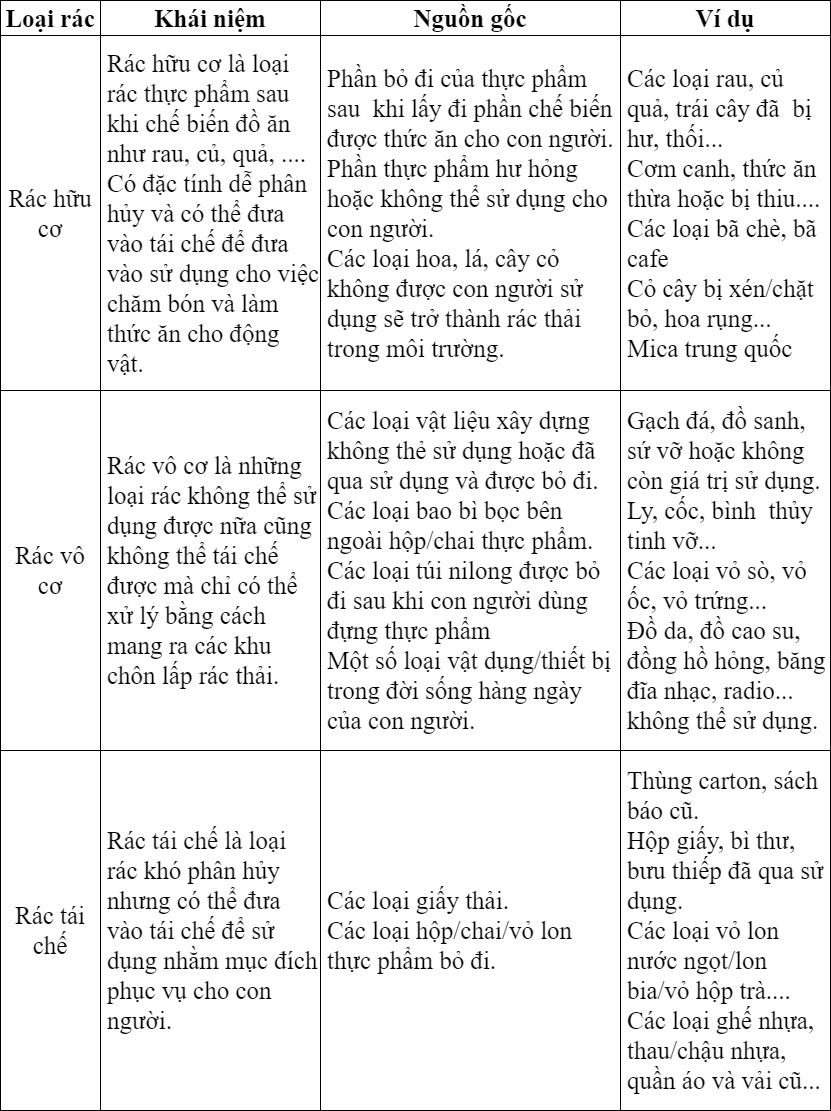
\includegraphics[width=\textwidth]{images/TraditionalTrash.png}
    \caption{Các loại rác truyền thống} 
    \label{tab.garbage.type}
\end{table}
Trong 3 loại chính, người ta còn định nghĩa cụ thể những loại rác khác:

% sửa cụ thể các loại rác thải thuộc loại nào.
\begin{itemize}
    \item Rác thải văn phòng: những văn phòng phẩm không còn được sử dụng (giấy báo cũ,  bút hết mực, …)
    \item Rác thải công nghiệp: loại rác có thành phần cực kỳ độc thải ra từ các nhà máy, công xưởng,… (chất ngâm tẩm, tẩy rửa, chất hóa học, phế liệu công nghiệp, thuốc trừ sâu bọ, thuốc kích thích tăng trưởng…) 
    \item Rác thải xây dựng: loại rác được thải ra môi trường từ những công trình xây dựng, sửa chữa, còn được gọi là xà bần (gạch, đá, vụn đất, …)
    \item Rác thải y tế: loại rác được thải ra từ các cơ sở y tế, bệnh viện, bệnh xá, được phân loại cụ thể như sau:
   \begin{itemize}
    \item Chất thải y tế lây nhiễm: gồm các chất thải lây nhiễm sắc nhọn (kim tiêm, lưỡi dao mỗ, đinh, cưa, kim chọc dò, …) và không sắc nhọn (chất thải thấm, dính máu hoặc dịch sinh học cơ thể, chất thải phát sinh từ buồng cách ly, …), chất thải có nguy cơ lây nhiễm cao (mẫu bệnh phẩm, dụng cụ đựng, dính mẫu bệnh phẩm phát sinh từ các phòng xét nghiệm an toàn sinh học …) và chất thải giải phẫu (mô, bộ phận cơ thể người thái bỏ và xác động vật thí nghiệm)
    \item Chất thải y tế nguy hại không lây nhiễm: gồm hóa chất, dược phẩm thải bỏ có các thành phân nguy hại, thiết bị y tế vỡ, hỏng, đã qua sử dụng có chứa thủy ngân hoặc kim loại nặng, chất hàn răng amalgam thải bỏ
    \item Chất thải y tế thông thường: gồm chất thải rắn trong sinh hoạt thường ngày của con người, chất thải ngoại cảnh trong cơ sở y tế và chất thải lỏng không nguy hại.
   \end{itemize}   
\end{itemize}

Vì thế, việc phân loại rác mang một vài ý nghĩa quan trọng đối với môi trường tự nhiên và cộng đồng xã hội:
\begin{itemize}
    \item Nhằm giảm thiểu tổng lượng rác thải từ cộng đồng ra môi trường do đó góp phần làm không khi trong lành và giảm thiểu nguy cơ ô nhiễm môi trường. 
    \item Giảm thiểu nguy cơ phát tán các tác nhân gây bệnh, các yếu tố độc hại, nguy hiểm. 
    \item Hạn chế nước rỉ rác góp phần làm giảm ô nhiễm nguồn đất, nguồn nước ngầm, nước mặt, giảm nhiều diện tích chôn lắp rác sinh hoạt. 
    \item Ngoài ra, phân loại rác còn có ảnh hưởng đến chất lượng cuộc sống của con người đem lại một lượng lớn các sản phẩm tái chế, mang lại hiệu quả kinh tế cho chính người thải rác bằng cách bán các nguyên, phế liệu có thể tái chế được, tận dụng các nguyên liệu hữu cơ sản xuất phân bón vi sinh.
    \item Góp phần nâng cao ý thức cuộc của cộng đồng về bảo vệ môi trường cũng như sử dụng tài nguyên hợp lý, nhất là ở trẻ nhỏ.
    \item Xây dựng một xã hội với môi trường xanh-sạch-đẹp.
    \item Nhằm giảm tải công tác xử lý, nhất là trong phương pháp đốt chất thải, đồng thời có thể lựa chọn phương pháp xử lý chất thải rắn phù hợp nhất.
    \item Giảm thiểu tổng lượng rác thải ra môi trường tiết kiệm chi phí thu gom, vận chuyển và xử lý.    
\end{itemize}

% Các cách phân loại rác truyền thống hiện nay là gì? (nói thêm về quy trình xử lí rác thải, từ việc thu gôm đến cách xử lí của nhà máy, chôn đốt rác plapaa => gây ảnh hưởng đến môi trường.)

Trước đây, quá trình phân loại rác thải sẽ do các cơ sở thu gom rác thực hiện nhưng vì tổng lượng rác thải từ nhiều nguồn được thải ra ngày càng nhiều nên việc huy động người dân phân loại rác tại nguồn là cách được sử dụng rộng rải nhất. Cách phân loại sẽ tùy thuộc vào mỗi địa phương quy định chi tiết, ở Việt Nam sẽ chia thành 3 danh mục: rác vô cơ, rác hữu cơ và rác tái chế. Các cơ sở thu gom rác sẽ tiến hành thu gom tận nơi và vận chuyển đến điểm tập trung, lượng rác được phân loại sẽ được xử lý theo 3 phương pháp sau:
\begin{itemize}
    \item Chế biến rác thải thành phân compost: chế biến rác hữu cơ dễ phân hủy thành phân compost dùng trong nông nghiệp, chia thành 2 quy mô chế biến:
        \begin{itemize}
            \item Quy mô chế biến tập trung: Rác hữu cơ dễ phân hủy được tách ly, nghiền, ủ hiếu khí để tạo ra phân vi sinh. Việc thành lập nhà máy chế biến phân compost cần vốn đầu tư lớn, chi phí vận hành cũng tương đối cao.
            \item  Quy mô chế biến hộ gia đình: Rác hữu cơ dễ phân hủy được ủ thành phân compost ngay trong sân vườn
        \end{itemize}

    \item Chôn lấp hợp vệ sinh: Rác thải được rải thành từng lớp dưới hố, đầm nén để giảm thể tích và phủ đất lên (phun  hóa chất để tăng hiệu quả xử lý nhanh và hạn chế côn trùng) với sơ đồ quy định như hình \ref{fig:so_do_chon_lap}:
    
        \begin{figure}[H]
            \centering            
            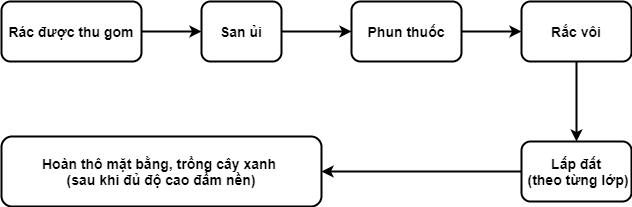
\includegraphics[width=\textwidth]{images/SoDoChonLap.png}
            \caption{Sơ đồ chôn lấp} \cite{trashclassification}
            \label{fig:so_do_chon_lap}
        \end{figure}

    \item Thiêu đốt: Rác thải được phân hủy ở nhiệt độ cao (1000 – 1100°C), giảm đáng kể thể tích chất thải phải chôn lấp (xỉ, tro), tuy nhiên chi phí đầu tư, vận hành nhà máy đốt rác khá cao, phù hợp với các nước tiên tiến, phát triển. 
   

\end{itemize}
Ngoài ra, một số khu vực khác sẽ có cách phân loại rác theo 4 loại lớn: 
    \begin{itemize}
        \item Rác dễ cháy (rác thải từ nhà bếp, giấy vụn, vải quần áo).
        \item Rác khó cháy (kim loại, thủy tinh, sành sứ).
        \item Rác tái chế (chai, bình, can, giấy báo).
        \item Rác cỡ lớn (đồ gia dụng cỡ lớn).
    \end{itemize}
  

Đồng nghĩa với việc rác thải được phân chia vào từng loại khác nhau, là tính chất của các loại rác cũng sẽ khác nhau. Như vậy, từng loại phải có cách xử lý riêng.

Mỗi địa phương sẽ quy định chi tiết cách phân loại rác khác nhau, nhưng cách truyền thống nhất nhất và được sử dụng rộng rãi nhất là chia rác thành 3 danh mục: rác vô cơ, rác hữu cơ và rác tái chế.
Ngoài ra, một số khu vực khác sẽ có cách phân loại rác theo 4 loại lớn: rác dễ cháy (rác thải từ nhà bếp, giấy vụn, vải quần áo), rác khó cháy (kim loại, thủy tinh, sành sứ), rác tái chế (chai, bình, can, giấy báo) và rác cỡ lớn (đồ gia dụng cỡ lớn)

\subsection{Phân loại sử dụng Internet of Things}
% Internet of things là gì 
Internet of Things (IoT) là một hệ sinh thái (được gọi là \qq{thiết bị kết nối} và \qq{thiết bị thông minh}), nhà cửa và các trang thiết bị khác được nhúng với các bộ phận điện tử, phần mềm, cảm biến, cơ cấu chấp hành cùng với khả năng kết nối mạng máy tính giúp cho các thiết bị này có thể thu thập và truyền tải dữ liệu
% Sự phổ biến của IoT 
Internet of Things đang dần trở nên quen thuộc và trở thành một trong số các trào lưu của nền công nghiệp hóa 4.0.
Không khó để có thể bắt gặp những sản phẩm thuộc lĩnh vực này, từ những sản phẩm gần gũi trong đời sống gia đình như đèn điều khiển bằng âm thanh, cửa thông minh...cho đến các sản phẩm giúp ích trong nông nghiệp như hệ thống tưới tiêu cho hoa màu từ xa, theo dõi các yếu tố về môi trường .... 
% Ưu điểm phân loại rác kết hợp IoT
Chưa dừng lại ở đó, khi xã hội càng phát triển, việc kết hợp các phần kiến thức độc lập với nhau thành một thể thống nhất để nâng cao chất lượng của sản phẩm tạo ra là điều hết sức cần thiết.
Điều đó được chứng minh rõ ràng qua việc bắt đầu có các sản phẩm IoT sử dụng kỹ thuật Machine Learning được ra đời và ứng dụng vào các lĩnh vực, vấn đề mà xã hội đang quan tâm.
Trong đó, bằng cách tạo ra các sản phẩm sử dụng công nghệ tiên tiến nói trên vào mục đích bảo vệ môi trường đang là một trong các ý tưởng thiết thực, đáp ứng nhu cầu của xã hội.
 
%Sửa so sánh với cái chung 
Ở các nước khác, việc cung cấp các loại thùng rác với từng loại rác đã trở nên phổ biến, và yêu cầu mọi người phải tự giác thực hiện việc bỏ rác đúng quy định, đúng thùng rác. Một số ví dụ cụ thể như:
Ở Nhật, việc bỏ rác được quy định ngay trên các tấm lịch, người dân cần phân loại rác và bỏ rác đúng loại rác vào ngày được quy định trên lịch nếu trường hợp ở hộ gia đình. Và các thùng rác công cộng cũng được kí hiệu phân loại rác, người dân phải bỏ đúng loại rác vào thùng rác có kí hiệu phân loại. Hoặc ở một số nước khác, như Singapore đã áp dụng các quy định cứng rắn đối với người dân và cả khách du lịch nếu họ vứt rác bừa bãi, mức phạt có thể lên đến 1,000 SGD (17 triệu đồng). Tuy nhiên, ở Việt Nam lại khá khó áp dụng như thế, về khách quan mà nói thì ta dễ dàng nhận thấy hệ thống thùng rác công cộng được bố trí trên đường khá thưa thớt, nên người dân khó tìm được nơi bỏ rác khi tham gia giao thông, và một mặt hạn chế mà chúng ta cần nhìn nhận là có một bộ phận không nhỏ người dân có ý thức chưa tốt, chưa thực hiện bỏ rác đúng nơi quy định cũng như chưa hình thành thói quen phân loại rác. Đa số  chúng ta đều để chung tất cả các loại rác thải vào một bao sau đó để nhân viên dọn vệ sinh gôm về nhà máy xử lý. Quy trình và các ảnh hưởng xấu của việc xử lí rác thải truyền thống như đã nêu ở mục trên, vì thế việc thiết kế thùng rác kết hợp IoT tự động phân loại rác và hệ thống quản lý vị trí thùng rác cũng như lượng rác trong mỗi thùng được cập nhật liên tục mỗi giờ sẽ mang lại rất nhiều lợi ích: Giảm bớt quy trình xử lý, giảm công sức lao động, giảm tiền của, và mang tính quản lý chủ động cao.



\section{Previous work}
% Đã có những đề tài, bài báo nào liên quan đến việc dùng IoT trong phân loại rác, tóm tắt nội dung từng bài. 4-5 bài là xong mục này,

% so sánh các ưu nhược điểm của các đề tài, họ làm được tới đâu.  
Trong công bố  \cite{trashnet}, hai tác giả đã cho rằng:

Dùng thị giác máy tính để phân loại tái chế rác sẽ mang lại nhiều hiệu quả đối với việc xử lý rác thải. Đối tưọng của bài toán này là dùng hình ảnh của một loại rác tái chế hoặc rác thải thông thường và phân loại chúng vào 6 lớp: thủy tinh, giấy, kim loại, nhựa, bìa cứng, và rác thải khác. Mindy Yang và Gary Thung cũng tạo ra một dataset bao gồm mỗi lớp khoảng 400 - 500 hình ảnh được thu thập một cách thủ công. Họ dự kiến công khai tập dataset cho cộng đồng. Hai model được sử dụng là: SVM (Support Vector Machine) với SIFT (Scale-Invariant Feature Transform) và CNN (Convolutional Neural Network). Các thử nghiệm của họ chỉ ra rằng SVM có hiệu quả cao hơn CNN. Tuy nhiên, CNN chưa được huấn luyện một cách tốt nhất do gặp nhiều khó khăn trong việc xác định siêu tham số.

Trong công bố  \cite{smartcity}, hai tác giả đã cho rằng:

Hiện nay, những khu đô thị, thành phố lớn đang dần được chuyển hóa để trở nên \qq{thông minh} hơn. Bên cạnh một số hệ thống quản lý thông minh phổ biến (giao thông, đèn, năng lượng, ...) thì hệ thống xử lý rác thải thông minh là một phần không thể thiếu cho bất kỳ một thành phố thông minh nào. 
Một hệ thống rác thải thông minh nhắm vào việc giải quyết lượng rác trong những khu công cộng hoặc ngoại ô. Ngoài việc mất mỹ quan đô thị của một khu vực, rác thải có thể gây ô nhiễm và ảnh hưởng trầm trọng đến chất lượng cuộc sống của người dân trong khu vực đó. Luận văn tập trung vào việc phát triển phần mềm có thể nhận diện lượng rác thải thông qua việc phân tích các luồng video ở thời gian thật. Mô hình mạng cải tiến YOLOv3 được triển khai để thực hiện chức năng phát hiện rác. Hệ thống đã được điều chỉnh thích hợp theo dataset đã được sưu tầm cho mục đích này.  

Kết quả cho thấy cách tiếp cận như trên đã đóng góp một phần to lớn vào việc quản lý rác thải hiệu quả hơn ở những thành phố thông minh.

Trong công bố \cite{lstmprediction1}, tác giả cho rằng dự báo chuỗi thời gian là một vấn đề quan trọng trong nhiều lĩnh vực, một dự đoán tốt chính là bằng chứng cốt yếu để mọi người đưa ra quyết định.

Đối với những mô hình thực hiện phương pháp dựa trên kiến thức thông kê, chúng hoạt động rất tốt với việc dự đoán một bước tiếp theo, nhưng khi tiến hành dự đoán nhiều bước tiếp, hiệu suất của một vài mô hình không đạt được như mong đợi. Vì thế, tác giả đã gợi ý sử dụng mô hình mạng LSTM (Long-Short Term Memory) để giải quyết bài toán mà không cần bận tâm đến nhiều bước thủ công trong các phương pháp mô hình hóa truyền thống, chẳng hạn như kiểm tra độ ổn định, hàm tự tương quan, hàm tự tương quan từng phần,...

Khi xét về chuỗi thời gian, có rất nhiều dữ liệu trong cuộc sống hằng ngày của chúng ta có thể được mô hình hóa thành chuỗi thời gian, như chỗ đậu xe còn lại trong bải đậu xe thay đổi theo giờ, số lượng khách đến bảo tàng mỗi ngày, chi phí điện cho trung tâm mua sắm hằng tháng,... Các chuỗi thời gian khác nhau có các đặc điểm khác nhau, một số có thể có giá trị trung bình xung quanh 0, một số có tính chất tuần hoàn, một số có tính chất tăng/giảm, cho nên xây dựng một mô hình phù hợp với nhiều loại chuỗi dữ liệu khác nhau là một nhiệm vụ khó khăn.

Kết quả bài báo cho thấy mô hình LSTM khá phù hợp với phạm vi rộng lớn các mẫu dữ liệu, nhưng các mẫu dữ liệu trong bài báo tương đối đơn giản và vẫn còn rất nhiều không gian khai thác trong lĩnh vực dữ đoán chuỗi thời gian đi trước nhiều bước.

\section{Mục tiêu nghiên cứu}
% Trên cơ sở vấn đề đã đặt, khóa luận dự kiến làm gì
%  Xây dựng thùng rác thông minh phân loại rác dựa trên hình. Mô tả kết cấu thùng, phân mấy loại rác, v.v...
%  Các chức năng xử về dữ liệu1
Nắm bắt xu thế trên, bài toán được đặt ra là phải tạo ra sản phẩm vừa đáp ứng được yêu dễ triển khai trên diện rộng, nhằm giảm sức người, tiết kiệm, mà người quản lý dễ kiểm soát, dễ sử dụng, sửa chữa.
Từ đó, đề tài về \qq{Xây dựng mô hình thùng rác thông minh dựa trên công nghệ trí tuệ nhân tạo} đã được ra đời để giải quyết bài toán đó. 
Thùng rác tự động phân loại rác áp dụng kỹ thuật Machine Learning để giảm thiểu thời gian, sức người cũng như các dây chuyển xử lí phân loại rác như trước đây, từ đó tiết kiệm được các khoản chi phí.
Tuy nhiên, việc thực hiện hóa đề tài trên đã gặp không ít nhũng khó khăn, để giảm thiểu chi phí thiết kế, cũng như hướng đến việc khả thi khi đưa vào thực tế.

Nhóm đưa ra phương hướng thiết kế phải đảm bảo các tiêu chí: giá thành hợp lí, tiết kiệm điện năng, và có thể sử dụng ở nhiều môi trường (đặc biệt là các khu vực khó cung cấp nguồn điện).
Để thực hiện các phương hướng đã đưa ra, nhóm chọn sử dụng mạch ESP32 CAM với giá thành cạnh tranh hơn rất nhiều so với sản phẩm dùng raspberry pi.
Ngoài ra, hướng đến nguồn năng lượng tiết kiệm và thân thiện hơn với môi trường, nhóm sử dụng pin năng lượng mặt trời để nạp vào nguồn pin dự trữ.
Như vậy, thùng rác vẫn có thể hoạt động được vào cả ban ngày lẫn ban đêm, và có khả năng nạp nguồn từ việc chuyển hóa từ quang năng sang điện năng để cung cấp cho thùng rác hoạt động.

Khác với bộ xử lý mạnh mẻ có thể lên đến 16GB của raspberry pi cùng với các công cụ hỗ trợ phong phú, thì ESP32 CAM chỉ có bộ xử lý vỏn vẹn 4MB.
Cũng vì sự khác biệt đó cộng thêm việc sử dụng Machine Learning vào các thiết bị nhúng vẫn là một xu thế khá mới mẻ, dẫn đến việc nhóm đã gặp rất nhiều khó khăn và thách thức khi thực hiện đề tài này.
Đối với các microcontroller như ESP32, việc có thể thực hiện các tác vụ như chụp hình và trả kết quả phân loại rác đã phải mất nhiều thời gian.
Thách thức lớn nhất là phải đưa được model đã train vào mạch có bộ nhớ thấp nhưng vẫn đảm bảo độ chính xác ở mức có thể chấp nhận. 

Để giải quyết thách thức đó, nhóm em đã sử dụng Google Colab để train model sau đó sử dụng TensorFlow Lite để có thể đưa model đã train vào thiết bị nhúng bằng môi trường Espress IF.
Với thiết kế tối giản, thùng rác sẽ vận hành theo các bước như sau: 
\begin{itemize}
    \item Bước 1: Thiết bị sẽ chụp hình vật thể sau khi vật thể đó được để vảo khay đụng rác
    \item Bước 2: Hình ảnh sẽ được chuyển sang một chuỗi byte sau đó áp dụng model đã train để đưa ra kết quả phân loại. Nếu là nhựa, thủy tinh thì sẽ đem tái chế, còn nếu là giấy, và các loại rác khác thì sẽ không tái chế.
    \item Bước 3: Rác sẽ rơi vào một trong hai khay đựng rác bên trong theo đúng kết quả đã đưa ra.
\end{itemize}
Như vậy, việc phân loại đã trải qua ba bước như trên.
Có thể thấy rằng, so với việc sử dụng raspberry pi, các microcontroller như ESP32 CAM đã giải quyết bài toán một cách nhanh chóng hơn bằng cách tự thực hiện quá trình xử lý ảnh và phân loại thay vì đưa hình lên server để xử lý sau đó trả kết quả ngược về cho raspberry pi.
Ngoài ra, nhóm còn sử dụng công nghệ LoRaWan để truyền dữ liệu về mực rác còn lại trong thùng.

Bên cạnh đó, chúng tôi cần phải xây dựng một hệ thống để quản lý tất cả thông tin thùng rác và xử lý dữ liệu realtime thu được từ cảm biến và một giao diện để hiển thị tất cả thông tin đó. Mô hình bao gồm: 1 Nodejs làm server trung tâm nhận và xử lý các dữ liệu từ thiết bị gửi tới và mô phỏng các thiết bị ảo khác, 1 Python server để tiên đoán lượng rác sau nhiều bước thời gian thông qua Deep Learning và sử dụng giao diện của Thingsboard để hiển thị thông tin và dữ liệu thiết bị.

Ngoài ra, chúng tôi còn sử dụng 1 open-source server Thingsboard cung cấp các API liên quan đến việc quản lý thiết bị, cảm biến (bao gồm tạo, sửa, xóa, …) và hiển thị, lưu trữ dữ liệu trên Dashboard, 1 open-source server từ Mapbox cung cấp các API liên quan đến xử lý tọa độ địa lý và cung cấp đường đi tối ưu cho đến các thiết bị.

Server chính sẽ nhận dữ liệu từ cả thiết bị thật và ảo để xử lý và gửi lên Thingsboard để hiển thị, dữ liệu từ thiết bị thật sẽ được gửi từ gateway The Things Network (TTN) với một format nhất định, vì thế thiết bị ảo cũng sẽ được lập trình để gửi dựa theo format đó. Thiết bị thật và ảo đều có những chức năng giống nhau (tạo, liên kết, gửi dữ liệu, …), nhưng cách xử lý thì khác nhau, cụ thể theo bảng \ref{tab.function}

\begin{table}[H]
    \caption{Chức năng} 
    \label{tab.function}
    \centering
    \begin{tabular}{|l|l|l|}
        \hline
        Chức năng    & Thiết bị thật                                                                                            & Thiết bị ảo                                                                                                                                                            \\ \hline
        Tạo thiết bị & \multicolumn{2}{l|}{\begin{tabular}[c]{@{}l@{}}Được tạo thủ công trực tiếp trên Thingsboard hoặc gửi \\ request body đến API của Server để tạo tự động\end{tabular}}                                                                                                              \\ \hline
        Tạo cảm biến & \multicolumn{2}{l|}{\begin{tabular}[c]{@{}l@{}}Các cảm biến cũng được tạo tự động sau khi thiết bị được tạo \\ và được liên kết mỗi quan hệ tự động với thiết bị\end{tabular}}                                                                                                    \\ \hline
        Gửi dữ liệu  & \begin{tabular}[c]{@{}l@{}}Dữ liệu được gửi thông \\ qua gateway TTN theo \\ format cố định\end{tabular} & \begin{tabular}[c]{@{}l@{}}Dữ liệu được random từ file .csv, \\ tính toán lại và được định dạng \\ theo format của thiết bị thật và \\ được gửi về server\end{tabular} \\ \hline
    \end{tabular}
\end{table}

Sau khi dữ liệu được gửi về server thì các chức năng sẽ được xử lý chung:
\begin{itemize}
    \item Dữ liệu được gửi về sẽ được gửi lên Thingsboard để hiển thị, đồng thời được lưu trữ vào file csv của từng thiết bị.
    \item Các file csv sẽ được gửi qua Python server để tiên đoán lượng rác sau mỗi khoảng thời gian trước khi quá trình thu gom rác bắt đầu, kết quả sẽ trả về Node server và được xử lý tiếp.
\end{itemize}





% !TEX root = ..\thesis.tex

\chapter{CƠ SỞ LÍ THUYẾT}

% các cách sử dụng để giải quyết bài toán
\section{Bài toán phân loại ảnh và kỹ thuật học sâu (Deep learning)}
Phân loại ảnh là một bài toán phổ biến trong lĩnh vực thị giác maý tính. Mục tiêu của bài toán là làm cho máy tính có khả năng xác định nhãn của hình ảnh. Cụ thể hơn bài toán có đầu vào và đầu ra như sau:

- Đầu vào: Ảnh chứa đối tượng cần xác định nhãn và danh sách các nhãn (labels).

- Đầu ra: nhãn tương ứng với đối tượng trong ảnh đầu vào.

% kiếm đại hình phân loại ảnh nào cũng được, có liên quan đến đề tài càng tốt
Hình minh họa đầu vào và đầu ra của bài toán. Bài toán này được áp dụng trong nhiều lĩnh vực như: phân loại biển báo giao thông, phân loại chữ viết tay,... Các phương pháp giải quyết bài toán được chia làm hai loại: tiếp cận dựa trên máy học và học sâu. Đối với cách tiếp cận dựa trên máy học trước tiên cần phải xác định các đặc trưng từ hình ảnh bằng một số phương pháp như: Scale-invariant feature transform (SIFT), Histogram of oriented gradients (HOG). Sau đó sử dụng thêm một số kỹ thuật phân lớp như thuật toán Support vector machine (SVM) hoặc Decision Tree để phân loại đối tượng. 

Cách tiếp cận dựa trên học sâu sử dụng kiến trúc mạng Convolution neural network cho cả việc trích xuất đặc trưng và phân loại đối tượng. Ngoài ra ta có thể kết hợp cả hai phương pháp bằng cách sử dụng mạng Convolution neural network để trích xuất đặc trưng sau đó sử dụng các kỹ thuật phân lớp để phân loại đối tượng. 

Trong những năm gần đây, sự phát triển của khoa học kỹ thuật và lượng dữ liệu ngày càng lớn đã tạo điều kiện cho các kiến trúc mạng CNN được áp dụng ngày càng nhiều trong việc giải quyết các bài toán phân loại ảnh. Các mô hình này cũng mang lại kết quả cao với thời gian ngắn đủ để đáp ứng yêu cầu áp dụng trong các bài toán real-time của con người. Chính vì vậy chúng tôi đã sử dụng thuật toán CNN cho khóa luận này.

\section{Kiến trúc mạng học sâu CNN}
CNN là một kiến trúc mạng bao gồm các lớp: convolution layer + nonlinear layer, pooling layer, fully connected layer liên kết với nhau theo một thứ tự nhất định. Thông thường, ảnh được truyền qua lớp convolution + nonlinear sau đó đến pooling layer. Bộ ba convolution + nonlinear và pooling layer được lặp lại nhiều lần trong mạng. Sau đó các giá trị tính toán được lan truyền qua tầng fully connected và softmax để phân loại đối tượng trong ảnh. Hình minh họa mạng CNN cơ bản.

Trong kiến trúc mạng này ảnh đầu vào được biểu diễn dưới dạng ma trận. Lớp Convolution được sử dụng để phát hiện đặc trưng cụ thể của ảnh, từ các đặc trưng cơ bản như góc, cạnh đến các đặc trưng phức tạp như texture của ảnh. Một ma trận có kích thước nhỏ (3x3 hoặc 5x5) được gọi là filter sẽ lướt qua toàn bộ ảnh từ trái sang phải và từ trên xuống dưới để phát hiện các đặc trưng trong ảnh. 

\begin{figure}

    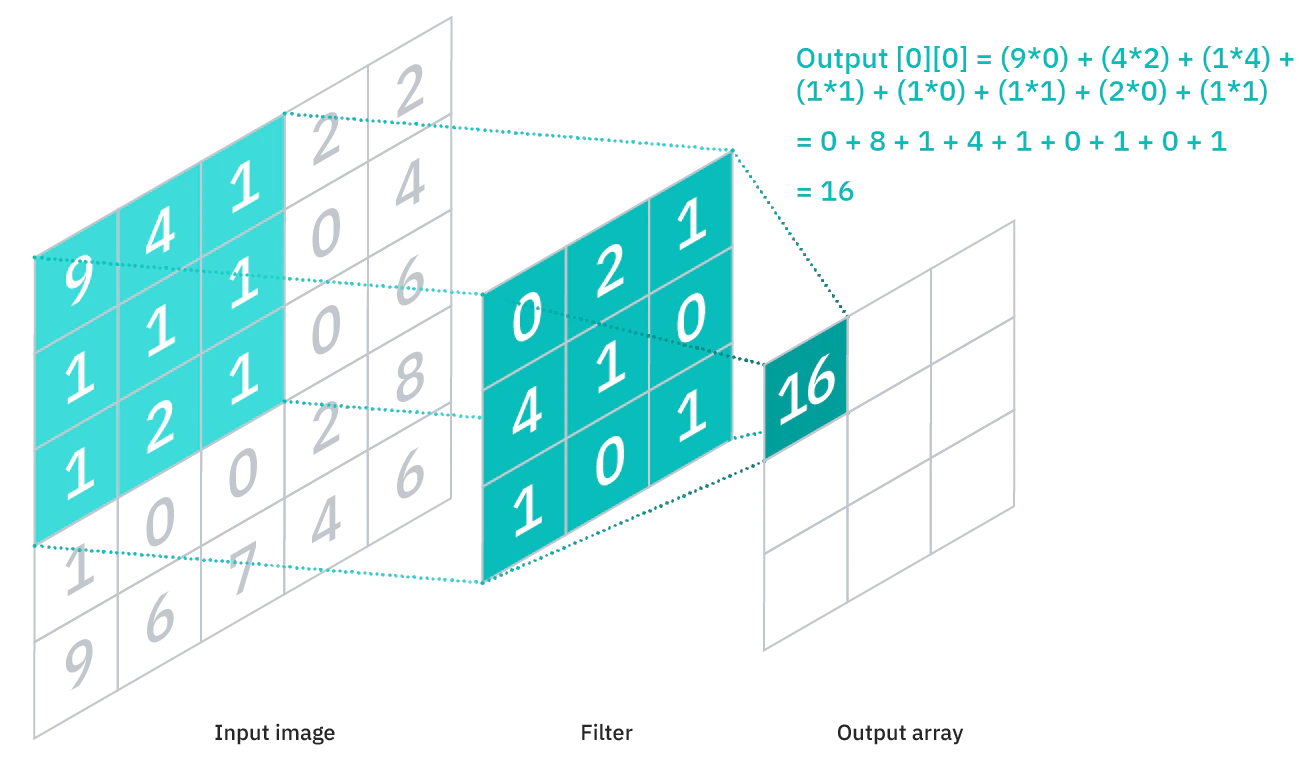
\includegraphics[width=\textwidth]{images/Quanh/cnn.png}
    \caption{Ví dụ về phép tính convoluted cho neural network}
\end{figure}

Kích thước của filter tỉ lệ thuận với số tham số cần học và thường là số lẻ. Sau khi áp dụng phép convolution thì ma trận đầu vào sẽ nhỏ dần dẫn đến số layer của mô hình CNN bị giới hạn. Vì vậy cần phải lưu ý đến tham số stride, thể hiện số pixel cần phải dịch chuyển mỗi khi trượt filter trên ảnh và thêm padding có giá trị bằng 0 ở phần khung của ảnh. Tương tự như mạng neurald network, CNN cũng sử dụng hàm kích hoạt như ReLU hoặc tanh đặt ngay sau tầng convolution. Đối với dữ liệu ảnh hàm kích hoạt thường được sử dụng là ReLU, hàm này gán những giá trị âm bằng 0 và giữ nguyên các giá trị lớn hơn 0.

Pooling layer được xếp sau các lớp convolution để giảm tham số. Các loại pooling được sử dụng chủ yếu là max pooling và average. Các lớp này sẽ được lặp lại theo thứ tự để tạo ra feature map cuối cùng sau đó truyền vào tầng fully connected. Tầng này chuyển ma trận nhận được thành vector và phân loại vector đó tương tự như mạng neural network.

% dùng CNN giải quyết bài toán gì, lý thuyết về CNN, còn các phần khác của QUyết đưa vào mục dưới ( mục đóng góp)
% Mạng CNN là một tập hợp các lớp Convolution chồng lên nhau và sử dụng các hàm nonlinear activation như ReLU và tanh để kích hoạt các trọng số trong các node. CNN được dùng trong trong nhiều bài toán như nhân dạng ảnh, phân tích video, ảnh MRI, hoặc cho bài các bài của lĩnh vự xử lý ngôn ngữ tự nhiên. Trong đề tài này, chúng tôi đã sử dụng mạng CNN để giải quyết bài toán phân loại rác.
% Bài toán có đầu vào là một hình ảnh của rác được đưa vào thùng và đầu ra là nhãn của loại rác đó.
% CNN bao gồm tập hợp các lớp cơ bản bao gồm: convolution layer + nonlinear layer, pooling layer, fully connected layer. 
% Các lớp này liên kết với nhau theo một thứ tự nhất định. 
% Thông thường, một ảnh sẽ được lan truyền qua tầng convolution layer + nonlinear layer đầu tiên, sau đó các giá trị tính toán được sẽ lan truyền qua pooling layer, bộ ba convolution layer + nonlinear layer + pooling layer có thể được lặp lại nhiều lần trong network. Và sau đó được lan truyền qua tầng fully connected layer và softmax để tính xác suất ảnh đó chứa vật thế gì.

\label{chap:ontology}
\section{Giới thiệu TensorFlow và TensorFlow Lite}
%TensorFlow Lite is an open source deep learning framework for on-device inference.
TensorFlow Lite là giải pháp gọn nhẹ của TensorFlow cho thiết bị di động và thiết bị nhúng.
Nó cho phép suy luận học máy trên thiết bị với độ trễ thấp và kích thước nhị phân nhỏ.




\section{Giới thiệu công nghệ LoRaWan}
LoRa(long-range) sử dụng kỹ thuật điều chế gọi là Chirp Spread Spectrum.
Có thể hiểu nôm na nguyên lý này là dữ liệu sẽ được băm bằng các xung cao tần để tạo ra tín hiệu có dãy tần số cao hơn tần số của dữ liệu gốc (cái này gọi là chipped); sau đó tín hiệu cao tần này tiếp tục được mã hoá theo các chuỗi chirp signal (là các tín hiệu hình sin có tần số thay đổi theo thời gian; 
Có 2 loại chirp signal là up-chirp có tần số tăng theo thời gian và down-chirp có tần số giảm theo thời gian; và việc mã hoá theo nguyên tắc bit 1 sẽ sử dụng up-chirp, và bit 0 sẽ sử dụng down-chirp) trước khi truyền ra anten để gửi đi.

Theo Semtech công bố thì nguyên lý này giúp giảm độ phức tạp và độ chính xác cần thiết của mạch nhận để có thể giải mã và điều chế lại dữ liệu; hơn nữa LoRa không cần công suất phát lớn mà vẫn có thể truyền xa vì tín hiệu Lora có thể được nhận ở khoảng cách xa ngay cả độ mạnh tín hiệu thấp hơn cả nhiễu môi trường xung quanh.
Băng tần làm việc của LoRa từ 430MHz đến 915MHz cho từng khu vực khác nhau trên thế giới:

430MHz cho châu Á

780MHz cho Trung Quốc

433MHz hoặc 866MHz cho châu Âu

915MHz cho USA

LoRaWAN là giao thức mạng năng lượng thấp, diện rộng (LPWA) được phát triển bởi Liên minh LoRa, kết nối không dây ‘hoạt động’ với internet trong các mạng khu vực, quốc gia hoặc toàn cầu, nhắm mục tiêu các yêu cầu chính của Internet of Things (IoT) như bi thông tin liên lạc hai chiều, dịch vụ bảo mật đầu cuối, di động và nội địa hóa.
LoRaWAN sử dụng phổ không được cấp phép trong các dải ISM để xác định giao thức truyền thông và kiến ​​trúc hệ thống cho mạng trong khi lớp vật lý LoRa tạo ra các liên kết giao tiếp tầm xa giữa các cảm biến từ xa và các cổng kết nối với mạng. Giao thức này giúp thiết lập nhanh chóng các mạng IoT công cộng hoặc riêng tư ở bất cứ đâu bằng phần cứng và phần mềm.

\section{LoRa và LoRaWAN khác nhau như thể nào}

\begin{figure}[H]
    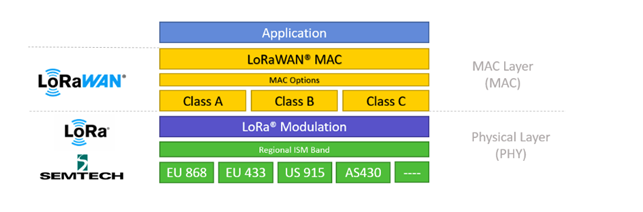
\includegraphics[width=\textwidth]{images/Quanh/LoraWan_Stack.png}
    \caption{LoRaWAN Technology Stack}
    \label{fig:lorawan_stack}
\end{figure}

Cả hai thuật ngữ thường được sử dụng đồng nghĩa, nhưng chúng có ý nghĩa khác nhau. Nhìn vào hình \ref{fig:lorawan_stack}, ta có thể thấy:
\begin{itemize}
    \item LoRa là chip (Physical layer) để giao tiếp không dây giữa Gateway và node thông qua tần số
    \item LoRaWan nằm ở MAC layer là giao thức mạng bao gồm việc sử dụng chip LoRa để liên lạc
\end{itemize}

\section{The Things Networks}
Là hệ thống bao gồm các vai trò Network Server, Application Server, join server

\subsection{Network Server}
Tư hình \ref{fig:lorawan_network}, ta suy được:
\begin{figure}[h]
    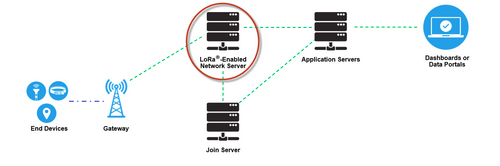
\includegraphics[width=\textwidth]{images/Quanh/LoraWan_Netwrok.png}
    \caption{Mô hình LoRaWAN Network}
    \label{fig:lorawan_network}
\end{figure}

\begin{itemize}
    \item Nhận data từ sensor của các end-devices thông qua Gateway
    \item Thực tế, các Network sẽ:
    \begin{itemize}
        \item Kiểm tra device address
        \item Đếm và quản lí số frame thực tế
    \end{itemize}
\end{itemize}

\subsection{Application Server}
Quản lí và hiển thị data, thực hiện các thao tác tạo ra down-link payload để kết nối đến end- device

\subsection{Join Network}
Trên the things network, có 2 hình thức join: OTAA ( over-the-air activation) và ABP( Activation by Personalization) có đặc điểm như bảng \ref{tab.network.otaa}

\begin{table}[H]
    \centering
    \caption{So sánh giữa OTAA và ABP} 
    \label{tab.network.otaa}
    \begin{tabular}{| m{6cm} | m{6cm} |}
        \hline
        OTAA & ABP \\

        \hline
        -	Bảo mật hơn & - Ít bảo mật \\
        -	Tự chọn channel join vào & - Setup channel ở end-device \\
        
        \hline
    \end{tabular}
\end{table}

\section{LoRa Dragino LG02 dual channel gateway}
Thiết bị được mô tả ở hình \ref{fig:lora_gateway} với những đặc tính sau:
\begin{figure}[H]
    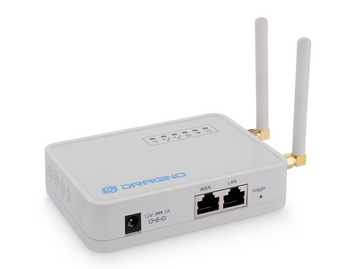
\includegraphics[width=\textwidth]{images/Quanh/lora_gateway.png}
    \caption{LG02 Dragino Gateway}
    \label{fig:lorawan_gateway}
\end{figure}

\begin{itemize}
    \item LG02 là open source dual channels LoRa Gateway. Là cầu nối dễ dàng cho LoRa wireless network và IP network: wifi, Ethernet, 3g/4g\dots .
    \item Hỗ trợ giải quyết từ 50-300 sensor nodes
    \item Frequency 433Mhz
\end{itemize}

\section{End-Device}
Kit RF thu phát wifi Blue esp32 + lora sx1278 oled heltec được mô tả như hình \ref{fig:lorawan_kit} với những đặc điểm sau:
\begin{figure}[H]
    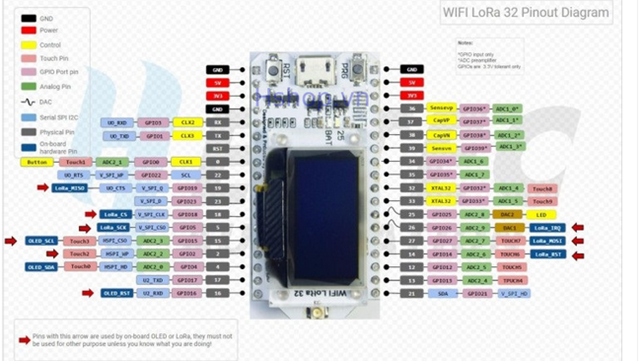
\includegraphics[width=\textwidth]{images/Quanh/lora_kit.png}
    \caption{Kit RF thu phát wifi Blue esp32 + lora sx1278 oled heltec}
    \label{fig:lorawan_kit}
\end{figure}
\begin{itemize}
    \item Ba chuẩn giao tiếp: wifi, BLE, RF Lora
    \item Frequency 433Mhz
\end{itemize}

\section{Sử dụng Nodejs và Python Server}
Nodejs là nền tảng được xây dựng trên V8 Javascript Engine, được thiết kế để xây dựng các ứng dụng lớn nhỏ và có thể mở rộng nhanh với chi phí ít tốn kém nhất.

Nodejs hoạt động trên một luồng duy nhất sử dụng I/O bất đồng bộ theo hướng sự kiện để duy trì trọng lượng nhẹ và hiệu quả khi đối mặt với các ứng dụng sử dụng nhiều dữ liệu chạy trên các thiết bị phân tán. Vì thế, nó tỏa sáng trong các ứng dụng mạng thời gian thực nhanh, và vì có khả năng xử lý một số lượng lớn các kết nối đồng thời với thông lượng cao, nó cho phép hàng chục nghìn kết nối đồng thời giữa máy khách và máy chủ được trao đổi dữ liệu tự do qua tương đương với khả năng mở rộng cao.

Python là ngôn ngữ lập trình hướng đối tượng đa dạng, sở hữu cấu trúc dữ liệu cấp cao và hệ thống thư viện lớn, được sử dụng linh hoạt vào nhiều mục đích như lập trình ứng dụng web, khoa học và phân tích dữ liệu, tạo nguyên mẫu phần mềm, ...

Việc sử dụng để tính toán nặng đòi hỏi nhiều tài nguyên CPU như Machine Learning hoặc Big Data không phải thế mạnh của Nodejs. Nên sử dụng Python sẽ phù hợp nhất với các dự án dựa trên AI và máy học vì tính đơn giản, linh hoạt và nhất quán, cũng như quyền truy cập vào nhiều thư viện và frameworks phong phú liên quan đến máy học, phân tích dữ liệu và tính toán khoa học, trực quan dữ liệu, ....

\section{Giới thiệu về LSTM và bài toán dự đoán chuỗi dữ liệu đa bước thời gian}
LSTM (Long Short-Term Memory) là phiên bản mở rộng của mạng RNN (Recurrent Neural Network), được thiết kế để giải quyết các bài toán về phụ thuộc dài hạn (long-term dependencies) trong mạng RNN do bị ảnh hưởng bởi vấn đề gradient biến mất.

Mạng LSTM có thể bao gồm nhiều LSTM memory cell liên kết với nhau và kiến trúc cụ thể của mỗi tế bào được biểu diễn như hình \ref{tab.lstm_cell}. Ý tưởng của mạng LSTM là bổ sung thêm trạng thái bên trong tế bào (cell internal state) $s_t$ và ba cổng sàng lọc các thông tin đầu vào và đầu ra cho tế bào bao gồm forget state $f_t$ (loại bỏ thông tin nhận được không cần thiết ra khỏi cell), input gate $i_t$ (chọn lọc thông tin cần thiết thêm vào cell) và output gate $o_t$ (xác định thông tin nào từ cell được sử dụng như đầu ra). Tại mỗi bước thời gian t, các cổng đều lần lượt nhận giá trị đầu vào $x_t$ (đại diện cho một phần tử trong chuỗi đầu vào), sau đó dựa trên cơ chế hoạt động của cell, đưa qua quá trình lan truyền xuôi (forward pass) và giá trị $h_{t-1}$ có được từ đầu ra của memory cell từ bước thời gian trước đó t - 1.

\begin{figure}[h]
    \caption{Sở đồ biểu diễn kiến trúc bên trong tế bào LSTM}
    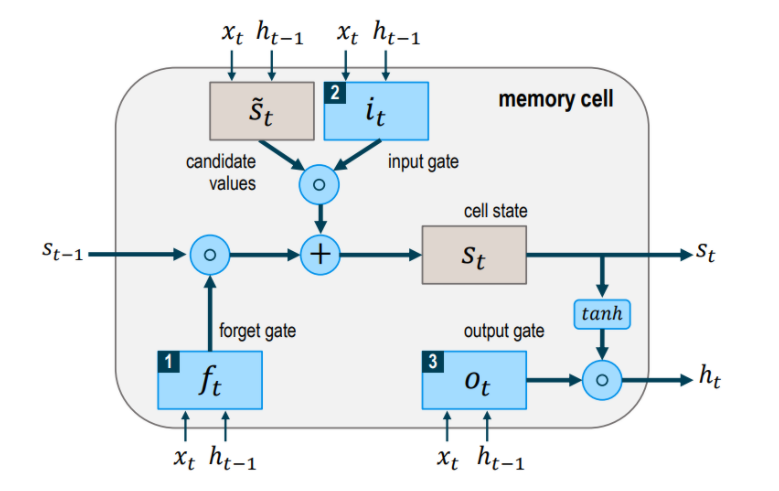
\includegraphics[width=\textwidth]{images/Khanh/Python/LSTM_cell_structure.PNG}
    \label{tab.lstm_cell}
\end{figure}

Dự đoán trước nhiều bước thời gian là công việc dự đoán một chuỗi các giá trị trong một chuỗi thời gian bằng việc áp dụng mô hình dự đoán từng bước và sử dụng giá trị dự đoán của bước thời gian hiện tại để xác định giá trị của nó trong bước thời gian tiếp theo. Hiện nay có ít nhất bốn chiến lược thường được sử dụng để giải quyết bài toán này:
\begin{itemize}
    \item Dự báo trực tiếp:
    \begin{itemize}
        \item Liên quan đến việc phát triển mô hình riêng biệt cho từng bước thời gian.
        \item Không thích hợp trong việc tính toán và bảo trì vì số lượng bước thời gian dự đoán đôi khi sẽ lên rất nhiều.
        \item Không có cơ hội để mô hình hóa sự phụ thuộc giữa các dự đoán.
    \end{itemize}
    \item Dự báo đệ quy:
    \begin{itemize}
        \item Liên quan đến việc sử dụng mô hình một bước nhiều lần trong đó dự đoán cho bước thời gian trước được sử dụng làm đầu vào để đưa ra dự đoán cho bước thời gian sau.
        \item Cho phép tích lũy các lỗi dự đoán để hiệu suất có thể nhanh chóng suy giảm khi thời gian dự đoán tăng lên.
    \end{itemize}
    \item Dự báo kết hợp:
    \begin{itemize}
        \item Kết hợp giữa trực tiếp và đệ quy để cung cấp các lợi ích của cả hai phương pháp và khắc phụ hạn chế của mỗi chiến lược.
        \item Phát triển mô hình cho từng bước thời gian dự đoán, nhưng mỗi mô hình có thể sử dụng các bước dự đoán được thực hiện bởi các mô hình ở các bước thời gian trước đó làm giá trị đầu vào.
    \end{itemize}
    \item Dự báo nhiều đầu ra:
    \begin{itemize}
        \item Liên quan đến việc phát triển một mô hình có khả năng dự đoán toàn bộ chuỗi dự báo theo cách một lần.
        \item Phức tạp hơn vì chúng có thể tìm hiểu cấu trúc phụ thuộc giữa đàu vào và đầu ra cũng như giữa các đầu ra.
        \item Mô hình đào tạo sẽ chậm hơn và yêu cầu nhiều dữ liệu hơn để tránh Overfitting cho vấn đề.
    \end{itemize}
\end{itemize}

\section{Giới thiệu bài toán TSP (Travelling Salesman Problem)}
TSP (bài toán người du lịch) là một bài toán tối ưu tổ hợp thuộc lớp phức tạp NP-hard, trình bày vấn đề: "Cho sẵn danh sách các thành phố và khoảng cách giữa những thành phố đó, tìm đường đi khả thi ngắn nhất từ điểm bắt đầu đến các thành phố và quay lại điểm bắt đầu, với điều kiện mỗi thành phố chỉ được đi qua một lần". 

Hiện tại đã có nhiều phương pháp giải quyết bài toán này thông qua các thuật toán chính xác, heuristic:
\begin{itemize}
    \item The Brute-Force Approach: Tính toán và so sánh tất cả các hoán vị có thể có của các tuyến đường để xác định đường đi ngắn duy nhất.
    \item The Branch and Bound Method: Tách bài toán lớn thành các bài toán nhỏ theo dạng nhánh, mỗi nhánh sẽ được tính toán và kiểm tra dựa trên các giới hạn ước tính trên và dưới và đưa ra giải pháp riêng. Những giải pháp sẽ được loại bỏ nếu nó không tốt hơn giải pháp tốt nhất được tìm thấy cho đến nay. 
    \item The Nearest Neighbor Method: Chọn tuyến đường bắt đầu và đến những tuyến đường gần nhất của nó và sau đó quay trở về khi nó đã đến hết tất cả tuyến đường trên bản đồ. 
\end{itemize}
Ngoài ra, nhiều giải pháp học thuật cũng được đưa ra để giải quyết những vấn đề phụ mà các phương pháp phổ biến hiện nay đang gặp phải: Zero Suffix Method, Biogeography-based Optimization Algorithm, Multi-Agent System, Multi-Objective Evolutionary Algorithm, ... 

Về mặt lý thuyết, việc giải quyết TSP sẽ dễ dàng hơn vì bạn phải tìm ra con đường ngắn nhất cho mỗi chuyến đi trong thành phố. Nhưng nó trở nên khó khăn để giải quyết TSP bằng tay khi số lượng thành phố tăng lên, bất kì giải thuật nào cho bài toán TSP cũng sẽ tăng theo hàm mũ với số lượng thành phố. Ngoài ra, một số ràng buộc làm cho TSP khó giải quyết hơn (giao thông, thay đổi tuyến đường đột ngột, phương tiện di chuyển,...). Vì thế trong lý thuyết của độ phức tạp tính toán, phiên bản quyết định của bài toán TSP thuộc lớp NP-Complete, tức là không có giải thuật hiệu quả duy nhất nào cho việc giải bài toán. 

\section{Giới thiệu về Mapbox}
Mapbox là nền tảng đám mây hỗ trợ định vị và xử lý dữ liệu bản đồ thông qua các API dễ dàng tích hợp vào trang web hoặc ứng dụng của mình với giá cả rất hợp lý. Không những thế, Mapbox cho phép sử dụng miễn phí API tối đa ở 100.000 request 1 API, vì thế nâng cao trải nghiệm của người lập trình cho đến khi họ thực sự muốn xài dịch vụ.

Mapbox sở hữu một trang docs với tất cả các API hỗ trợ từ vẽ, thiết kế bản đồ, quản lý các điểm, cho đến hỗ trợ tìm đường nhanh, ma trận đường, geocoding, ... Vì để giải quyết bài toán thu gom rác trong dự án, Mapbox API, cụ thể là Route-matrix và Optimization API sẽ được sử dụng để tìm thời gian đi và đường đi tối ưu nhất từ một điểm đến các điểm còn lại. 

\section{Giới thiệu về Thingsboard}
Thingsboard là một nền tảng IoT mã nguồn mở, giúp phát triển, quản lý và mở rộng các dự án về Iot. Với Thingsboard, việc thu thập, xử lý, hiển thị trực quan và quản lý thiết bị sẽ trở nên thuận lợi hơn thông qua việc kết nối các thiết bị bằng các giao thức IoT tiêu chuẩn công nghiệp - MQTT, CoAP và HTTP, hỗ trợ triển khai đám mây và tại chỗ. Ngoải ra, Thingsboard cho phép tích hợp các thiết bị được kết nối với các máy chủ (OPC-UA, MQTT Broker, Sigfox Backend, Modbus slaves, ...) và bên thứ ba qua IoT Gateway bằng các giao thức hiện có (Sigfox, LoRa, ZigBee, Bluetooth, ...). Hình \ref{fig:thingsboard_overall} hiển thị mô hình tổng quát của Thingsboard

\begin{figure}[h]
    \caption{Mô hình tổng quan Thingsboard}
    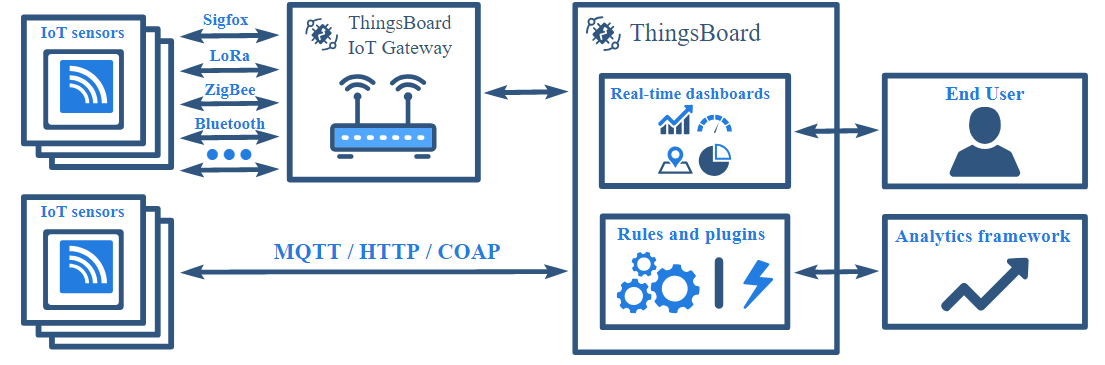
\includegraphics[width=\textwidth]{images/Khanh/Thingsboard/thingsboard_overall.png}
    \label{fig:thingsboard_overall}
\end{figure}

Với các tính năng ưu việt như thu thập dữ liệu từ xa, quản lý thiết bị và các báo động, Thingsboard cung cấp hơn 30 tiện ích có sẵn (Google map, Realtime chart, HTML tab, ...), cho phép tạo các bảng điều khiển (Dashboard) phong phú để hiển thị trực quan dữ liệu và điều khiển từ xa trong thời gian thực.

Bên cạnh đó, Thingsboardcho phép tạo các chuỗi quy tắc (Rule chains) kéo thả thân thiện để xử lý dữ liệu thiết bị dựa trên thuộc tính thực thể hoặc nội dung tin nhắn, tùy chỉnh logic xử lý phù hợp với các trường hợp sử dụng ứng dụng cụ thể. 



% !TEX root = ..\thesis.tex

\chapter{ Mô hình}
% vẽ sơ đồ hệ thống

Mô hình tổng quan của đề tài hình \ref{fig:general_chart}
\begin{figure}[H]
    \centering
    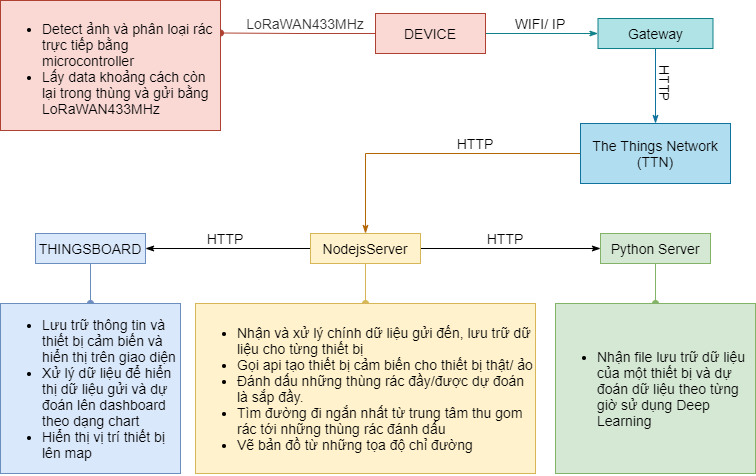
\includegraphics[width=\textwidth]{images/general_chart.png}
    \caption{Mô hình tổng quan}
    \label{fig:general_chart}
\end{figure}
Ở mô hình tổng quan đề tài, chúng tôi chia làm 2 phần, về thiết bị và về server.

\begin{itemize}
    \item Về thiết bị, tôi gắn 2 loại board và 2 ultrasonic sensor vào thùng rác để thực hiện 2 mục đích khác nhau, cụ thể:
        \begin{itemize}
            \item ESP32 camera AI Thinker, dùng vào mục đích chụp ảnh và phục vụ chức năng phân loại rác thải.
            \item  ESP32 Lora heltec, dùng trong mục đích thu thập data và gửi data cho server bằng công nghệ LoRaWAN.
            \item Ultrasonic sensor thực hiện nhiệm vụ đo độ dài khoảng trống còn lại trong thùng rác.
        \end{itemize}

    \item Về server, sử dụng Nodejs và Flask làm server cung cấp API, Thingsboard để làm giao diện hiển thị và một số server thứ ba khác, chức năng được mô tả cụ thể như sau:
        \begin{itemize}
            \item Nodejs Server là server nhận và xử lý chính dữ liệu, lưu trữ dữ liệu cho từng thùng rác. Từ đó, sử dụng dữ liệu để hiển thị, dự đoán và tìm đường đi tối ưu nhất để thu gom rác.
            \item Flask Server là server sử dụng Deep Learning để dự đoán dữ liệu được gửi từ Nodejs Server.
            \item Thingsboard là giao diện lưu trữ thông tin thùng rác, hiển thị dữ liệu theo nhiều dạng và vẽ đường đi trên bản đồ.
            \item Ngoài ra, còn sử dụng Thingsboard server hỗ trợ API thao tác đến Thingsboard và Mapbox server hỗ trợ API liên quan đến địa lý và đường đi.
        \end{itemize}
   

\end{itemize}


Hình \ref{fig:chart_smartbin} mô tả chi tiết về cấu tạo của thùng rác, và các thức hoạt động của 2 loại board được gắn bên trong thùng. 
\begin{figure}[H]
    \centering
    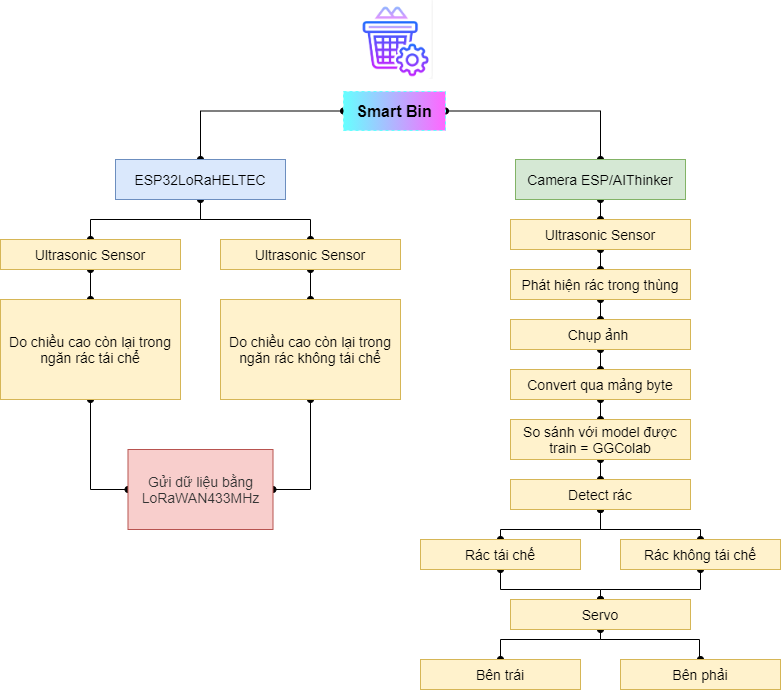
\includegraphics[width=\textwidth]{images/Chart_smartbin.png}
    \caption{Mô hình device}
    \label{fig:chart_smartbin}
\end{figure}


Mô hình server từ bước khởi tạo đến gửi dữ liệu \ref{fig:chart_server1}
\begin{figure}[H]
    \centering
    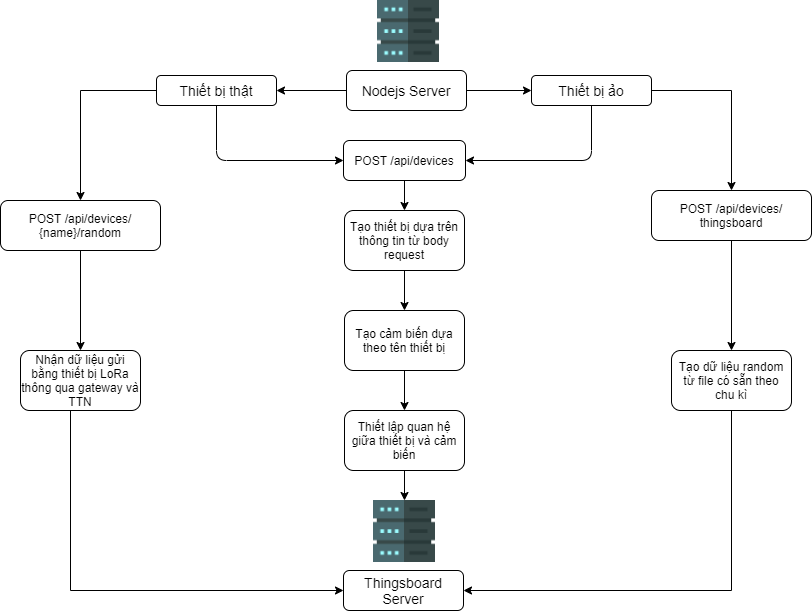
\includegraphics[width=\textwidth]{images/Khanh/Nodejs/Chart_server1.png}
    \caption{Mô hình server từ bước khởi tạo đến gửi dữ liệu}
    \label{fig:chart_server1}
\end{figure}

Mô hình server từ bước gửi dữ liệu đến xử lý bản đồ \ref{fig:chart_server2}
\begin{figure}[H]
    \centering
    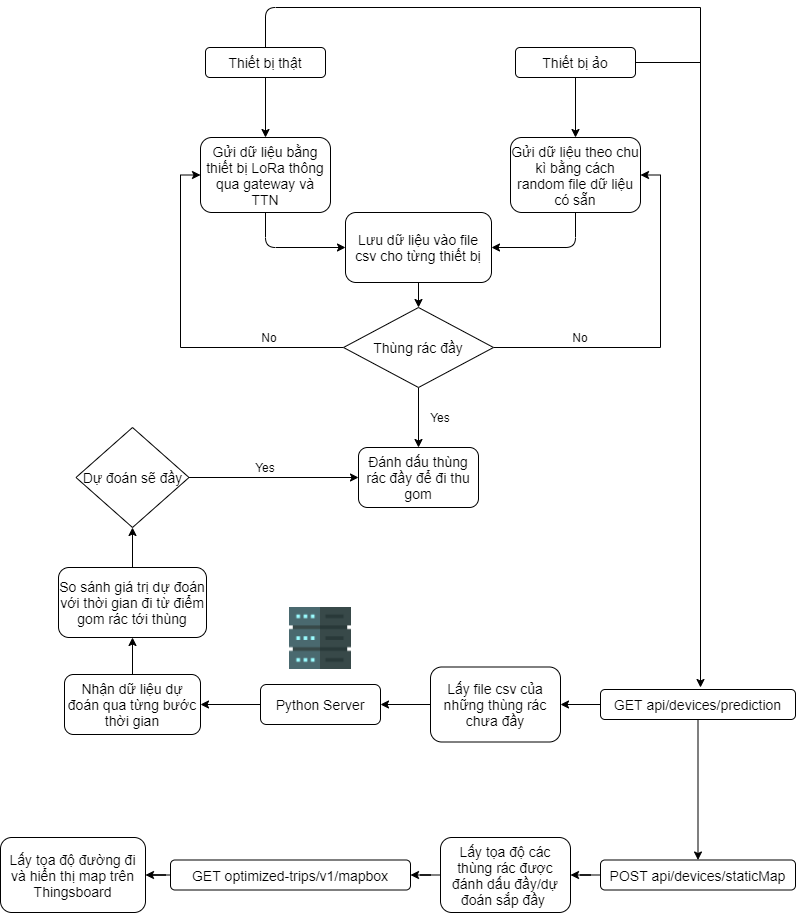
\includegraphics[width=\textwidth]{images/Khanh/Nodejs/Chart_server2.png}
    \caption{Mô hình server từ bước gửi dữ liệu đến xử lý bản đồ}
    \label{fig:chart_server2}
\end{figure}
% !TEX root = ..\thesis.tex


\chapter{XÂY DỰNG THIẾT BỊ TỰ ĐỘNG PHÂN LOẠI RÁC}



\section{Xây dựng model phân loại rác dựa trên CNN}
Trong mô hình thùng rác thông minh tự động phân loại rác, bài toán quan trọng được đặt ra trong mô hình này:
\begin{itemize}
    \item Đầu vào: Hình ảnh vật (rác) được bỏ vào thùng được chụp bằng camera của mạch ESP32 Cam AI Thinker với kích thước 96x96 pixels, có góc chụp từ trên xuống, với nền màu trắng, điều kiện ánh sáng tương đối đầy đủ. 
    \item Đầu ra: 1 số mang giá trị 0 hoặc 1 với giá trị 0 có nghĩa là loại rác không tái chế, và 1 có ý nghiã là rác tái chế. 
\end{itemize}

Để giải quyết bài toán: 
\begin{enumerate}
    \item Thiết kế kiến trúc mạng CNN phù hợp có thể triển khai vào thiết bị microcontroller.
    \item Thu thập dataset và tiến hành huấn luyện mạng CNN.
    \item Đánh giá khả năng phân loại ảnh rác của mạng CNN đã train.
\end{enumerate}

Trong thực tế, để hoàn thành bài toán đã đặt ra, ba bước đề cập ở trên được tiến hành không theo tuần tự mà phụ thuộc vào sự phát triển ở từng bước. Các vấn đề kỷ thuật chi tiết sẽ được trình bày ở các mục dưới đây.

\subsection{Tối ưu model để có thể chạy trên được chip nhúng ESP32}
% phần code 
\begin{figure}[ht]
    \centering
    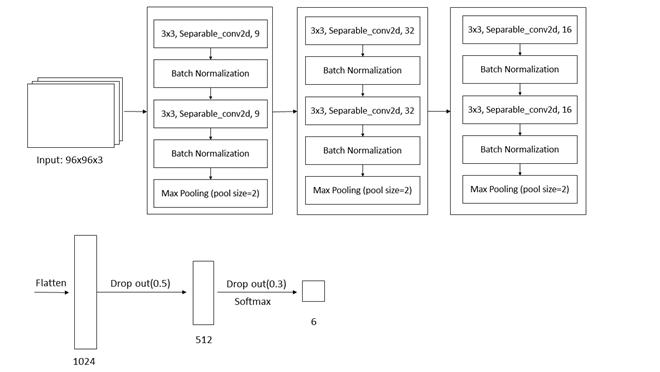
\includegraphics[width=\linewidth]{images/Quanh/ktmang.png}
    \caption{Minh họa kiến trúc mạng đã xây dựng}
    \label{fig:kientrucmang}
\end{figure}
% QUanhh viết r nè
% Do chip nhúng gì đó chỉ có bao nhiêu ram đó nên chúng tôi không thể xây dựng mô hình với trong số quá lớn và có chi phí tính toán cao được, nên chúng tôi sử dụng ...(thêm đoạn sau vô nè)
% Thêm dụ giảm kích thước của hình ảnh từ bao nhiêu đó xuống 96 * 96 nữa nà

Do sử dụng microcontroller cụ thể là board ESP32 camera AI Thinker, nên ram hỗ trợ rất khiêm tốn. chỉ có 4MB. nên chúng tôi không thể xây dựng mô hình với trọng số quá lớn và có chi phí tính toán cao được. Vì thế, chúng tôi chọn các sử dụng separable convolution thay cho lớp convolution thông thường để giảm bớt chi phí tính toán cho mạng. Ngoài ra ở lớp này, chúng tôi dùng regularization l2 để tránh overfitting và hàm kích hoạt relu – đây là hàm thường được sử dụng trong quá trình train model với dữ liệu dưới dạng ảnh. Chúng tôi cũng thêm các lớp batch normalization và drop out để tránh cho mô hình bị overfitting và loại bỏ sự kết nối chặt chẽ giữa các lớp fully connected. Tổng số tham số của mô hình là 532,161. Sau khi xây dụng mô hình, nhóm đã sử dụng optimization stochastic gradient descent với learning rate = 1e-4 và momentum = 0.8 để train mô hình. Cùng với việc giảm kích thước hình ảnh từ 512 × 384 pixels xuống còn 96x96 pixels để phù hợp với kích thước ram mà board hỗ trợ.

\subsection{Dataset và quá trình huấn luyện} % Giới thiệu về dataset ddùng để train và test 
% Dữ liệu được lấy từ cái gì đó quên oy, nhưng cái này nên thêm vô nha
% Kích thước của hình là ... không nhớ a
Chúng tôi dùng bộ dataset TrashNet \cite{trashnet} để train và test với kích thước 512x384.
Gồm 2527 hình thuộc 6 lớp với sự phận bố ở mỗi lớp:
 
Cardboard: 403

Glass: 501

Metal: 410

Paper: 594

Plastic: 482

Trash: 137
 
Dữ liệu được chia làm 2 phần theo tỉ lệ 80\% train và 20\% test.

Train: 2024

Test: 503

Sau đây là hình ảnh minh họa của 6 lớp cần phân loại như trên, được hiển thị ở bảng \ref{fig:trash_classification}.
\begin{table}[H]
    \centering
    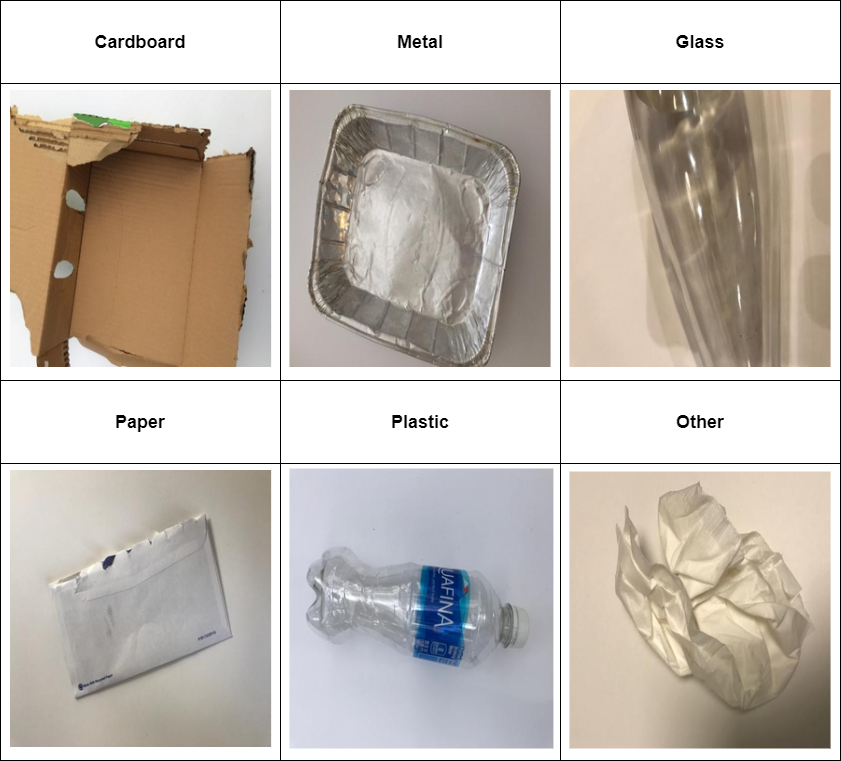
\includegraphics[width=\linewidth]{images/Quanh/Trash Classification.png}
    \caption{Phân loại hình ảnh trong bộ dataset}
    \label{fig:trash_classification}
\end{table}
% Nên lựa vài hình về data để thêm vô (nếu cần) hình nên có đủ 6 lớp cần phân loại
\subsection{Đánh giá hiệu quả của mạng CNN đã huấn luyện}

\subsubsection{Giới thiệu các độ đo tính hiệu quả của mạng CNN} % Các chỉ số để dánh gia model  %accuracy, F-score - Recall.
Chúng tôi sử dụng hai chỉ số là accuracy và F1-score để đánh giá model. Accuracy là tính tỉ lệ giữa số ảnh được dự đoán đúng và tổng số ảnh trong tập dữ liệu kiểm thử.

$Accuracy = \frac{TP+TN}{TP+TN+FP+FN}$

$Precision = \frac{TP}{TP+FP}$

$Recall = \frac{TP}{TP+FN}$

$F1 = \frac{2*Precision*Recall}  
{Precision+Recall} = \frac{2*TP}{2*TP+FP+FN}$
% Còn khúc giới thiệu F1 nữa cơ mà đang lười ghi công thức toán trong đây nha
% Khúc này thêm lý thuyết của hai cái chỉ số đó
\subsubsection{Kết quả  hiện thực được } % Kết quả  hiện thực được 
Kết quả train mô hình với 80 epoch
\begin{figure}[H]
    \centering
    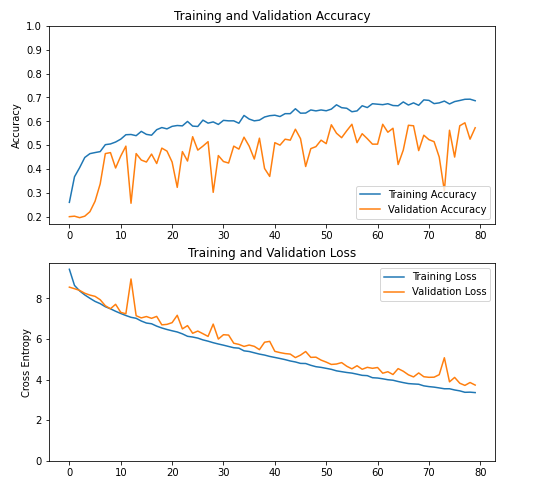
\includegraphics[width=\linewidth]{images/Quanh/graph.png}
    \caption{ Biểu đồ thể hiện loss và accuracy của mô hình trong quá trình train}
    \label{fig:graph}
\end{figure}
% Hai cái này nên chuyển thành dạng bảng, cơ mà đang lười chuyển
Accuracy cao nhất trên tập train là 0.6938 và trên tập test là 0.5938
Loss nhỏ nhất trên tập train là 3.3844 và trên tập test là 3.7116

Kết quả thử nghiệm mô hình trên tập test sau khi đã lưu mô hình tốt nhất từ quá trình train 
\begin{table}[H]
    \centering
    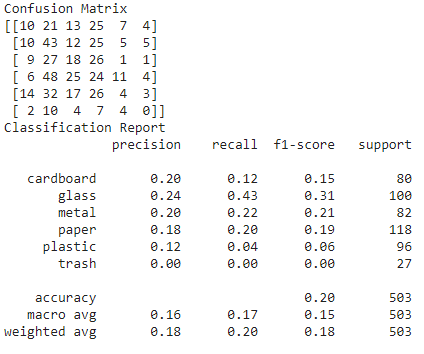
\includegraphics[width=\linewidth]{images/Quanh/matrix.png}
    \caption{Confusion matrix của model khi thử lại trên tập test}
    \label{fig:matrix}
\end{table}
Từ hình \ref{fig:matrix} ta có thể thấy accuracy và f1-score của mô hình còn khá thấp, tuy nhiên do mô hình được xây dựng chỉ có 532,161 tham số nên không đủ để phân loại chính xác các lớp được. Chúng tôi đã thử train thêm epoch nhưng mô hình dễ bị overfitting và kết quả khi in confusion matrix vẫn không thay đổi nhiều. Ngoài ra nếu tăng thêm trọng số thì không thể sử dụng model trên thiết bị được.


\section{Triển khai và kiểm thử mạng CNN phân loại rác trên thiết bị}
Sau khi model đã được train và evaluate kỹ lưỡng trên máy tính, công đoạn tiếp theo là build chương trình phân loại rác trên device dựa model đã train và thư viện TensorflowLite. 
Chương tình được build sẽ phải được kiểm thử để đảm bảo khả năng phân loại rác tương đương với khả năng phân loại của model đã được train trên ảnh từ PC.
% \subsection{Quy trình triển khai code phân loại rác trên device}
%Mô tả lại quy trình chuyển đổi từ file h5 của model sang file .cc để đưa vào code
%Đưa vào các đoạn code mẫu của tensorflowLite
\subsection{Quy trình thử nghiệm trên device}
%Đưa vào 2 đoạn code C++ và python và mô tả quy trình chạy:
%1. Device start và chờ tín hiệu "bắt đầu chụp ảnh" từ code python trên PC
%2. Mình bấm 1 nút trên PC, code python sẽ gửi tín hiệu "bắt đầu chụp ảnh" qua device
%3. Device chụp ảnh, lưu vào framebuffer của thư viện ESPCam rồi gửi qua cho code Python sau đó chờ tín hiệu "bắt đầu phân loại".
%4. Code python lưu ảnh xuống để thử nghiệm và sau đó gửi tín hiệu "bắt đầu phân loại" cho device.
%5. Device chạy đoạn code phân loại rác của tensorflowLite và gửi kết quả cho code Python sau đó quay lại chờ tín hiệu "bắt đầu chụp ảnh"
%6. Code python hiển thị kết quả phân loại ra cho mình kiểm tra sau đó lưu lại, chờ người dùng nhấn enter để bắt đầu lại quy trình kiểm tra
Để kiểm tra sự phân loại rác sau khi board ESP32 camera AI thinker hoàn thành việc chụp ảnh, tôi sử dụng 1 file python để laptop đóng vai trò như một server để nhận ảnh, detec ảnh, và trả kết quả detec. Việc trao đổi nhận ảnh từ board sang server sẽ sử dụng cable. 

Việc kiểm thử này phải đáp ứng được gần đúng với yêu cầu mà mô hình thực tế hình \ref{fig:chart_smartbin}. Quy trình thực hiện viêc kiểm tra sẽ bao gồm các bước sau:

Khi build file C để nạp code vào board thành công. Tiếp tục build file python để tạo server. Lưu ý vẫn giữ kết nối giữa board và laptop qua cable.

Để thay thế yêu cầu, khi ultrasonic sensor gặp vật cản sau đó khởi động chụp ảnh, thì trong môi trường kiểm tra. Tôi dùng một input được nhập từ bàn phím (nhấn enter) để thay thế bước trên. 
\begin{enumerate}
    \item Nhận input từ người dùng: khi nhấn enter: 
    \item send "1" đến board.
    \item nhận hình và kết quả dự đoán từ board .
    \item save hình vào local (cùng thư mục vs python, tên file là thời điểm nhận hình).
    \item show kết quả dự đoán trên console và bật app show ảnh ( đã save ở 4)
\end{enumerate}

\subsection{Kết quả phân loại khi chạy trên device}

%Đưa vào vài tấm hình được device chụp và kết quả phân loại tương ứng. 
%Sau đó chém gió là device chạy ra kết quả y chang như model đạt được ở mục trước
Một số hình ảnh được chụp từ thiết bị:
\begin{table}[H]
    \centering
    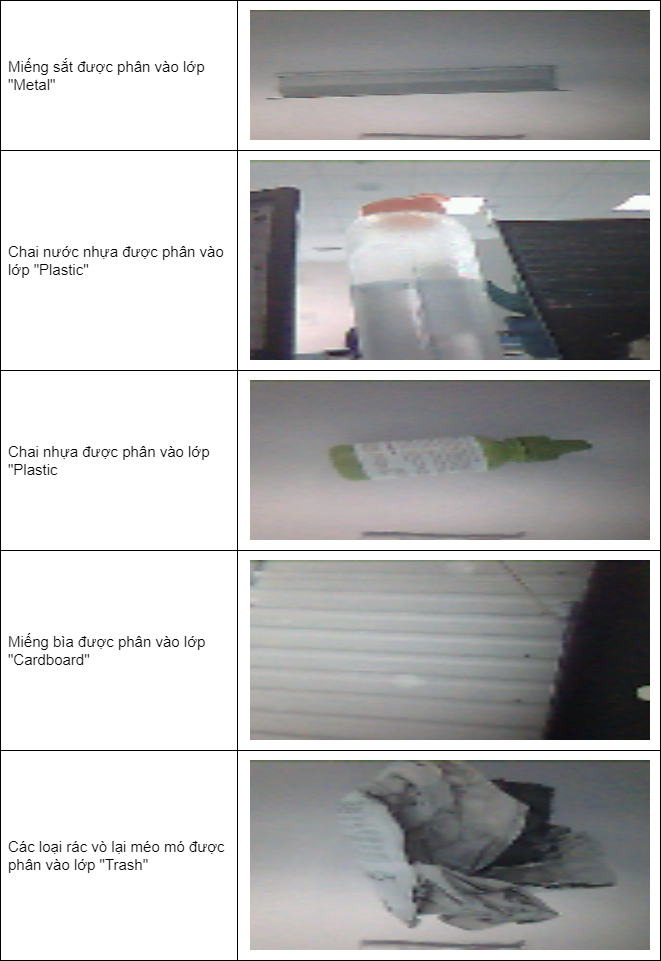
\includegraphics[width=\linewidth]{images/Quanh/Trash Result.png}
    \caption{Kết quả phân loại của một số hình ảnh}
    \label{fig:trash_result}
\end{table}

Tuy nhiên, do accuracy của model chỉ ở mức tương đối, và hình ảnh được train và hình ảnh được chụp từ thiết bị sẽ có thay đổi về màu sắc. Nên sẽ có một số loại rác bị detec sai. Dưới đây là các trường hợp sai trong quá trình kiểm thử.
\begin{table}[H]
    \centering
    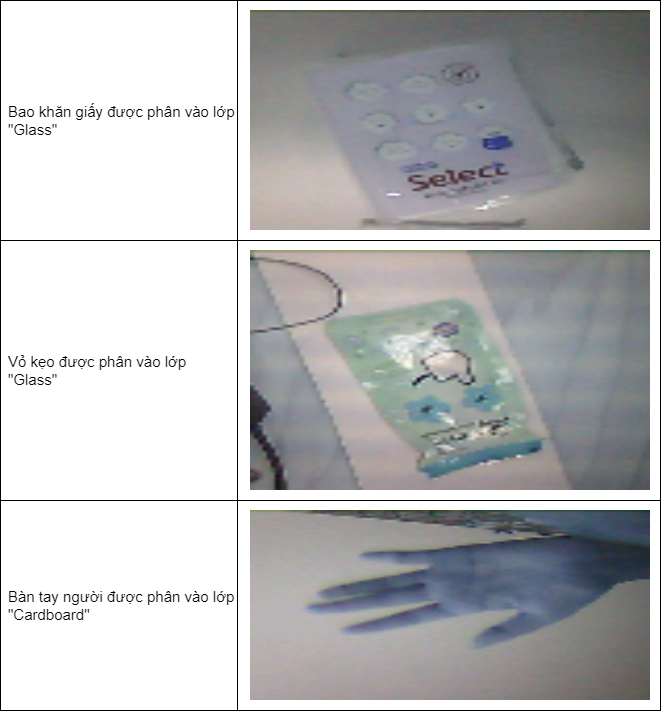
\includegraphics[width=\linewidth]{images/Quanh/Trash Failed.png}
    \caption{Một số kết quả sai trong quá trình phân loại}
    \label{fig:DWglass}
\end{table}

Như vậy, tuy có các trường hợp detec sai, nhưng có thể hình dung được mức độ đánh giá của model trong việc detec hình ảnh. Ví dụ như ở bảng \ref{fig:DWglass}, mặc dù đã bị detec sai lớp, nhưng có thể thấy, thủy tinh nói chung đều có tính chất phản ánh sáng, nên khi hình ảnh khi chụp 1 vật làm bằng thủy tinh sẽ có một độ bóng nhất định. Vì thế ở hình \ref{fig:DWglass} và \ref{fig:DWglass2} đều có tính chất phản ánh sáng như thủy tinh, nên thiết bị sẽ detec vào lớp "glass". Tương tự, các miếng bìa hầu hết trong tập dataset đều có các lằng vân nhấp nhô, và khi thiết bị chụp hình ảnh bàn tay người( hình \ref{fig:DWcardboar}), bàn tay cũng có các đường chỉ tay sâu, nên thiết bị sẽ detec vào lớp "cardboard".

\section{Setup Gateway}
\subsection{Access LG02}
Cấp nguồn điện cho gateway, sau đó dùng laptop để bật scan wifi, lúc này sẽ xuất hiện tên wifi : “dragino-168cb0”

Kết nối với wifi đó và truy cập địa chỉ IP: “10.130.1.1”, lúc này sẽ đến giao diện để configure gateway bằng cách nhập username và password như hình \ref{fig:gateway_configure}
\begin{figure}[H]
    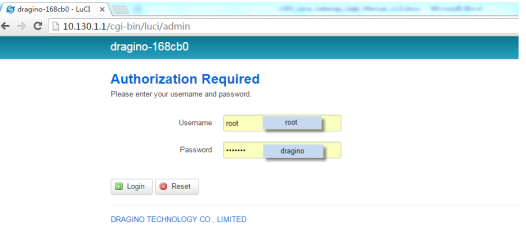
\includegraphics[width=\textwidth]{images/Quanh/Gateway_configure.png}
    \caption{Xác thực tại địa chỉ 10.130.1.1}
    \label{fig:gateway_configure}
\end{figure}

\subsection{Cài đặt network}
Truy cập Internet như Wifi Client theo các bước:
\begin{description}
    \item Bước 1: Network → Wireless, chọn radio0 và scan như hình \ref{fig:radio0_scan}
    \begin{figure}[H]
        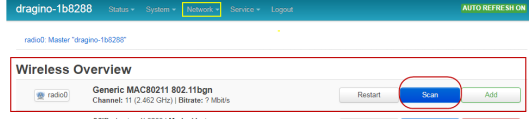
\includegraphics[width=\textwidth]{images/Quanh/Radio_scan.png}
        \caption{Scan mạng Wireless}
        \label{fig:radio0_scan}
    \end{figure}
    
    \item Bước 2: Chọn wifi và tham gia vào mạng, sau đó nhập mật khẩu và Submit như hình \ref{fig:join_password}
    \begin{figure}[H]
        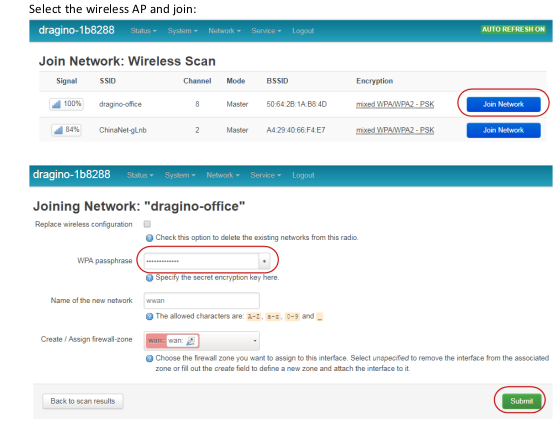
\includegraphics[width=\textwidth]{images/Quanh/Join_password.png}
        \caption{Tham gia vào wifi và nhập mật khẩu}
        \label{fig:join_password}
    \end{figure}
    \item Bước 3: Network → Wireless, chọn disable wifi mặc định của gateway như hình \ref{fig:disable_wifi}
    \begin{figure}[H]
        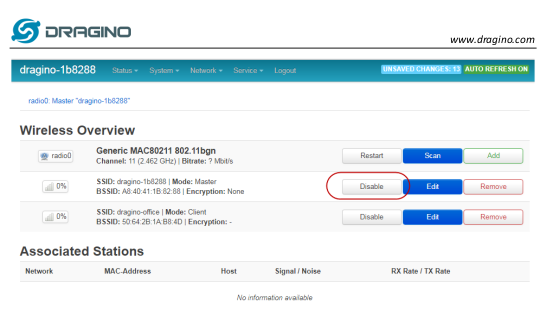
\includegraphics[width=\textwidth]{images/Quanh/Disable_wifi.png}
        \caption{Tắt wifi mặc định}
        \label{fig:disable_wifi}
    \end{figure}
\end{description}
(lưu ý, sau khi thực hiện bước 3, kết nối sẽ bị mất, nếu laptop kết nối wifi mặc định lúc nãy)

Trong trường hợp không thể truy cập địa chỉ 10.130.1.1 nữa, ta sử dụng cổng LAN để kết nối:
\begin{enumerate}
    \item Kết nối LAN Port
    \item Configure Ethernet port có địa chỉ IP là 172.31.255.253 và network 255.255.255.252.
    \item Dùng địa chỉ 172.31.255.254 để truy cập vào Web
\end{enumerate}


\subsection{Tạo gateway trên TTN Server}
\begin{description}
    \item Bước 1: Vào Service → LoRa → Lấy ID của Gateway như hình \ref{fig:get_gateway_id}
    \begin{figure}[H]
        \centering
        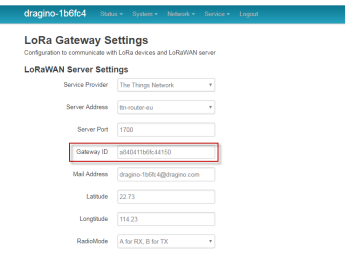
\includegraphics[width=\textwidth]{images/Quanh/Gateway_ID.png}
        \caption{Lấy ID của Gateway}
        \label{fig:get_gateway_id}
    \end{figure}
    \item Bước 2: Truy cập TTN: https://console.thethingsnetwork.org/gateways, giao diện hiển thị ở hình \ref{fig:gateway_console}
    \begin{figure}[H]
        \centering
        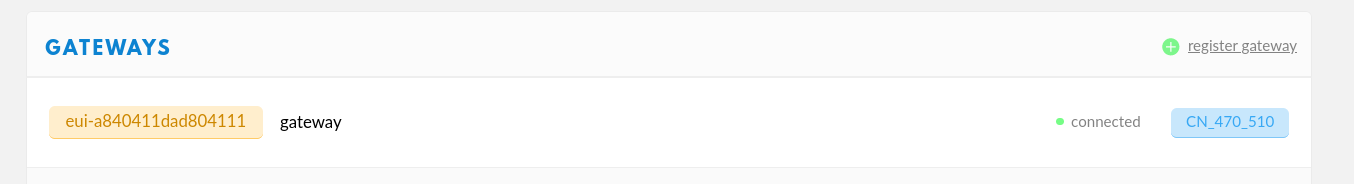
\includegraphics[width=\textwidth]{images/Quanh/Gateway_console.png}
        \caption{Giao diện Gateway đã được tạo (chưa connect)}
        \label{fig:gateway_console}
    \end{figure}
    \item Bước 3: Nhập ID vào Frequency plan tùy thuộc vào Gateway mà chọn cho phù hợp như hình \ref{fig:choose_gateway}, và kết quả được hiển thị ở hình \ref{fig:gateway_result} (nếu power on gateway thì status sẽ hiện "connected")
    \begin{figure}[H]
        \centering
        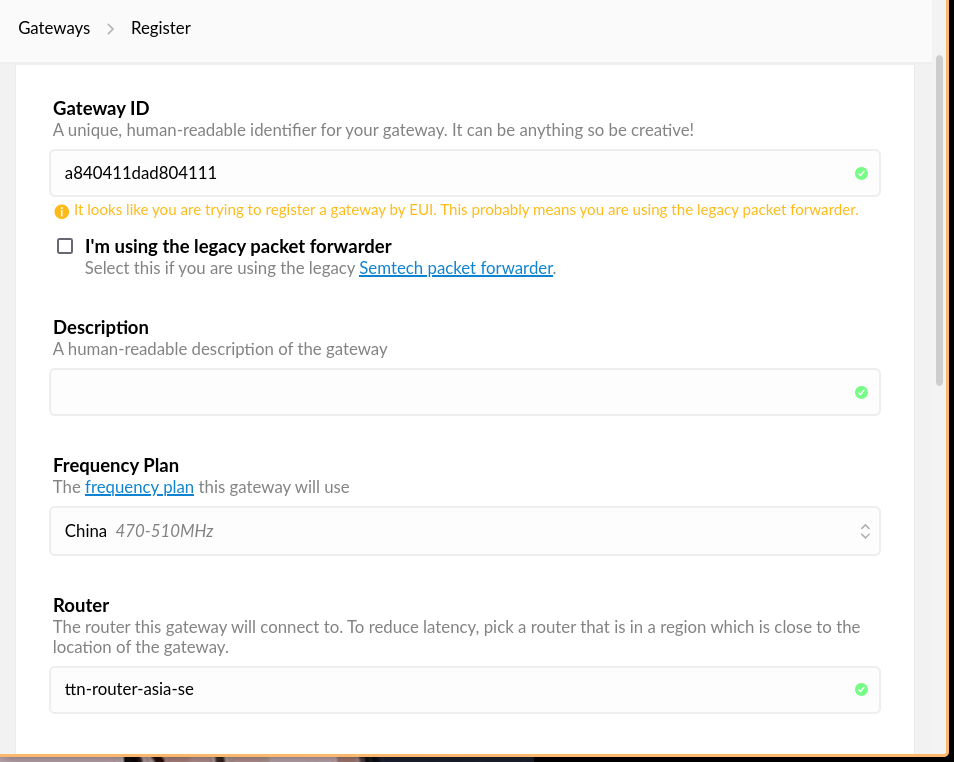
\includegraphics[width=\textwidth]{images/Quanh/Gateway_choose.png}
        \caption{Nhập ID vào Frequency plan}
        \label{fig:choose_gateway}
    \end{figure}
\end{description}
**do Gateway của nhóm sử dụng frequency 433Mhz nhưng The Things Network không hỗ trợ nên khi đăng kí sẽ là : china 470-510Mhz ( do tần số 433 trãi từng tần số 433 đến 510)

\subsection{Configure LG02 Gateway}
\begin{enumerate}
    \item Configure to LoRaWAN server qua các bước:
    \begin{description}
        \item Bước 1: Config LG02 với IoT Service là Lorawan/RAW forwarder, sau đó Save \& Apply
        \item Bước 2: Chọn Service Provider là The Things Network, Server Address là ttn-router-asia-se và Server Port là 1700
    \end{description}

    \item Configure LG02's RX frequency: Ở frequency 433Mhz, có 8 channel uplink nhưng nhóm chọn channel 433.175Mhz để end-device join vào, thông sô như hình \ref{fig:radio_config}
    \begin{figure}[H]
        \centering
        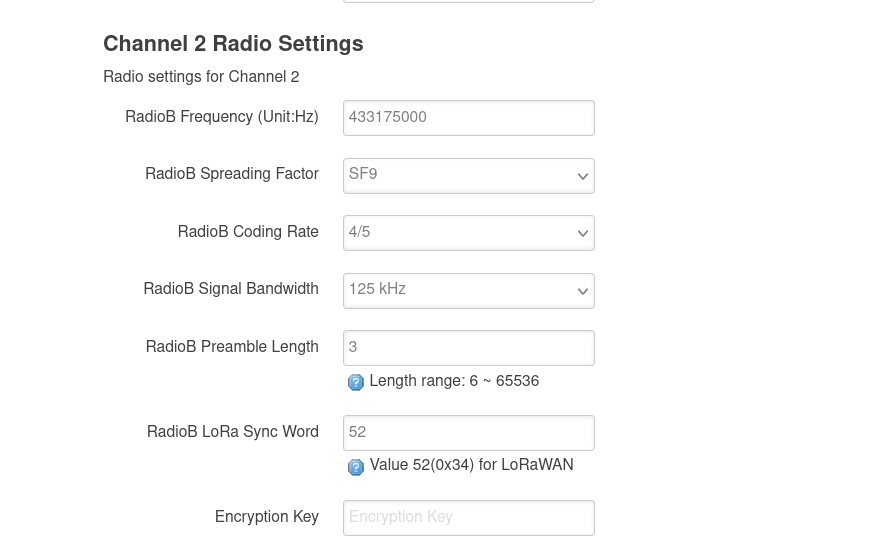
\includegraphics[width=\textwidth]{images/Quanh/Radio_config.png}
        \caption{Thông số configure}
        \label{fig:radio_config}
    \end{figure}
\end{enumerate}


\section{Setup End-Device}
\subsection{Thu gom rác}
Phần mềm sử dụng: Arduino IDE 1.8.2

Ngôn ngữ lập trình: C

Thiết bị Kit RF thu phát wifi Blue esp32 + Lora sx1278 oled Heltec.

\begin{description}
    \item Bước 1: Add lib esp32 từ link https://github.com/HelTecAutomation/Heltec\_ESP32 để thêm thư viện esp32 cho Arduino
    \item Bước 2: Add lib Lmic https://github.com/matthijskooijman/arduino-lmic để thêm vào thư viện Lmic cho Arduino
\end{description}

** Thư viện esp32 hỗ trợ hoạt động trên Heltech ESP32 develop framework.
** Thư viện Lmic cung cấp các giao tiếp LoRaWan ở classA và Class B. Tuy nhiên chỉ hỗ trợ ở band EU-868 và US 915. Nhưng thiết bị nhóm sử dụng là frequency 433Mhz nên cần sửa 1 số file để thiết bị có thể truyền data

Lúc này, có thể nạp code vào board như bình thường.

\subsection{Đăng kí trên TTN Server}
\begin{description}
    \item Bước 1: Tạo Application ID và handler, sau đó vào Devices → Register device → Điền Device ID  
    \item Bước 2: Sau khi đăng kí device thành công, The Things Network sẽ mặc định setup device join vào channel theo OTAA, nhưng nhóm chọn join theo ABP nên cần vào Setting → Activation method → ABP.
    
\end{description}



** ở phần này Payload Formats sẽ tùy thuộc vào code nạp vào end-device



\subsection{So sánh khi sử dụng Cayenne LPP và Custom}

Ta có bảng \ref{tab.comparison.Cayenne}

\begin{table}[H]
    \centering
    \caption{Loại rác} 
    \label{tab.comparison.Cayenne}
    \begin{tabular}{| m{6cm} | m{6cm} |}
        \hline
        Cayenne LLP & Custom \\

        \hline
        •	Không cần decoder (do thư viện Cayenne LPP đã có những quy định về code ở end-device) & •	Cần decoder để TTN hiển thị thông tin \\
        •	Khó hiển thị thêm các trường data từ sensor khác (Vì chỉ  hỗ trợ mặc định cho sensor nhiệt độ độ ẩm, các sensor khác phải qua pin Analog) & •	Có thể thêm nhiều sensor dễ dàng bằng code trên node, và chỉ cần cài đặt Payload formats trên TTN để hiển thị thông tin \\
        •	Mặc định payload & •	Có thể thay đổi Payload \\
        
        \hline
    \end{tabular}
\end{table}

Để chuyển data cho backend, cần cấu hình ở phần Integrations.



\subsection{Lưu ý khi nạp code cho node}

Vì sử dụng phương thức join vào server là ABP nên cần khai báo các thông tin cần thiết vào file *.ino để node có thể send data đến application server 

\begin{itemize}
    \item Device EUI, Network Session key và App Session key
    \item Để tối ưu việc truyền nhận từ node đến gateway,  nên disable các channels không cần thiết( chỉ enable channel đã khai báo ở RX của gateway)
\end{itemize}




% !TEX root = ..\thesis.tex



\chapter{SERVER}


\section{Nodejs Server}
\subsection{Giới thiệu tổng quát}
Nodejs là nền tảng phù hợp nhất đối với các ứng dụng nhận và xử lý dữ liệu realtime từ các thiết bị IoT. Vì thế, sử dụng Nodejs Server sẽ hỗ trợ tốt trong quá trình gửi dữ liệu realtime từ The Things Network (TTN) đến server thông qua HTTP và nhận, xử lý dữ liệu nhanh chóng nhờ vào cơ chế và các thư viện, gói mà Nodejs sở hữu. Bên cạnh đó, những thiết bị ảo cũng được lập trình với chức năng gần giống như các thiết bị IoT thật để tăng khả năng mở rộng của dự án khi chỉ có một số lượng nhỏ thiết bị thật cũng như hỗ trợ quá trình kiểm tra lỗi và hiển thị trực quan.

Ngoài việc xử lý nội bộ bên trong, Nodejs còn hỗ trợ kết nối với nhiều server bên thứ ba để tận dụng những API liên quan đến dự án như quản lý, hiển thị, địa lý, tiên đoán, ...

\subsection{Modules và packages được sử dụng}
Nodejs sử dụng kiến trúc Module để đơn giản hóa việc tạo ra các ứng dụng phức tạp, mỗi module chứa một tập các hàm chức năng khác nhau tùy vào mục đích của đối tượng. Bên ngoài những module tích hợp sẵn trong Nodejs, những module bên ngoài có thể được cài đặt vào nhờ vào trình quản lý package của Nodejs (npm). 

\begin{itemize}
    \item Những module tích hợp được sử dụng:
    \begin{itemize}
        \item http: biến server hoạt động như một máy chủ HTTP.
        \item fs: xử lý hệ thống tệp.
        \item os: cung cấp thông tin về hệ điều hành.
        \item cluster: chia nhiều luồng xử lý để tự động phân chia công việc.
    \end{itemize}
    \item Những module bên ngoài được sử dụng:
    \begin{itemize}
        \item dotenv: tải các biến môi trường từ tệp .env vào process.env.
        \item body-parser: phân tích cú pháp các phần thân nội dung yêu cầu đến trong phần mềm trung gian trước trình xử lý.
        \item express: framework được xây dựng trên nền tảng của Nodejs, cung cấp các tính năng mạnh mẽ để phát triển web hoặc mobile.
        \item cors: cơ chế cho phép nhiều tài nguyên khác nhau (fonts, Javascript, v.v…) của một trang web có thể được truy vấn từ domain khác với domain của trang đó.
        \item morgan: log trạng thái HTTP request.
        \item async-waterfall: hỗ trợ chạy một loạt các hàm không đồng bộ nối tiếp nhau, mỗi hàm chuyển kết quả của chúng cho các hàm tiếp theo.
        \item request: thực hiện HTTP request tới các server bên thứ ba.
        \item lodash: thư viện chuyên xử lý logic các nhóm đối tượng.
        \item random: trình tạo số ngẫu nhiên hỗ trợ nhiều phân phối phổ biến.
        \item csvtojson: chuyển đổi tệp .csv thành định dạng json hoặc mảng cột.
        \item moment: thư viện hỗ trợ xử lý thời gian.
        \item csv-write-stream: lưu trữ giá trị vào file csv thông qua luồng mã hóa CSV.
    \end{itemize}
\end{itemize}

Ngoài các module tích hợp và module bên ngoài, chương trình còn có một số module chức năng tự viết để giảm tải tính lặp lại khi lập trình.

\subsection{API}
Nodejs Server là trung tâm xử lý chính luồng dữ liệu gửi đến, cung cấp những một loạt những API liên quan đến khởi tạo thiết bị, cảm biến thật và ảo, nhận và xử lý dữ liệu sau đó lưu vào database. Ngoải ra còn có API gọi tới Python server để xử lý Deep Learning cho những thùng chưa đầy, và API tìm đường đi tối ưu nhất đến các thùng đã đầy hoặc dự đoán sắp đầy.

Sau đây là tất cả API mà server cung cấp với bản mô tả chi tiết từng luồng chức năng:
\begin{itemize}

    \item Xử lý chung:
    \begin{itemize}
        \item POST /api/devices: Tạo và cài đặt thùng rác, cảm biến
        \begin{description}
            \item Mô hình luồng xử lý được mô tả tổng quát ở hình \ref{fig:create_device} 
        \end{description}
        \begin{itemize}
            \begin{figure}[H]
                \centering
                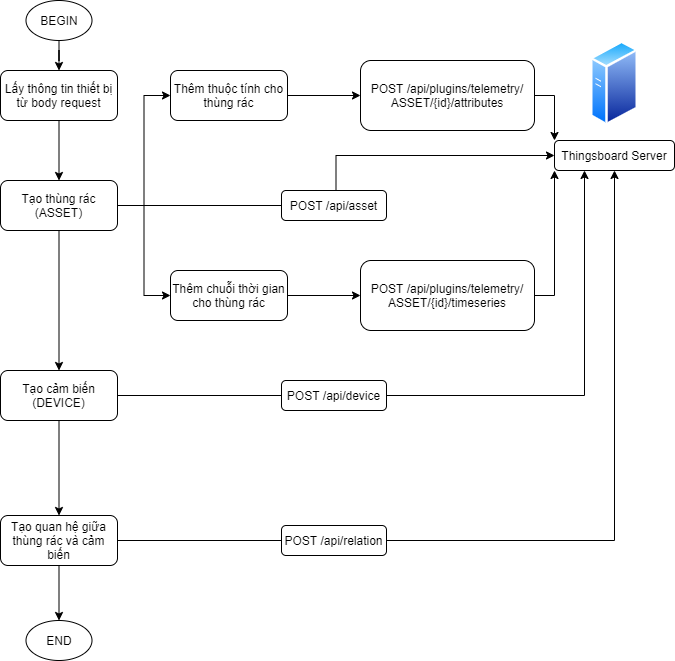
\includegraphics[width=\textwidth]{images/Khanh/Nodejs/Server_Create_Stimulate_Device.png}
                \caption{Sơ đồ miêu tả mô hình khởi tao thiết bị và cảm biến}
                \label{fig:create_device}
            \end{figure}
            \item Trước khi tạo một thùng rác thật/ảo mới cũng phải điền đầy đủ những thông tin sau trong body:
            \begin{itemize}
                \item name (string): tên thùng rác.
                \item type (string): loại thùng rác.
                \item address (string): địa chỉ của thùng, nếu không có thì sẽ sử dụng API Geocoding từ Mapbox nhận vào tọa độ của thùng để định vị địa chỉ.
                \item latitude (double): kinh độ.
                \item longitude (double): vĩ độ.
                \item nonrecycleHeight (double): chiều cao ngăn không tái chế.
                \item recycleHeight (double): chiều cao ngăn tái chế. 
            \end{itemize} 
            \item Sau khi gửi body request như trên, một loạt hàm sẽ được chạy dựa trên cơ chế waterfall, sử dụng request để gọi API khởi tạo từ Thingsboard. Những API từ Thingsboard đều có JWT để bảo mật route, khi sử dụng phải cần có token đăng nhập lấy từ API POST /api/auth/log. Token sau đó được gắn vào header ở dạng 'Bearer \{token\}' ở trường 'X-Authorization'. Nếu không có token thì mọi API sẽ trả về status 401 unauthorized.
            \begin{enumerate}
                \item POST /api/asset để tạo mới thùng rác, nhận vào \{name, type\} của thùng rác. Nếu status trả về là 201 tức là tạo thùng rác thành công, còn 404 là báo lỗi trùng tên thùng rác. ID thùng rác trả về sẽ được lưu trữ.
                \item POST /api/device để tạo mới cảm biến, nhận vào \{name, type\} của cảm biến. Vì trong thùng luôn chứa hai cảm biến siêu âm để phân loại rác tái chế và không tái chế nên tên cảm biến sẽ được chuẩn hóa theo dạng '\{name\}{\_}\{function\}', ví dụ: '\{name\}{\_}taiche' và '\{name\}{\_}khongtaiche'. Nếu status trả về 201 tức là tạo cảm biến thành công, còn 404 là báo lỗi trùng tên cảm biến. ID cảm biến trả về sẽ được lưu trữ.
                \item POST /api/plugins/telemetry/ASSET/\{id thùng rác\}/\{attributes || timeseries\} để thêm các thuộc tính hoặc giá trị theo thời gian cho thùng, những thuộc tính mặc định bao gồm \{address, latitude, longitude, recycleHeight, nonrecycleHeight\} còn giá trị thời gian thì có mức rác 2 ngăn, giá trị tiên đoán và message thông báo. Nếu trường đã có thì sẽ thay đổi giá trị trường đó. Nếu status 201 tức là thêm thành công, 404 là báo lỗi thiếu dữ liệu.
                \item POST /api/relation để tạo quan hệ một nhiều giữa thùng rác và cảm biến, nhận vào body dạng \{from: \{type: 'ASSET', id: \{id thùng rác\}\}, to: \{type: 'DEVICE', id: \{id cảm biến\}\}\}. Nếu status 201 tức là thành công, còn 404 là thiếu dữ liệu hoặc id không tồn tại.
                \item Sau khi thao tác thành công, thông tin thùng rác sẽ được lưu lại dưới server để xử lý dữ liệu và dự đoán.
            \end{enumerate}
        \end{itemize}

        \item GET /api/devices/prediction: Xử lý dự đoán mức rác cho những thùng rác chưa đầy, được gọi vào 1 giờ trước khi thu gom rác.
        \begin{description}
            \item Mô hình luồng xử lý được mô tả tổng quát ở hình \ref{fig:predict_empty_bin} 
        \end{description}
        \begin{enumerate}    
            \begin{figure}[H]
                \centering
                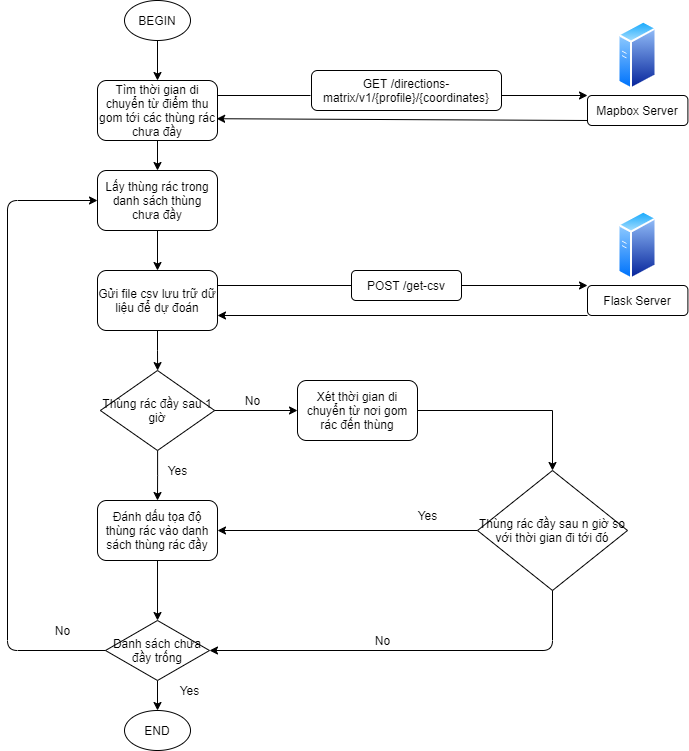
\includegraphics[width=\textwidth]{images/Khanh/Nodejs/Server_Predict_Empty_Bin.png}
                \caption{Sơ đồ miêu tả mô hình gửi dữ liệu tiên đoán và kiểm tra mức rác}
                \label{fig:predict_empty_bin}
            \end{figure}
            \item Lấy tọa độ của những thùng rác chưa đầy, sau đó định dạng theo kiểu chuỗi '\{lng{\_}nơigomrác\},\{lat{\_}nơigomrác\};\{lng{\_}thùng1\},\{lat{\_}thùng1\};\{lng{\_}\newline thùng2\},\{lat{\_}thùng2\} \dots\ '.
            \item Gọi API từ Mapbox GET /directions-matrix/v1/\{profile\}/\{coordinates\}?\newline sources\&annotations\&access{\_}token để lấy ma trận khoảng cách hoặc thời gian di chuyển giữa nhiều điểm. Những params và query được mô tả chi tiết như sau:
            \begin{itemize}
                \item profile (params): cấu hình ID phương tiện, giá trị bao gồm "driving", "walking", "cycling" và "driving-traffic". 
                \item coordinates (params): danh sách tọa độ \{kinh độ, vĩ độ\} được phân tách bằng dấu chấm phẩy.
                \item sources (query): đánh chỉ tọa độ làm điểm nguồn tới tất cả tọa độ còn lại. 
                \item annotations (query): dùng để chỉ định kết quả trả về, giá có thể có là "duration" (thời lượng) hoặc "distance" (khoảng cách) hoặc cả hai ngăn cách bằng dấu phẩy.
                \item access{\_}token (query): token key được cung cấp bởi Mapbox
            \end{itemize}
            \item Kết quả trả về sẽ theo dạng ma trận 1xn (n là số thùng chưa đầy) [0, n1, n2, n3, ...], mỗi phần tử là thời gian di chuyển từ điểm nguồn tới từng tọa độ trong \{coordinates\}.
            \item Duyệt qua những thùng rác chưa đầy, khi file .csv lưu trữ dữ liệu quá ít thì sẽ không dự đoán, còn lại thì sẽ gửi file .csv qua Python Server để dự đoán mức rác vào một giờ sau (giờ gom rác).
            \item Kết quả trả về là một mảng một chiều, mỗi phần tử là lượng rác được dự đoán sau \{index + 1\} giờ. Nếu phần tử 0 (lượng rác vào lúc thu gom) lớn hơn hoặc bằng 90\% chiều cao thùng tức là thùng đó dự đoán sẽ đầy sau một giờ và sẽ được đánh dấu thùng rác đầy.
            \item Đối với những thùng rác dự đoán chưa đầy vào một giờ, thì ta xét trong thời gian từ lúc bắt đầu tới khi đến được thùng rác, thùng có đầy không. Bằng cách lấy thời gian di chuyển đến thùng đó so với các khoảng giờ i (max=3), nếu thời gian nằm trong khoảng giờ i, thì sẽ lấy lượng rác dự đoán sau i + 1 giờ. 
            \item Lấy kết quả dự đoán so với 90\% của thùng, nếu được dự đoán sẽ đầy thì sẽ được đánh dấu vào những thùng đầy.
        \end{enumerate}

        \item GET /api/devices/static-map
        \begin{description}
            \item Mô hình luồng xử lý được mô tả tổng quát ở hình \ref{fig:get_map} 
        \end{description}
        \begin{enumerate}    
            \begin{figure}[H]
                \centering
                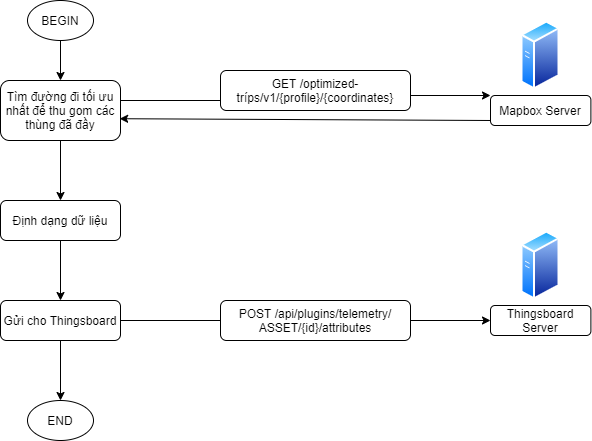
\includegraphics[width=\textwidth]{images/Khanh/Nodejs/Server_Get_Map.png}
                \caption{Sơ đồ miêu tả luồng xuất mảng tọa độ đường đi tối ưu tới thùng rác đầy}
                \label{fig:get_map}
            \end{figure}
            \item Lấy tọa độ của những thùng rác đầy, sau đó định dạng theo kiểu chuỗi '\{lng{\_}nơigomrác\},\{lat{\_}nơigomrác\};\{lng{\_}thùng1\},\{lat{\_}thùng1\};\{lng{\_}\newline thùng2\},\{lat{\_}thùng2\} \dots\ '.
            \item Gọi API từ Mapbox GET /optimized-trips/v1/\{profile\}/\{coordinates\}?\newline language\&roundtrip\&geometries\&steps\&access{\_}token để lấy ma trận khoảng cách hoặc thời gian di chuyển giữa nhiều điểm. Những params và query được mô tả chi tiết như sau:
            \begin{itemize}
                \item profile (params): cấu hình ID phương tiện, giá trị bao gồm "driving", "walking", "cycling" và "driving-traffic". 
                \item coordinates (params): danh sách tọa độ \{kinh độ, vĩ độ\} được phân tách bằng dấu chấm phẩy.
                \item language (query): định dạng ngôn ngữ trả về ở văn bản hướng dẫn.
                \item steps (query): trả về chi dẫn từng chặng chi tiết.
                \item roundtrip (query): cho biết tuyến đường có phải là khứ hồi hay không.
                \item geometries (query): định dạng kiểu trả về, giá trị bao gồm "geojson", "polyline", "polyline6".
                \item access{\_}token (query): token key được cung cấp bởi Mapbox.
            \end{itemize}
            \item Kết quả trả về là một mảng tọa độ chỉ đường đi đến tất cả thùng rác đầy, sau đó định dạng lại theo dạng [[\{lat1\},\{lng1\}],[\{lat2\},\{lng2\}],...].
            \item Gửi kết quả định dạng lên Thingsboard thông qua API POST /api/plugins\newline/telemetry/ASSET/\{id\}/attribute với id của nơi gom rác được tạo sẵn để hiển thị đường đi lên bản đồ Thingsboard.   
        \end{enumerate}
    \end{itemize}

    \item Xử lý dữ liệu cảm biến của thiết bị ảo và thiết bị thật:
    \begin{itemize}  
        \item Mô hình luồng xử lý được mô tả tổng quát ở hình \ref{fig:random_telemetry}
        \begin{figure}[H]
            \centering
            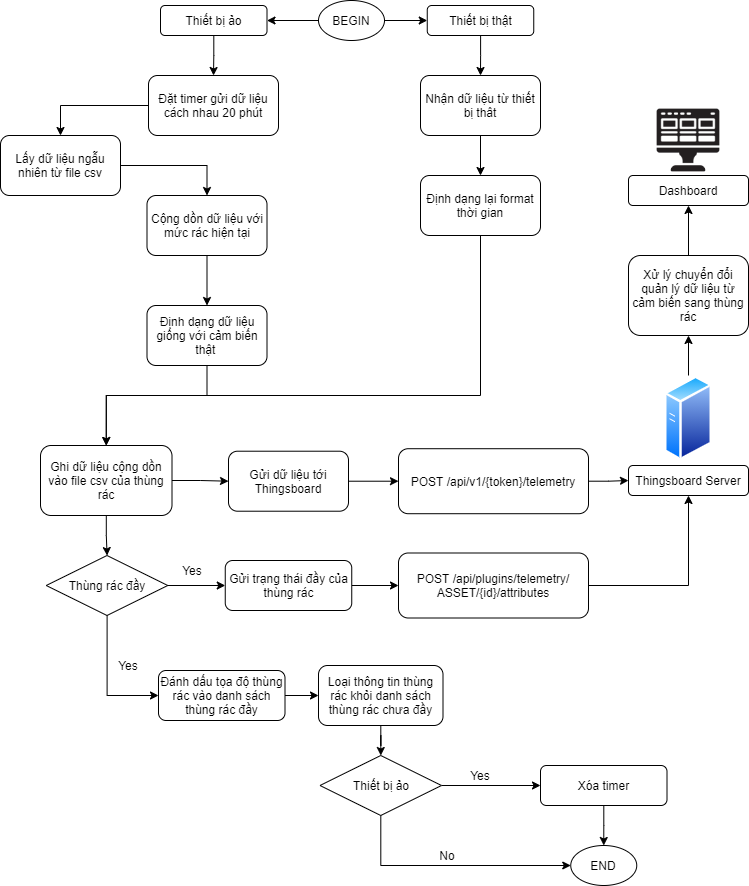
\includegraphics[width=\textwidth]{images/Khanh/Nodejs/Server_Random_Telemetry.png}
            \caption{Sơ đồ miêu tả luồng tạo dữ liệu giả cho thiết bị ảo}
            \label{fig:random_telemetry}
        \end{figure}   
        \begin{enumerate}
            \item Với thiết bị thật (POST /api/TTN/telemetry): 
            \begin{itemize}
                \item Những thiết bị thật sẽ gửi dữ liệu thông qua API này với định dạng được tạo từ TTN được mô tả trong bảng ... 
                ... 
                \item Vì dữ liệu được gửi bằng cảm biến thật nên không cần thay đổi định dạng của chúng, ...
            \end{itemize}
            \item Với thiết bị ảo (POST /api/devices/\{deviceName\}/random):
            \begin{itemize}
                \item Tiến hành tạo ngẫu nhiên dữ liệu của thùng rác có tên \{deviceName\}, cài đặt timer bằng cách setInterval với khoảng thời gian là 120.000ms (20 phút/1 lần).
                \item Dữ liệu được lấy ngẫu nhiên trong file random.csv với giá trị tái chế và không tái chế ngẫu nhiên từ 0 tới 13.
                \item Khởi tạo mức delta bằng 0, khi thùng rác chưa đầy ta lấy delta cộng với giá trị ngẫu nhiên đó và lấy chiều cao thùng rác trừ cho tổng giá trị sẽ ra được giá trị thật của cảm biến. Thực hiện đến khi nào thùng rác đầy thì giá trị ngẫu nhiên sẽ bằng 0 và khi đó giá trị sẽ dừng ở mức cao nhất của thùng rác.  
                \item Định dạng dữ liệu giống với format payload\_fields của thiết bị thật, đối với thời gian thì sử dụng moment để lấy thời gian thực. 
            \end{itemize}
            \item Sau bước định dạng dữ liệu của 2 loại thiết bị, lưu dữ liệu vào file .csv của từng thùng với tên "\{deviceName\}\_deltaHeight.csv", bên trong file bao gồm các cột timestamp (thời gian), recycleData (dữ liệu tái chế) và nonrecycleData (dữ liệu không tái chế). Đồng thời dữ liệu sẽ được gửi lên Thingsboard, chuyển đổi thực thể và hiển thị lên giao diện theo dạng biểu đồ đường.
            \item Khi thùng rác đã đầy, ta sẽ gửi thông báo đến Thingsboard để hiển thị màu sắc, cùng lúc đó, đánh dấu thùng rác đó vào danh sách các thùng rác đầy và xóa khỏi danh sách các thùng rác chưa đầy. Đối với thiết bị ảo, sẽ dừng timer để giảm tải công việc cho server.
        \end{enumerate}
    \end{itemize}

\end{itemize}

\section{Python Server}
\subsection{Giới thiệu tổng quát}
Python là sự ưu tiên hàng đầu khi được lựa chọn ngôn ngữ cho các dự án liên quan đến AI. Vì thế sử dụng Python làm một server thứ ba cung cấp API xử lý chính các vấn đề về dự đoán lượng rác, sau đó việc trả kết quả về bên server chính để xử lý tiếp sẽ nhanh và hiệu quả hơn việc xử lý Deep Learning tại Nodejs.

Flask là framework được lựa chọn để xây dựng server vì tính năng hỗ trợ các yêu cầu RESTful và dễ dàng triển khai và tương tác với các server khác. Chức năng chính của server được mô tả tổng quát là cung cấp một API nhận và chuyển một tệp dạng .csv lưu trữ chuỗi thời gian đa biến thành các supervised learning. Sau đó sẽ chia tập lớn thành tập train và tập test, rồi đưa vào mô hình mạng LTSM để dự báo lượng rác sau từng khoảng thời than. 

\subsection{Modules và packages}
Flask có cung cấp thư viện mở rộng flask-restful hỗ trợ cho việc xây dựng các RESTful API một cách nhanh chóng, khuyến khích các phương pháp hay nhất với thiết lập tối thiểu. Ngoài ra, việc xử lý Deep Learning cần sử dụng một số thư viện quan trọng sau:

\begin{itemize}
    \item tensorflow: thư viện mã nguồn mở dùng cho tính toán số học sử dụng đồ thị luồng dữ liệu, xử lý dựa trên sự thay đổi của dữ liệu.
    \item sklearn: thư viện cung cấp một tập các công cụ xử lý các bài toán máy học và mô hình thống kê.
    \item numpy: thư viện lõi của Python, hỗ trợ cho việc tính toán dãy số và ma trận nhiều chiều với tốc độ xử lý nhanh.
    \item math: thư viện hỗ trợ các hàm toán học tiêu chuẩn C.
    \item matplotlib: thư viện hỗ trợ vẽ đồ thị hai chiều, ba chiều mạnh mẽ.
    \item pandas: thư viện hỗ trợ xử lý và phân tích các dữ liệu có cấu trúc (dạng bảng, đa chiều, ...) và dữ liệu chuỗi thời gian nhanh, mạnh mẽ và linh hoạt.
\end{itemize}

\subsection{API}
Server cung cấp 1 API GET /get-csv với luồng dữ liệu được mô tả tổng quát ở hình \ref{fig:python_general}

\begin{figure}[H]
    \centering
    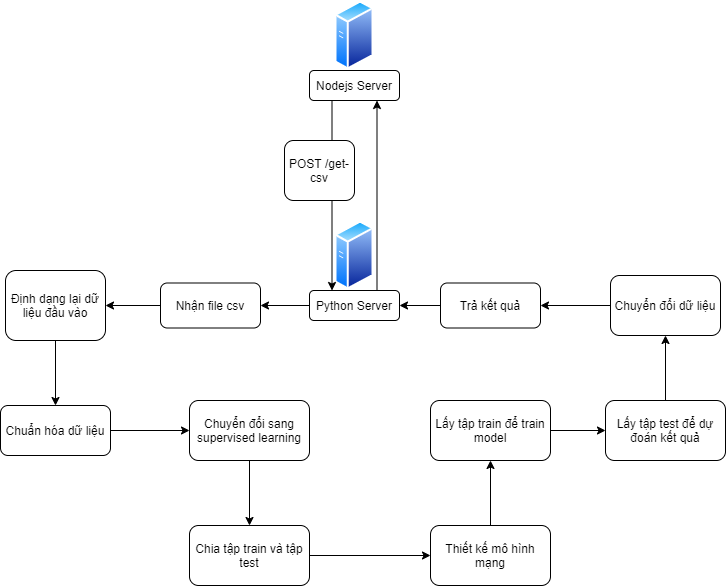
\includegraphics[width=\textwidth]{images/Khanh/Python/Python_general.png}
    \caption{Sơ đồ mô tả tổng quát mô hình Deep Learning dự đoán lượng rác}
    \label{fig:python_general}
\end{figure}

Luồng dữ liệu được mô tả chi tiết như sau:

\begin{enumerate}
    \item Server nhận vào một tệp .csv được gửi từ Nodejs Server, bao gồm các cột [thời gian, lượng rác tái chế, lượng rác không tái chế]. 
    \item Tách riêng 2 cột tái chế và không tái chế thành 2 mảng 2 chiều riêng biệt dưới dạng [[a1],[a2],[a3],...].
    \item Chuyển các mảng thành dạng mảng Numpy và định dạng kiểu float32 để thuận tiện sử dụng.
    \item Chuẩn hóa các mảng bằng MinMaxScaler giúp thuật toán dễ dàng xử lý hơn.
    \item Quy định lấy 75\% chuỗi dữ liệu để làm tập train và phần còn lại để làm tập test. Chuyển đổi tất cả các tập sang supervised learning với số time\_step tự quy định (số time\_step trước đó được sử dụng để dự đoán giá trị ở time\_step tiếp theo).
    \item Kết quả trả về là một mảng 2 chiều có shape là (số lượng dữ liệu, time\_steps). Reshape các tập train input lại thành kiểu (samples, timeseries, features) để đưa vào mô hình dự đoán.
    \item Xây dựng mô hình mạng Stacked LSTM như bảng \ref{tag.lstm.model}
    \begin{table}[H]
        \centering
        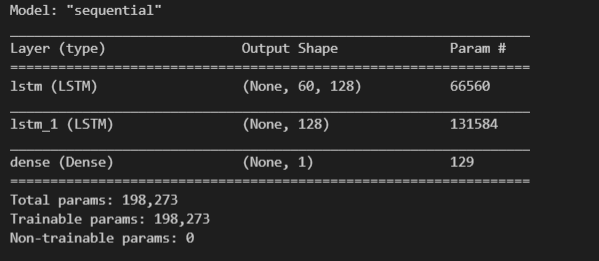
\includegraphics[width=\textwidth]{images/Khanh/Python/LSTM Model.PNG}
        \caption{Tổng quan mô hình mạng LSTM}
        \label{tag.lstm.model}
    \end{table}
    bằng cách tạo một mô hình Sequential và thêm nhiều layer vào trong, cụ thể là 2 LSTM layers và 1 Dense layer với các tham số. Sau đó model sẽ compile với các tham số để train model (loss, optimizer, metrics) và fit data vào để train (bao gồm tổng cộng 198.273 params có thể train được).
    \item Ta lấy \{time\_step\} phần tử cuối từ tập test với t là thời điểm của giá trị cuối cùng để dự đoán dữ liệu ở thời điểm t+1 ... và tiếp đó chạy vòng lặp để dự đoán dữ liệu ở t+2, t+3, t+4 ... bằng cách lấy giá trị dự đoán ở t+1 cho vào mảng, dịch phần tử đầu tiên ra khỏi mảng và tiếp tục dự đoán t+2.
    \item Trả kết quả dự đoán mức rác tái chế và không tái chế về Nodejs Server để tiếp tục xử lý. 
\end{enumerate}

\subsection{Đánh giá dữ liệu}
Chúng tôi gửi một tệp .csv của một thùng rác có chuỗi dữ liệu thu thập mỗi 20 phút vào tháng 6 với tổng 2161 dữ liệu như hình \ref{tab:CSV_structure}:
\begin{figure}[H]
    \centering
    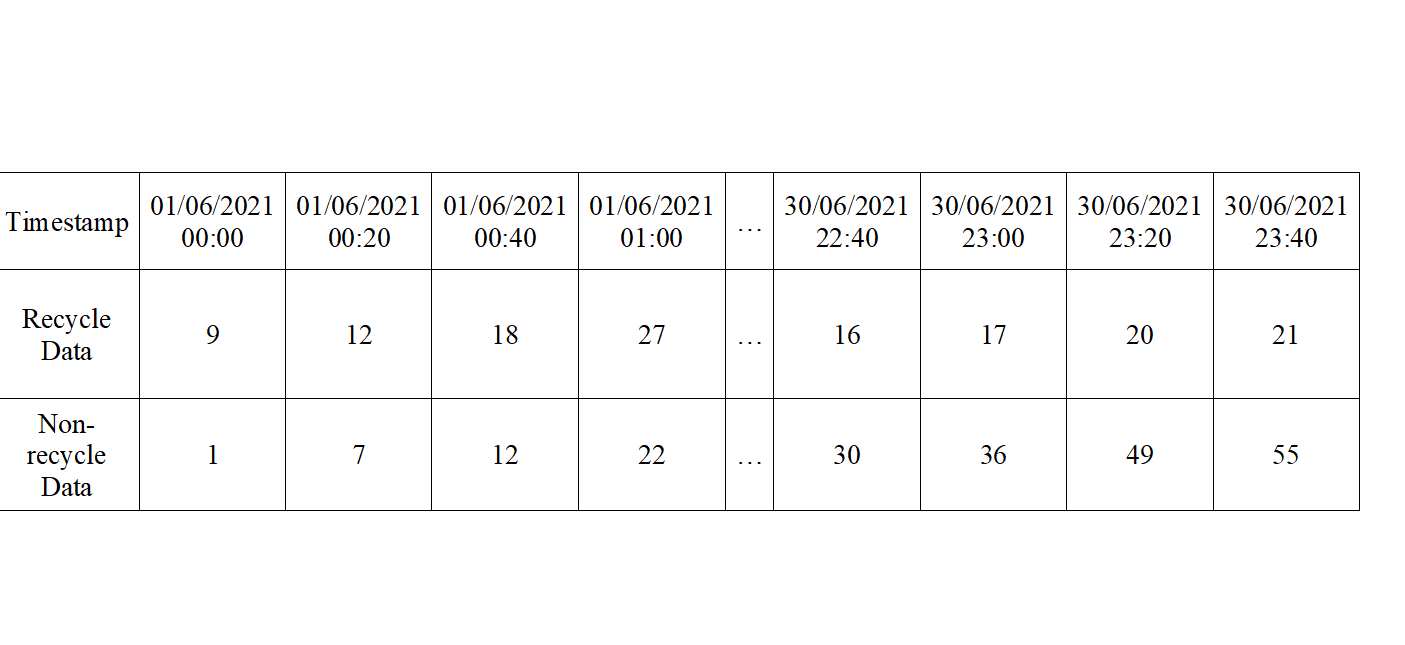
\includegraphics[width=\textwidth]{images/Khanh/Python/CSV_Structure.PNG}
    \caption{Cấu trúc file CSV}
    \label{tab:CSV_structure}
\end{figure}

hiển thị dưới dạng biểu đồ hình \ref{fig:CSV_plot_chart}
\begin{figure}[H]
    \centering
    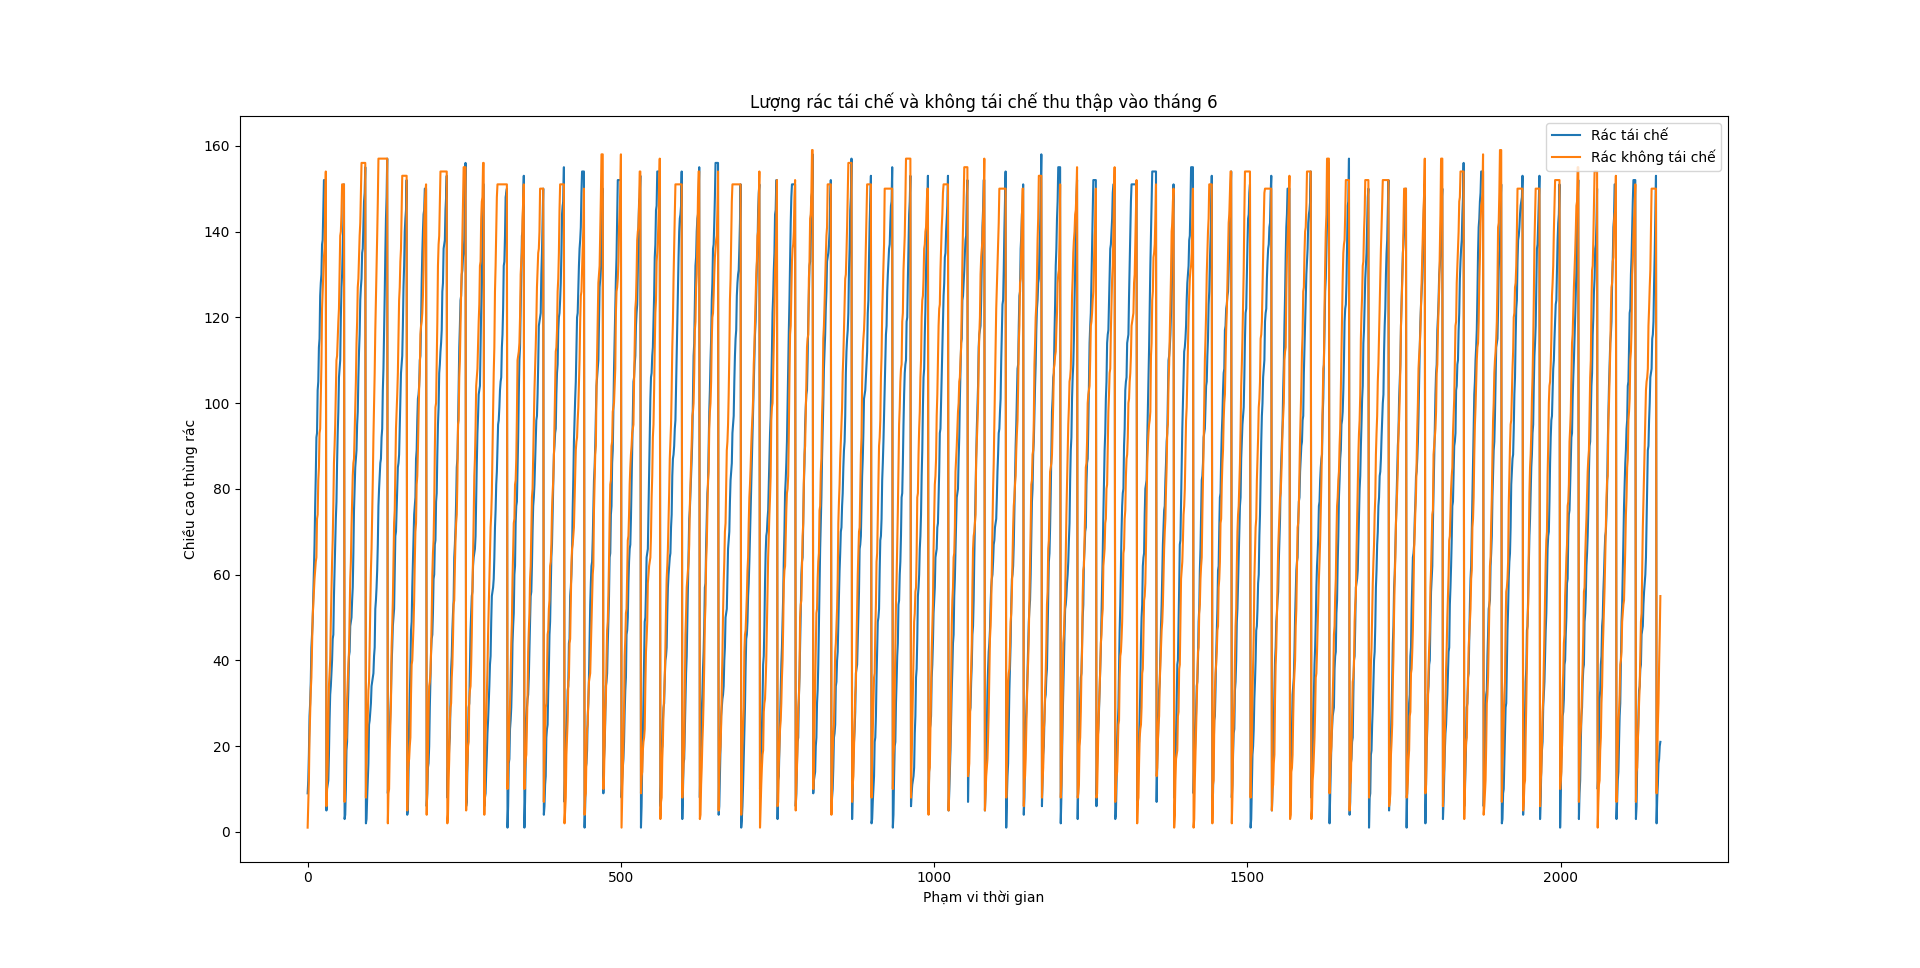
\includegraphics[width=\textwidth]{images/Khanh/Python/CSV_Plot_Chart.png}
    \caption{Biểu đồ lượng rác tái chế và không tái chế thu thập vào tháng 6}
    \label{fig:CSV_plot_chart}
\end{figure}

\begin{description}
    \item timestamp: mốc thời gian
    \item recycle data: lượng rác tái chế
    \item non-recycle data: lượng rác không tái chế
\end{description}

Tập dữ liệu được chuyển thành supervised learning với time\_steps là 60 (tức là lấy dữ liệu 20 tiếng trước để dự đoán) và chia thành 75\% cho tập train (1620) và phần còn lại (541) cho tập test.

Sau khi train mô hình, chúng tôi đánh giá model bằng chỉ số loss để đo tỉ lệ chênh lệch giữa tập dữ liệu thực và tập dữ liệu model dự đoán.

Kết quả train mô hình với 20 epochs cho thấy loss nhỏ nhất trên tập train là 0.05242335423827171 và trên tập test là 0.047845833003520966, được biểu diễn ở biểu đồ \ref{fig:loss_chart}  
\begin{figure}[H]
    \centering
    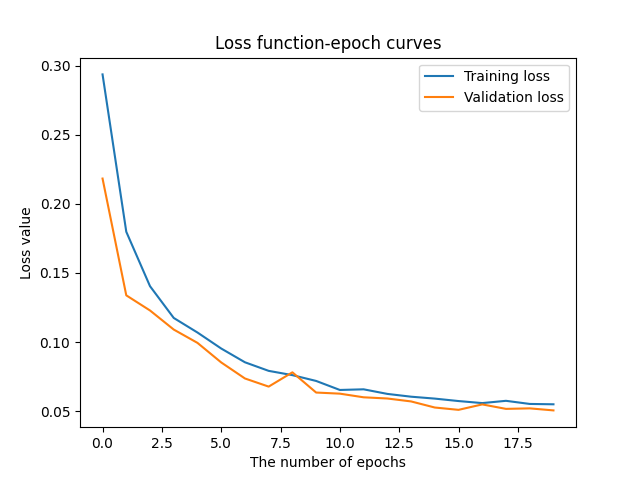
\includegraphics[width=\textwidth]{images/Khanh/Python/Loss_Chart.png}
    \caption{Giá trị Train loss và Val loss}
    \label{fig:loss_chart}
\end{figure}

Sau đó chúng tôi sử dụng tập test để dự đoán và so sánh kết quả dự đoán với dữ liệu thực như hình \ref{fig:test_recycle_actual_prediction} cho mức rác tái chế và hình \ref{fig:test_non_recycle_actual_prediction} cho mức rác không tái chế với kết quả RMSE và MSE cho tập test mức rác tái chế là 97.511 và 86.812, RMSE và MSE cho tập test mức rác không tái chế là 104.531 và 93.270.
\begin{figure}[H]
    \centering
    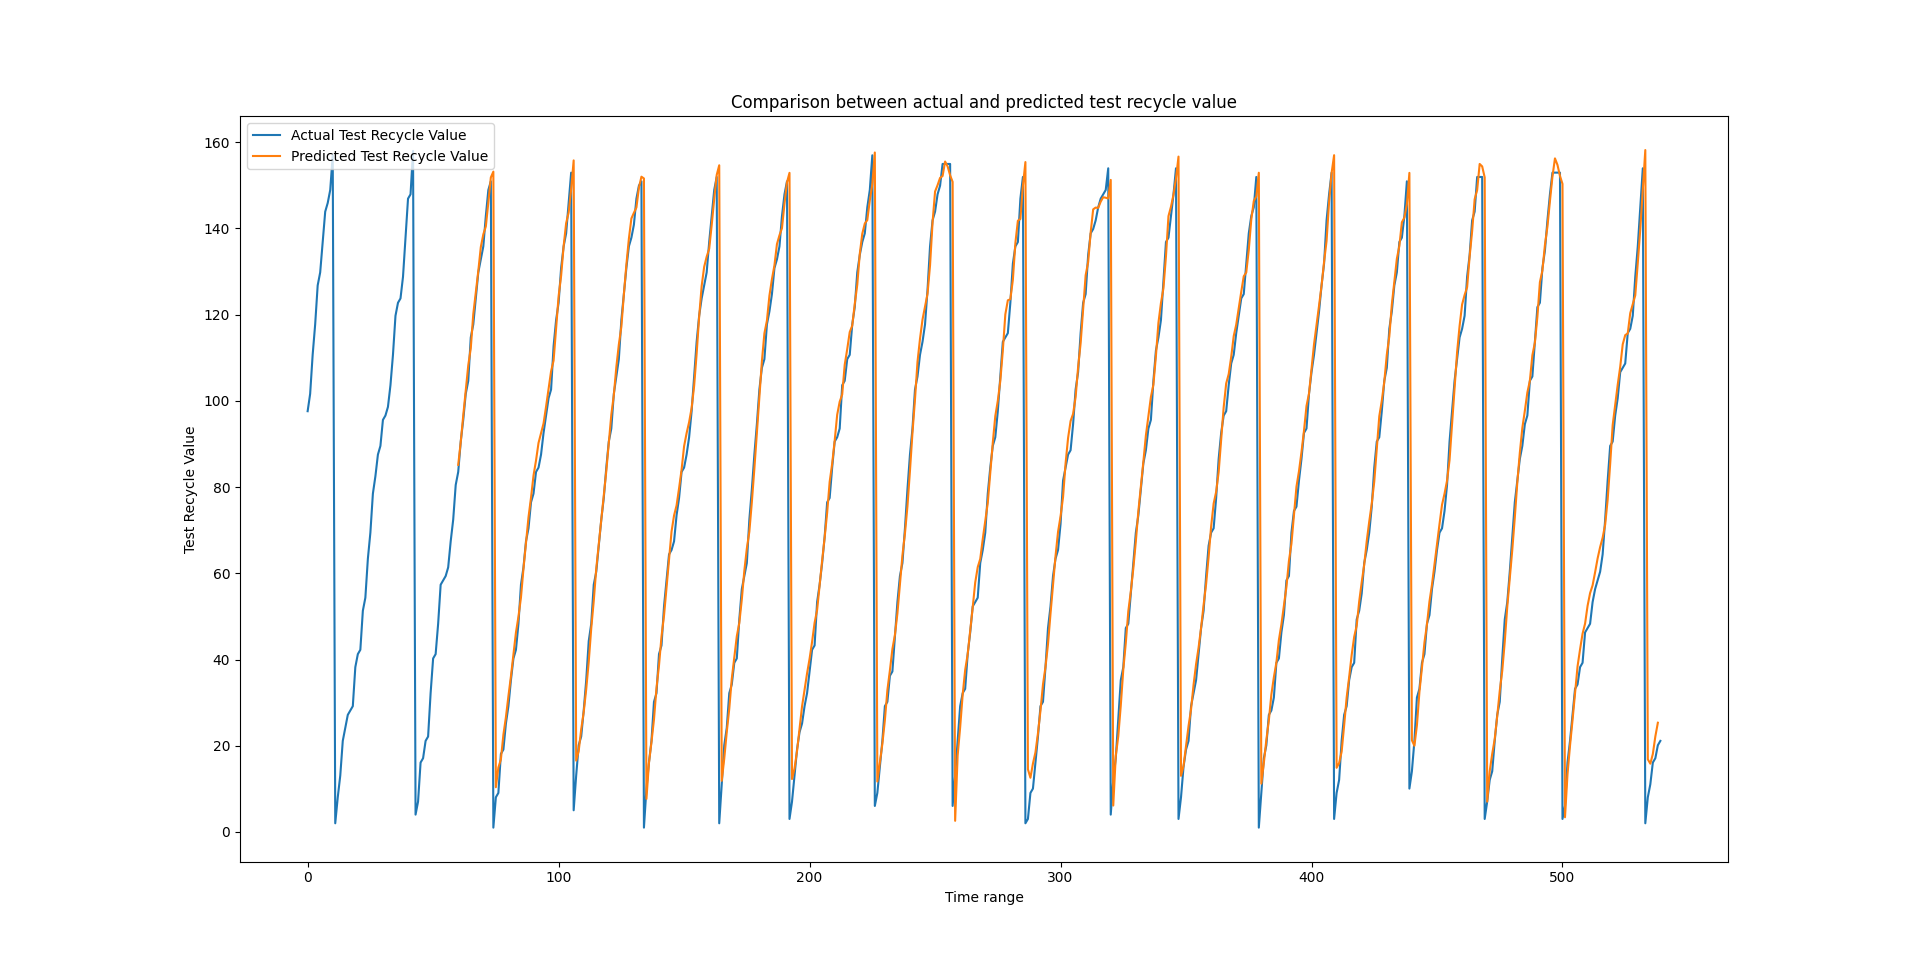
\includegraphics[width=\textwidth]{images/Khanh/Python/Recycle_Test_Chart.png}
    \caption{So sánh actual với predicted của tập test tái chế}
    \label{fig:test_recycle_actual_prediction}
\end{figure}
\begin{figure}[H]
    \centering
    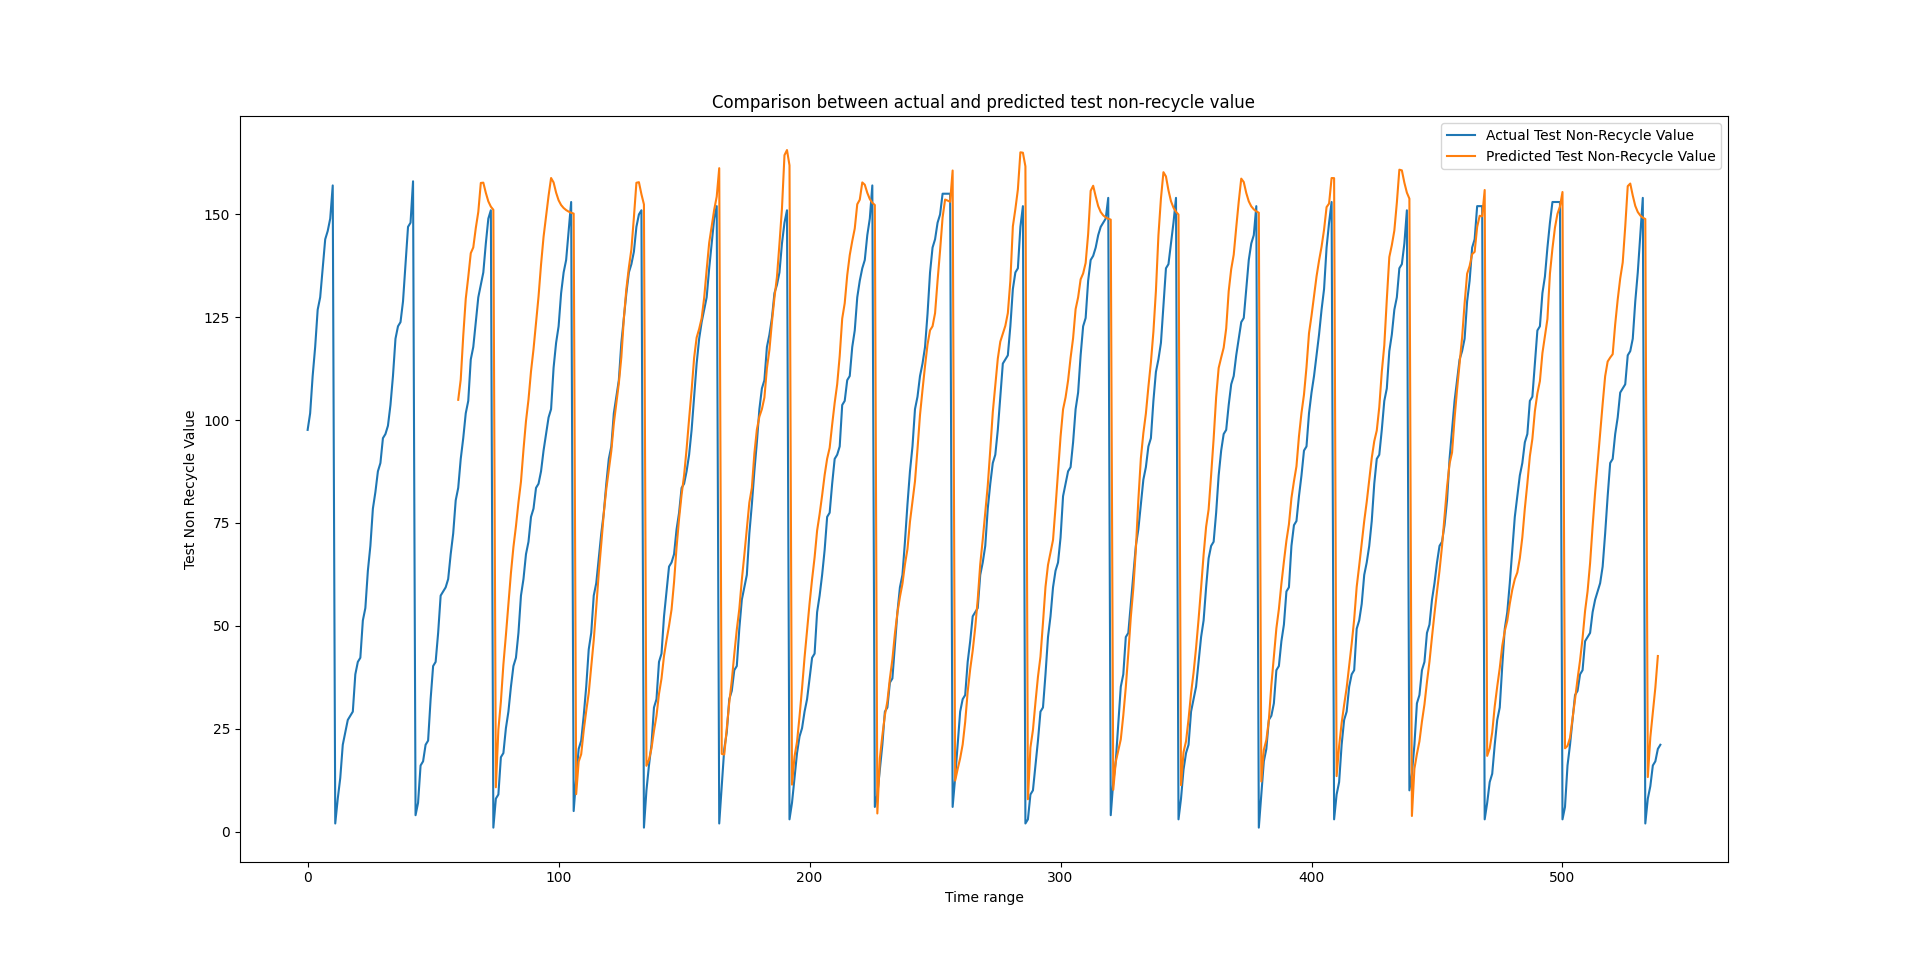
\includegraphics[width=\textwidth]{images/Khanh/Python/Non-Recycle_Test_Chart.png}
    \caption{So sánh actual với predicted của tập test không tái chế}
    \label{fig:test_non_recycle_actual_prediction}
\end{figure}

Ở bước cuối cùng chúng tôi sử dụng model để dự đoán mức rác vào 12 time\_steps (4 tiếng tiếp theo), kết quả hiển thị như hình \ref{fig:final_result}
\begin{figure}[H]
    \centering
    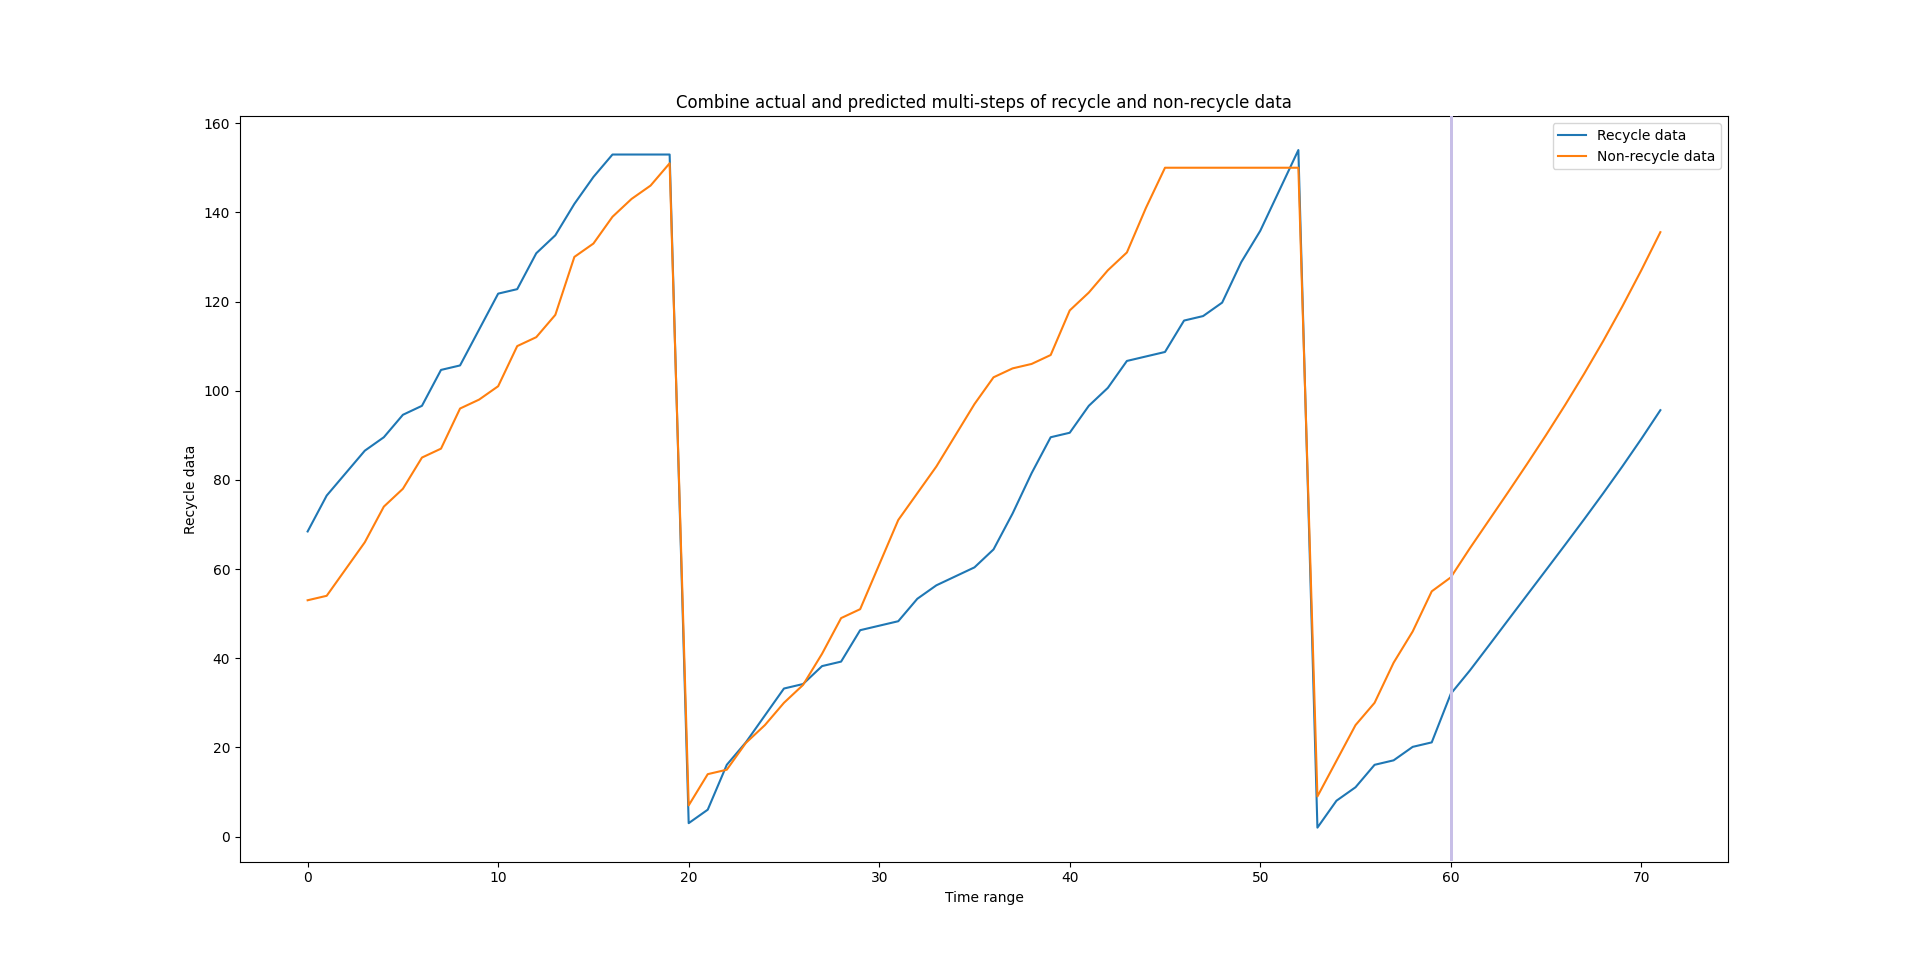
\includegraphics[width=\textwidth]{images/Khanh/Python/Final_results.png}
    \caption{Biểu đồ mức rác tái chế và không tái chế sau 4 tiếng tiếp theo}
    \label{fig:final_result}
\end{figure}

\section{Thingsboard}
\subsection{Giới thiệu tổng quát}
Việc xử lý dữ liệu ở server vẫn chưa đủ, thông tin dữ liệu của thùng rác cần được hiển thị cho cả admin và người dùng quan sát. Vì thế, Thingsboard vừa được sử dụng như một Frontend đáp ứng việc này đồng thời cung cấp một doc cung cấp những API để hỗ trợ đưa thông tin lên giao diện.

Chúng tôi sử dụng bản demo của Thingsboard cho dự án để giảm bớt thời gian cài đặt cho bản Localhost và chi phí cho bản Premium, tuy vậy những tính năng mà bản demo mang lại vẫn đáp ứng đầy đủ những yêu cầu mà dự án cần. 

\subsection{Assets và Devices}
Cả asset và device đều là một thực thể của Thingsboard, ở trong dự án này asset được quy định là thùng rác và device được quy định là cảm biến của thùng rác đó. Những thực thể có thể được tạo thủ công trên giao diện hoặc tự động bằng Thingsboard API, và sẽ được lưu trữ tại database PostgreSQL.

Thingsboard cung cấp 2 tab bao gồm danh sách tất cả asset và device đã tạo như hình \ref{fig:asset_general} và \ref{fig:device_general}.
\begin{figure}[H]
    \centering
    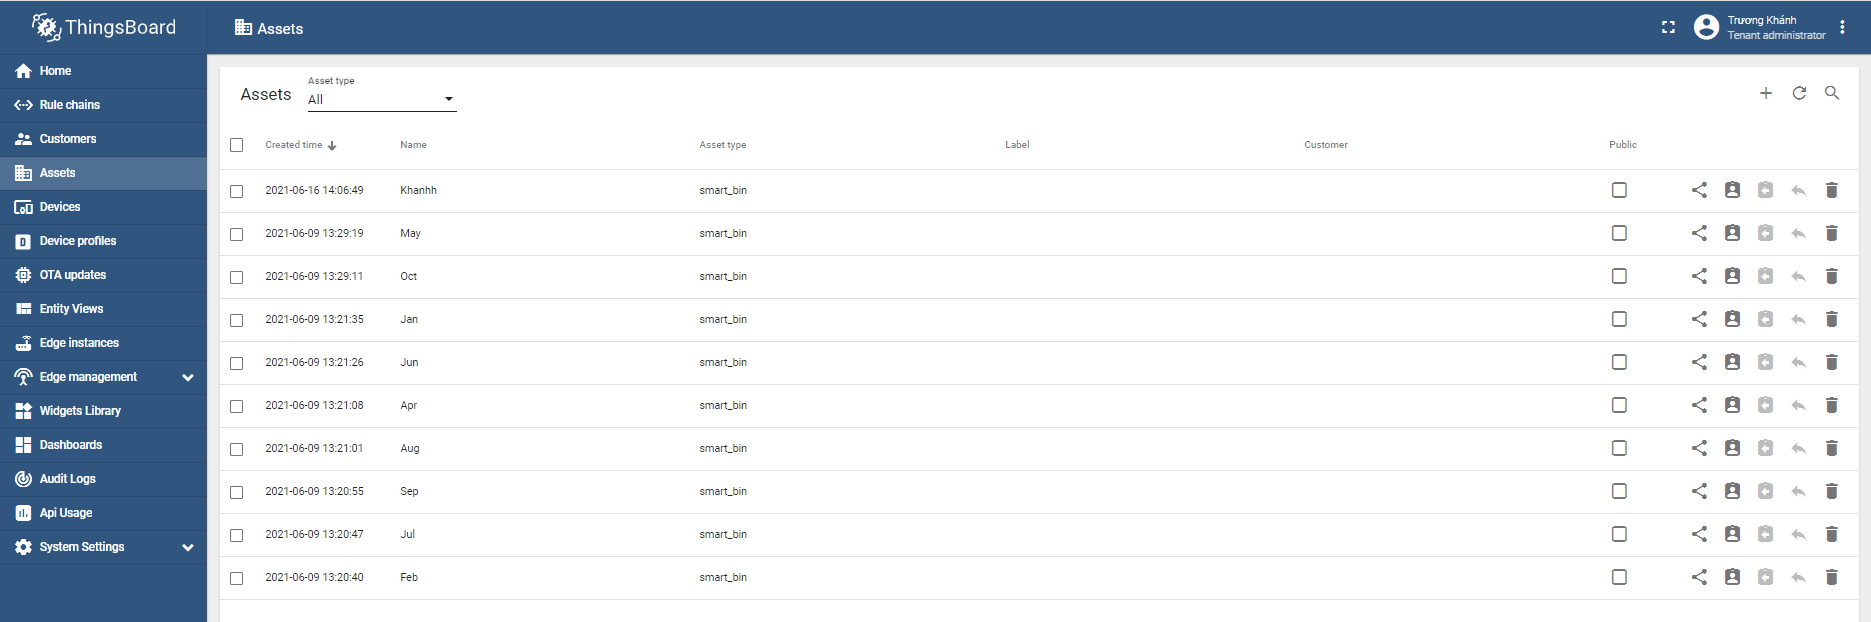
\includegraphics[width=\textwidth]{images/Khanh/Thingsboard/Assets.PNG}
    \caption{Danh sách thùng rác}
    \label{fig:asset_general}
\end{figure}
\begin{figure}[H]
    \centering
    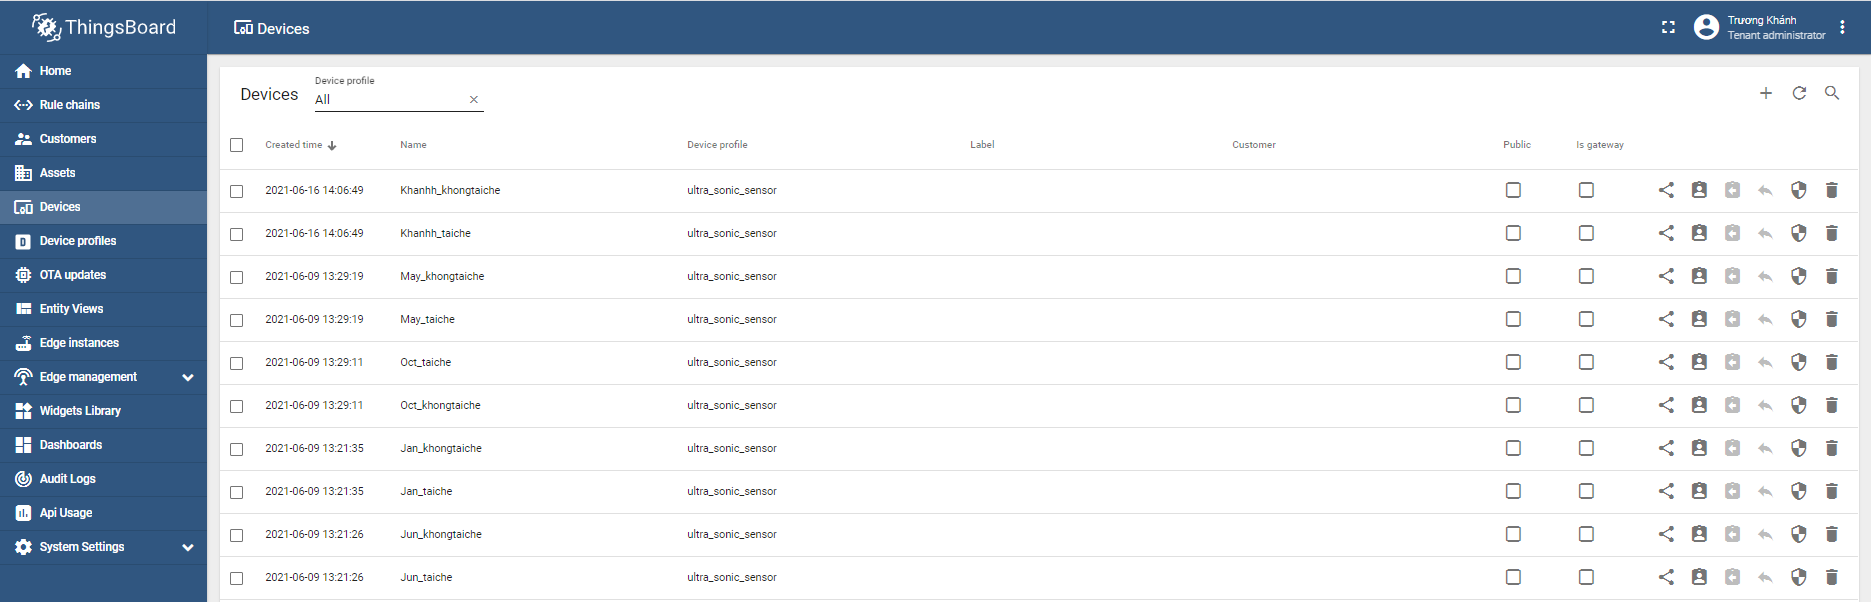
\includegraphics[width=\textwidth]{images/Khanh/Thingsboard/Devices.PNG}
    \caption{Danh sách cảm biến}
    \label{fig:device_general}
\end{figure}

Mỗi thực thể đều có những đặc điểm sau:
\begin{itemize}
    \item Details: chứa thông tin cơ bản của thực thể và một id phân biệt.
    \item Attributes: thuộc tính của thực thế, có thể cập nhật thủ công hoặc tự động thông qua Thingsboard API (hình \ref{fig:asset_attributes}).
    \item Lastest Telemetry: dữ liệu theo thời gian của thực thể, cập nhật thông qua Thingsboard API, mang giá trị gần đây nhất.
    \item Alarms: danh sách các báo động của thực thể.
    \item Events: các sự kiện giúp theo dõi tình trạng của thực thể.
    \item Relations: các mối quan hệ giữa các thực thể với nhau (hình \ref{fig:asset_relation}).
    \item Audit Logs: nhật ký kiểm tra theo dõi hành động người dùng liên quan đến các thực thể.
\end{itemize} 
\begin{figure}[H]
    \centering
    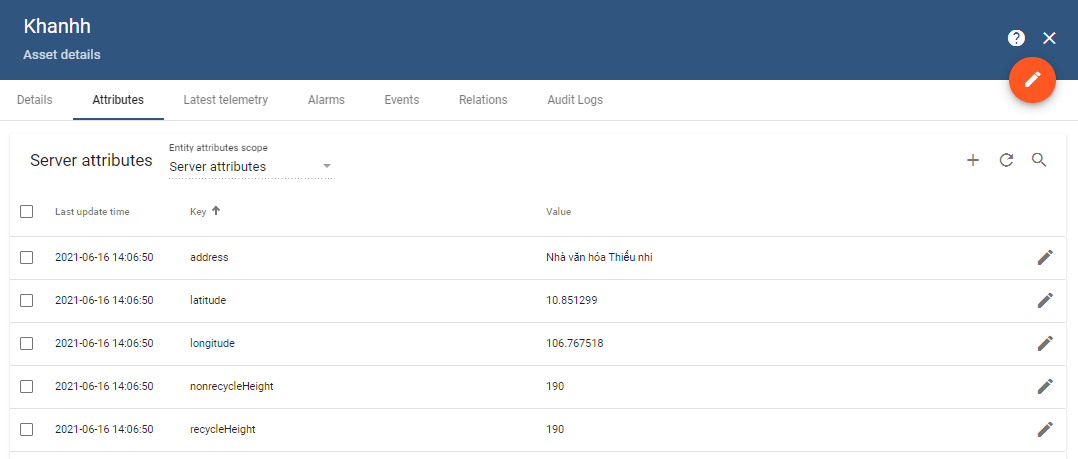
\includegraphics[width=\textwidth]{images/Khanh/Thingsboard/Asset_details.PNG}
    \caption{Thuộc tính thùng rác}
    \label{fig:asset_attributes}
\end{figure}
\begin{figure}[H]
    \centering
    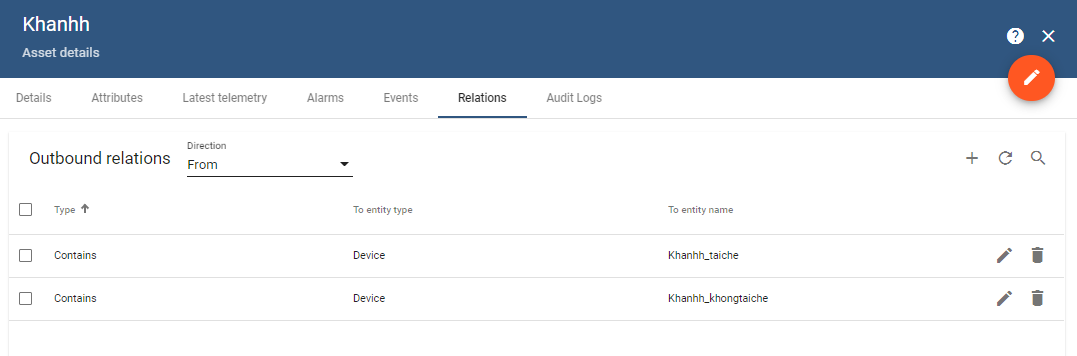
\includegraphics[width=\textwidth]{images/Khanh/Thingsboard/Asset_relation.PNG}
    \caption{Mối quan hệ của thùng rác với cảm biến}
    \label{fig:asset_relation}
\end{figure}

\subsection{Rule Chains}
Rule chains là những khung logic dạng kéo thả (nodes) được nối lại với nhau thành một chuỗi logic (rule chain) dùng để xử lý dữ liệu trực tiếp trên Thingsboard. Những nodes mà Thingsboard cung cấp đều có một chức năng khác nhau và được chia thành từng danh mục theo từng màu.
\begin{itemize}
    \item Filter (vàng): lọc những gói tin tới bằng những điều kiện được lập trình.
    \item Enrichment (xanh lá): thêm thông tin lấy từ thực thể và gắn vào gói tin. 
    \item Transformation (xanh dương): thay đổi thông tin gói tin bằng mã lập trình.
    \item Action (đỏ): tạo những action cho thực thể để xử lý dữ liệu.
    \item External (cam): tương tác với các hệ thống bên ngoài.
    \item Rule Chain (tím): gửi gói tin tới các rule chains khác.
\end{itemize}

Vì dữ liệu lượng rác được gửi từ các cảm biến và thùng rác phải sở hữu và định dạng lại dữ liệu để hiển thị lên biểu đồ đường, nên chúng tôi sử dụng rule chain để lưu dữ liệu vào cảm biến, đổi thực thể sở hữu sang thùng rác và định dạng lại dữ liệu thành chiều cao của thùng. Rule chain được mô tả ở hình \ref{fig:root_chain} và Delta chain \ref{fig:delta_chain}
\begin{figure}[H]
    \centering
    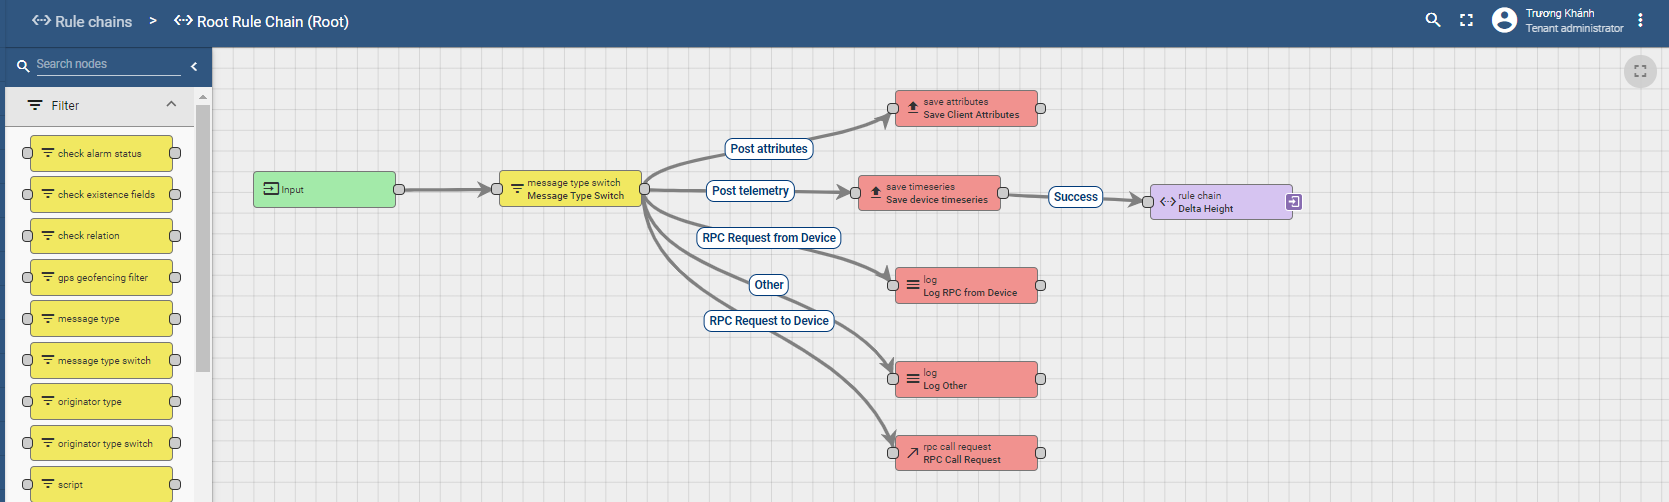
\includegraphics[width=\textwidth]{images/Khanh/Thingsboard/Root_rule_chain.PNG}
    \caption{Root Rule Chain}
    \label{fig:root_chain}
\end{figure}
Root Rule Chain là luồng xử lý chính cho Thingsboard, tất cả gói tin input được gửi từ hệ thống bên ngoài sẽ được lưu vào khung input. Sau đó gói tin sẽ được lọc theo \{MESSAGE\_TYPE\} bằng khung Message Type Switch, những \{MESSAGE\_TYPE\} bao gồm những sự kiện khác nhau liên quan đến thực thể. 

Những thuộc tính của thùng rác sẽ được lọc qua luồng Post attributes và được lưu vào thực thể, còn những dữ liệu thời gian của thùng rác và cảm biến sẽ được lọc qua luồng Post telemetry, được lưu vào thực thể và được gửi qua Delta Rule Chain. Những gói tin thuộc \{MESSAGE\_TYPE\} khác sẽ đi vào luồng khác hoặc được log qua Audit Logs.

\begin{figure}[H]
    \centering
    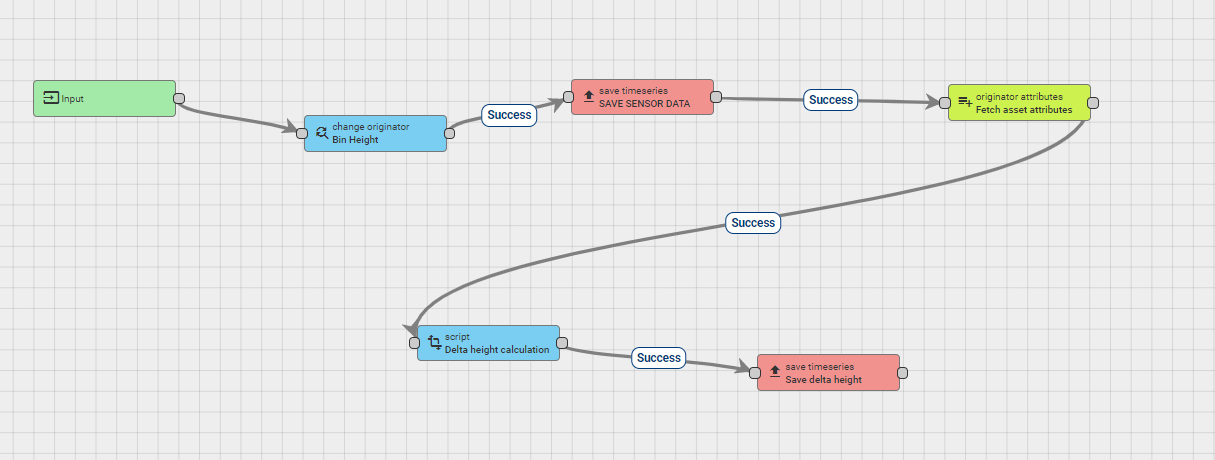
\includegraphics[width=\textwidth]{images/Khanh/Thingsboard/Delta_rule_chain.PNG}
    \caption{Delta-calculation Rule Chain}
    \label{fig:delta_chain}
\end{figure}

Gói tin được lọc từ type Post telemetry sẽ được lưu ở khung input, sau đó dữ liệu mức rác sẽ được chuyển thực thể từ cảm biến sang của thùng rác bằng khung Change originator và được lưu vào thùng rác.

Dữ liệu sau đó được định dạng lại giống chiều cao thùng rác bằng cách lấy chiều cao thùng trừ cho dữ liệu, vì thế sử dụng khung Originator attributes để fetch thuộc tính thực thể và đưa tất cả qua một Transformation script để xử lý logic.

Xử lý dữ liệu mức rác cũng khá đơn giản khi chỉ cần phân chia dữ liệu tái chế và không tái chế và lấy ngăn chiều cao trừ cho dữ liệu, kết quả gửi qua khung Save timeseries để lưu dữ liệu vào thùng rác.

\subsection{Dashboard}
Dashboard là khung màn hình hiển thị chính của Thingsboard, được tạo bởi các widget hỗ trợ sẵn (biểu đồ, bản đồ, bảng, input tương tác, alarms, ...), hỗ trợ hiển thị, tương tác và trực quan hóa dữ liệu theo nhiều cách. 

Dashboard cho phép chúng ta tạo ra nhiều các dashboard khác, trong một dashboard, ta có thể có nhiều state và action event để di chuyển giữa các state, nhiều Entity aliases để phân biệt và gom cụm các thực thể lại với nhau và thêm vào các widget để lấy dữ liệu dễ dàng hơn.

Ở trang dashboard chính, chúng tôi cho hiển thị bản đồ hiện tất cả những thùng rác được tạo như hình \ref{fig:dashboard_map} và một danh sách các thùng rác gồm các thuộc tính của nó như hình \ref{fig:dashboard_asset_list}

\begin{figure}[H]
    \centering
    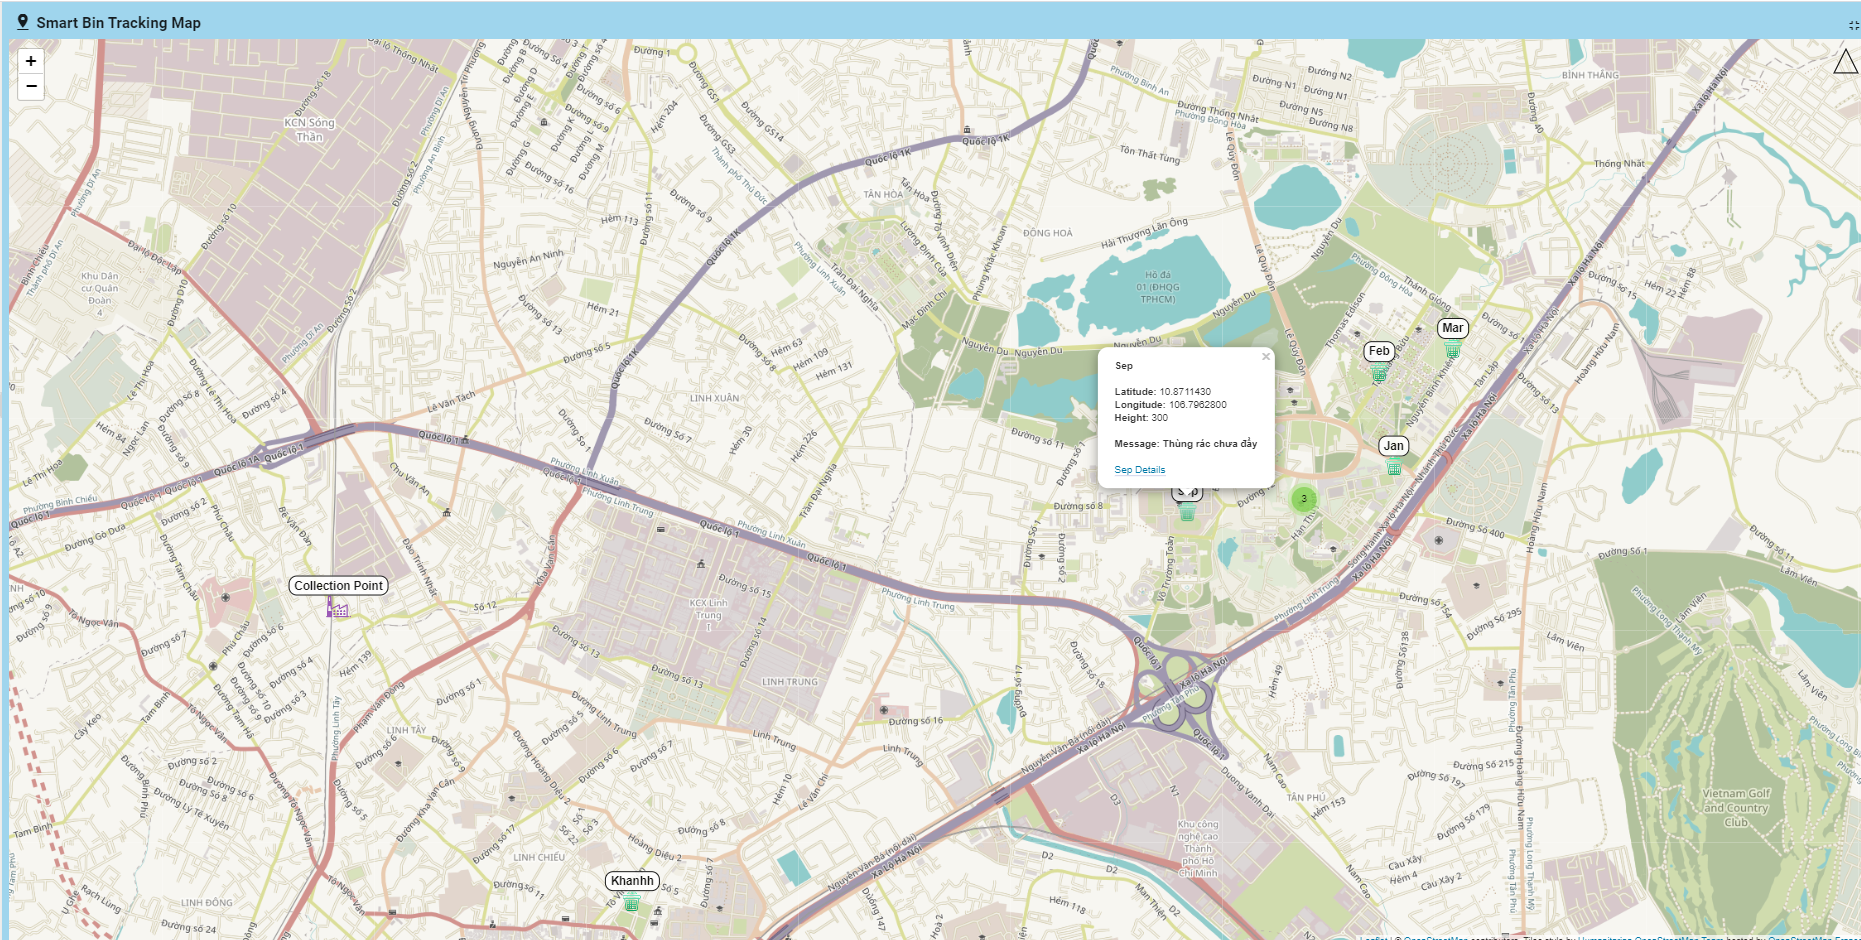
\includegraphics[width=\textwidth]{images/Khanh/Thingsboard/Dashboard_map.PNG}
    \caption{Bản đồ theo dõi vị trí thùng rác}
    \label{fig:dashboard_map}
\end{figure}
Bản đồ hiển thị tất cả các thùng rác và địa điểm thu gom rác, được phân biệt bằng icon khác nhau và các thùng rác được clustering để gom cụm từng vùng. Với mỗi thùng rác, khi nhận được trạng thái đầy sẽ chuyển thành màu đỏ để dễ nhận biết. Ngoài ra, mỗi thùng rác còn có tooltip hiện tên, tọa độ, chiều cao, chuỗi thông báo và một đường link dẫn đến state chi tiết của thùng rác. 

Bản đồ này cũng tích hợp tính năng Polygon để vẽ tuyến đường, có thể thích ứng với chức năng tìm đường tối ưu nhất từ nơi gom rác đến tất cả thùng rác đầy như hình \ref{fig:map_optimization}.
\begin{figure}[H]
    \centering
    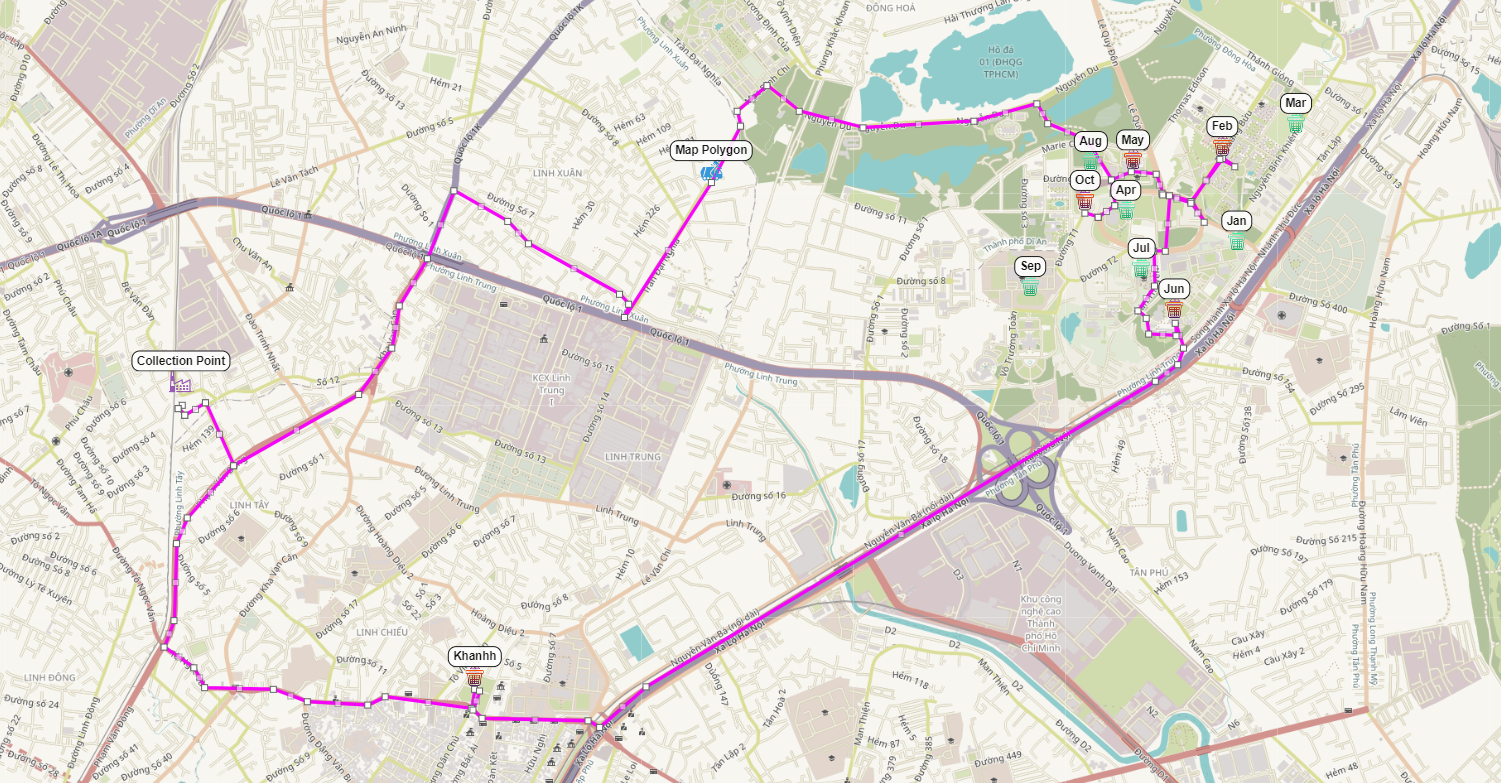
\includegraphics[width=\textwidth]{images/Khanh/Thingsboard/Road_optimization.PNG}
    \caption{Polygon các tọa độ đường đi trên bản đồ}
    \label{fig:map_optimization}
\end{figure}

\begin{figure}[H]
    \centering
    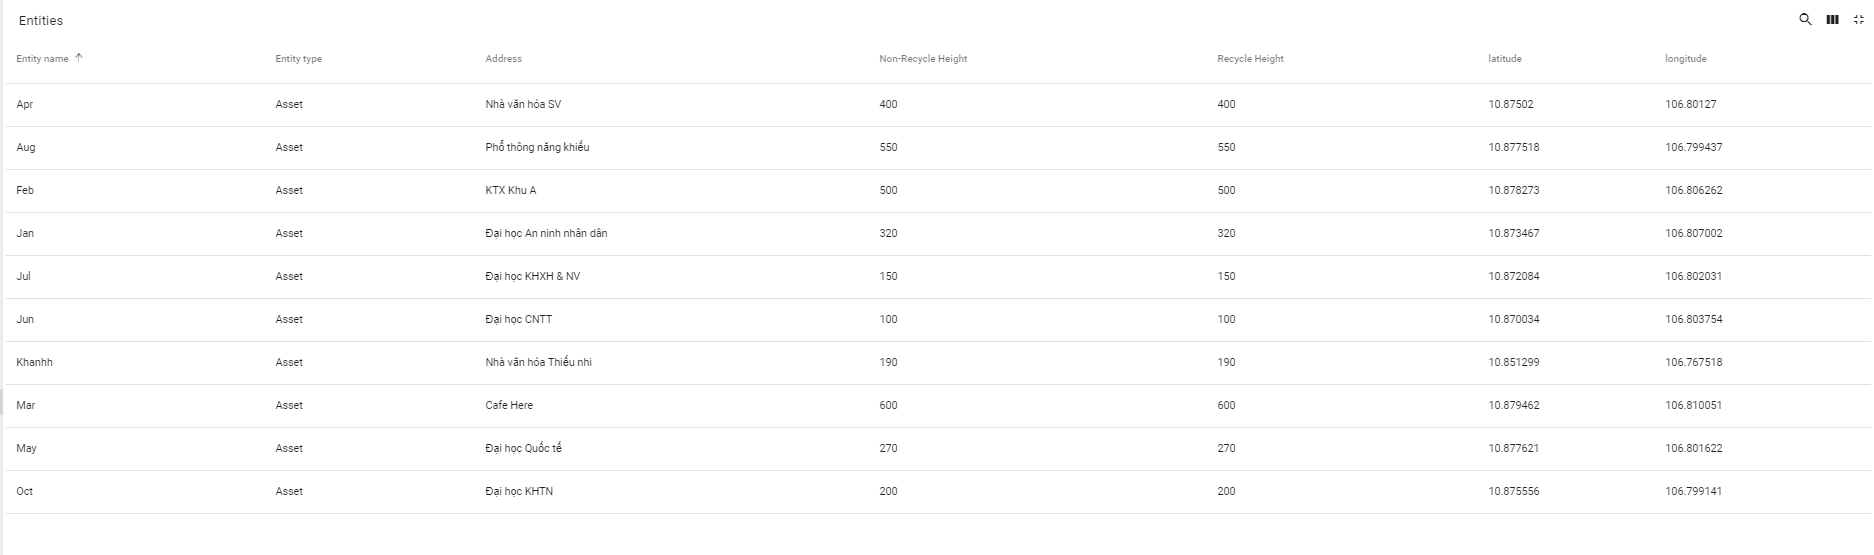
\includegraphics[width=\textwidth]{images/Khanh/Thingsboard/Dashboard_list.PNG}
    \caption{Danh sách thùng rác hiện có}
    \label{fig:dashboard_asset_list}
\end{figure}
Danh sách các thùng rác bao gồm tên, loại, địa chỉ, tọa độ và chiều cao hai ngăn của thùng, mỗi thùng rác được gắn sự kiện event khi nhấn vào thì sẽ chuyển qua state dashboard khác, cụ thể là state hiển thị dữ liệu của thùng rác và các cảm biến của nó.

Ở state dashboard chi tiết từng thùng rác, giao diện được bố trí như hình \ref{fig:bin_detail}, với một biểu đồ đường hiển thị mức rác tái chế và không tái chế của thùng, ở dưới bên trái là danh sách các cảm biến của thùng rác cùng với dữ liệu của cảm biến, còn ở bên phải là bảng thông báo tình trạng của thùng rác bao gồm tình trạng chưa đầy, đã đầy hoặc dự tính đã đầy trong một khoảng thời gian tới. 
\begin{figure}[H]
    \centering
    \includegraphics[width=\textwidth]{images/Khanh/Thingsboard/Bin_detail.PNG}
    \caption{Giao diện chi tiết của thùng rác thông minh}
    \label{fig:bin_detail}
\end{figure}

Khi nhấn vào mỗi cảm biến của thùng rác, dashboard sẽ chuyển sang state mới hiển thị biểu đồ dữ liệu của cảm biến theo thời gian như hình \ref{fig:sensor_detail}.
\begin{figure}[H]
    \centering
    \includegraphics[width=\textwidth]{images/Khanh/Thingsboard/Sensor_detail.PNG}
    \caption{Biểu đồ thể hiện dữ liệu của cảm biến}
    \label{fig:sensor_detail}
\end{figure}
% !TEX root = ..\thesis.tex


\chapter{Khó khăn, so sánh và hướng phát triển}


\section{Khó khăn}
Khi setup node, nhóm gặp vấn đề về frequency, node không thể gửi data cho gateway


% % !TEX root = ..\thesis.tex
% \nheading{TÀI LIỆU THAM KHẢO}


% \printbibliography

\begin{thebibliography}{SJL05}

\bibitem{trashnet} Gary Thung, Mindy Yang. \textit{Classification of trash for recyclability status}.CS229 Project Report2016, 2016.

\bibitem{smartcity} De Carolis, Berardina, Francesco Ladogana, and Nicola Macchiarulo.\textit{YOLO TrashNet: Garbage Detection in Video Streams.} 2020 IEEE Conference on Evolving and Adaptive Intelligent Systems (EAIS). IEEE, 2020.
%\bibitem{DBPedia} Bizer, Christian, Jens Lehmann, Georgi Kobilarov, Sören Auer, Christian Becker, Richard Cyganiak, and Sebastian Hellmann. "DBpedia-A crystallization point for the Web of Data." Web Semantics: science, services and agents on the world wide web 7, no. 3 (2009): 154-165.
\bibitem{lstmevaluation} Ralf C. Staudemeyer, Christian W. Omlin. \textit{Evaluating performance of long short-term memoryrecurrent neural networks on intrusion detection data}. Proceedings of the South African Institute for Computer Scientists and Information Technologists Conference 2013

\bibitem{lstmprediction} Athar Khodabakhsh, Ismail Ari, Mustafa Bakir, Serhat Murat Alagoz. \textit{Forecasting Multivariate Time-Series Data using LSTM and Mini-batches}. Data Science: From Research to Application 2020

\bibitem{lstmmultivariateprediction} Jason Brownlee. \textit{Multivariate Time Series Forecasting with LSTMs in Keras} in Deep Learning for Time Series 2017.

\bibitem{nodejsserver} S. L. Bangare, S. Gupta, M. Dalal, A. Inamdar. \textit{Using Node.Js to Build High Speed and Scalable Backend Database Server}. International Journal of Research in Advent Technology (E-ISSN: 2321-9637) Special Issue National Conference “NCPCI-2016”, 2016 

\bibitem{mapbox} Mapbox API 2021 Mapbox Inc. [Online]. Available: https://docs.mapbox.com/api/

\bibitem{thingsboard} Thingsboard API 2021 created by Thingsboard team. [Online]. Available: http://demo.thingsboard.io/swagger-ui.html

\end{thebibliography}

\end{document}
